%
% main.tex -- Paper zum Thema <reedsolomon>
%
% (c) 2020 Hochschule Rapperswil
%
\chapter{Reed-Solomon-Code\label{chapter:reedsolomon}}
\lhead{Thema}
\begin{refsection}
\chapterauthor{Joshua Bär und Michael Steiner}

Ein paar Hinweise für die korrekte Formatierung des Textes
\begin{itemize}
\item
Absätze werden gebildet, indem man eine Leerzeile einfügt.
Die Verwendung von \verb+\\+ ist nur in Tabellen und Arrays gestattet.
\item
Die explizite Platzierung von Bildern ist nicht erlaubt, entsprechende
Optionen werden gelöscht. 
Verwenden Sie Labels und Verweise, um auf Bilder hinzuweisen.
\item
Beginnen Sie jeden Satz auf einer neuen Zeile. 
Damit ermöglichen Sie dem Versionsverwaltungssysteme, Änderungen
in verschiedenen Sätzen von verschiedenen Autoren ohne Konflikt 
anzuwenden.
\item 
Bilden Sie auch für Formeln kurze Zeilen, einerseits der besseren
Übersicht wegen, aber auch um GIT die Arbeit zu erleichtern.
\end{itemize}

% Joshua
%
% einleitung.tex -- Beispiel-File für die Einleitung
%
% (c) 2020 Prof Dr Andreas Müller, Hochschule Rapperswil
%
\section{Teil 0\label{clifford:section:teil0}}
\rhead{Teil 0}
Lorem ipsum dolor sit amet, consetetur sadipscing elitr, sed diam
nonumy eirmod tempor invidunt ut labore et dolore magna aliquyam
erat, sed diam voluptua \cite{clifford:bibtex}.
At vero eos et accusam et justo duo dolores et ea rebum.
Stet clita kasd gubergren, no sea takimata sanctus est Lorem ipsum
dolor sit amet.

Lorem ipsum dolor sit amet, consetetur sadipscing elitr, sed diam
nonumy eirmod tempor invidunt ut labore et dolore magna aliquyam
erat, sed diam voluptua.
At vero eos et accusam et justo duo dolores et ea rebum.  Stet clita
kasd gubergren, no sea takimata sanctus est Lorem ipsum dolor sit
amet.



%
% teil1.tex -- Beispiel-File für das Paper
%
% (c) 2020 Prof Dr Andreas Müller, Hochschule Rapperswil
%
%
% teil2.tex -- Beispiel-File für teil2 
%
% (c) 2020 Prof Dr Andreas Müller, Hochschule Rapperswil
%%



\rhead{Kalman-Filter}

\section{Kalman-Filter}
Da wir die äussere Kraft nicht direkt messen können, benötigen wir ein Werkzeug, welches aus der gemessenen Position, die Krafteinwirkung auf unsere System schätzt. 
Dies ist eine Typische Anwendung für den linearen Kalman-Filter.
Unser Ziel ist es, anhand der Messung die eigentlich interessante Grösse $f$ zu bestimmen. 
Dabei wird durch eine deterministische Vorhersage, in dem der Zustand * Eigendynamik des Systems gerechnet. 
Die Idee dahinter ist, dass das Kalman-Filter die nicht-deterministische Grösse $f$ anhand der Messung und der Vorhersage zu bestimmen.

Für mehrere Dimensionen (x,y,z) würde der Pythagoras für das System benötigt werden.
Da sich der Pythagoras bekanntlich nicht linear verhält, kann kein lineares Kalman-Filter implementiert werden. 
Da das Kalman-Filter besonders effektiv und einfach für lineare Abläufe geeignet ist, würde eine zweidimensionale Betrachtung den Rahmen dieser Arbeit sprengen. 
Für ein nicht-lineares System werden Extended Kalman-Filter benötigt, bei denen die System-Matrix (A) durch die Jacobi-Matrix des System ersetzt wird.
Einfachheitshalber beschränken wir uns auf den linearen Fall, da dadurch die wesentlichen Punkte bereits aufgezeigt werden. 

\subsection{Geschichte}
Das Kalman-Filter wurde 1960 von Rudolf Emil Kalman entdeckt und direkt von der NASA für die Appollo Mission benutzt. Der Filter kommt mit wenig Rechenleistung aus und war somit dafür geeignet die Rakete bei der Navigation zu unterstützen. Das Filter schätzt den Zustand eines Systems anhand von Messungen und kann den nächsten Zustand errechnen. Eine typische Anwendungen des Kalman-Filters ist Glättung von verrauschten Daten und die Schätzung von Parametern. Dies kommt heutzutage in jedem Satellit, Navigationssystem, Smartphones und Videospielen vor.

\subsection{Wahrscheinlichkeit}
Das Kalman-Filter schätzt den wahrscheinlichsten Wert zwischen Normalverteilungen.
Dies bedeutet, das Filter schätzt nicht nur den Mittelwert, sondern auch die Standartabweichung.
Da Normalverteilungen dadurch vollständig definiert sind, schätzt ein Kalman-Filter die gesamte Verteilungsfunktion des Zustandes.
Die eine Funktion zeigt die errechnete Vorhersage des Zustands, bzw. deren Normalverteilung. 
Die andere Funktion zeigt die verrauschte Messung des nächsten Zustand, bzw. deren Normalverteilung. 
Wie man am Beispiel der Gauss-Verteilungen unten sehen kann, ist sowohl der geschätzte Zustand als auch der gemessene Zustand normalverteilt und haben dementsprechend unterschiedliche Standardabweichungen $\sigma$ und Erwartungswerte $\mu$.

\begin{figure}
 \begin{center}
 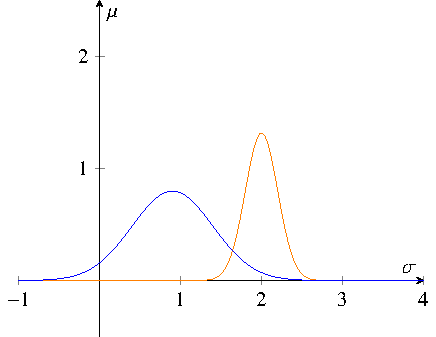
\includegraphics[width=5cm]{papers/erdbeben/Gausskurve2.pdf}
 \caption{Zwei Normalerteilungen; Die eine Funktion zeigt die Vorhersage, die andere die Messung}
 \end{center}
\end{figure}


Um eine genauere Schätzung des Zustandes zu machen, wird nun ein Wert zwischen den beiden Verteilungen berechnet. 
Nun wird eine Eigenschaft der Normalverteilung ausgenutzt. Durch das Multiplizieren zweier Normalverteilungen entsteht eine neue Normalverteilung. 
Wir haben eine Normalverteilung der Vorhersage:

\[ {y_1}(x;{\mu_1},{\sigma_1})=\frac{1}{\sqrt{2\pi\sigma_1^2}}\quad e^{-\frac{(x-{\mu_1})^2}{2{\sigma_1}^2}} \]
und der Messung:
\[ {y_2}(x;{\mu_2},{\sigma_2})=\frac{1}{\sqrt{2\pi\sigma_2^2}}\quad e^{-\frac{(x-{\mu_2})^2}{2{\sigma_2}^2}}. \]



Diesen werden nun Multipliziert und durch deren Fläche geteilt um sie wieder zu Normieren:
\[
{y_f}(x;{\mu_f},{\sigma_f})=\frac{ \frac{1}{\sqrt{2\pi\sigma_1^2}}e^{-\frac{(x-{\mu_1})^2}{2{\sigma_1}^2}} \cdot \frac{1}{\sqrt{2\pi\sigma_2^2}}e^{-\frac{(x-{\mu_2})^2}{2{\sigma_2}^2}}}{\int {y_1}\cdot{y_2} dx\,}
 \] 

Diese Kombination der beiden Verteilungen resultiert wiederum in einer Normalverteilung
\[ {y_f}(x; {\mu_f}, {\sigma_f}) = {y_1}(x;{ \mu_1},{ \sigma_1}) {\cdot y_2}(x; {\mu_2}, {\sigma_2}), \]
mit Erwartungswert
\[ \mu_f = \frac{\mu_1\sigma_2^2 + \mu_2 \sigma_1^2}{\sigma_1^2 + \sigma_2^2} \]
und Varianz
\[ \sigma_f^2 = \frac{\sigma_1^2 \sigma_2^2}{\sigma_1^2 + \sigma_2^2}. \]

Dadurch gleicht sich die neue Kurve den anderen an. Interessant daran ist, dass die fusionierte Kurve sich der genauere Normal-Verteilung anpasst.
Ist ${\sigma_2}$ klein und ${\sigma_1}$ gross, so wird sich die fusionierte Kurve näher an ${y_2}(x;{\mu_2},{\sigma_2})$ begeben.
Sie ist also gewichtet und die best mögliche Schätzung. 


\begin{figure}
 \begin{center}
 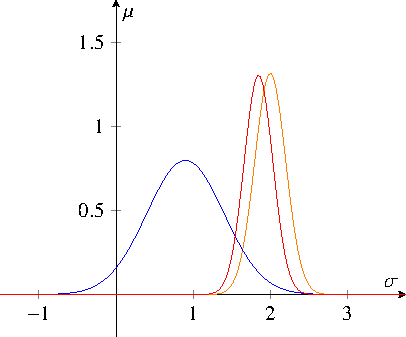
\includegraphics[width=5cm]{papers/erdbeben/Gausskurve3.pdf}
 \caption{Durch das Multiplizieren der blauen und der orangen Verteilung entsteht die die rote, optimale Funktion}
 \end{center}
\end{figure}


Was in 2 Dimensionen erklärt wurde, funktioniert auch in mehreren Dimensionen. 
Dieses Prinzip mach sich das Kalman Filter zu nutze, und wird von uns für die Erdbeben Berechnung genutzt. 

\section{Filter-Matrizen}
Um den Kalman Filter zu starten, müssen gewisse Bedingungen definiert werden. 
In diesem Abschnitt werden die einzelnen Parameter und Matrizen erklärt und erläutert, wofür sie nützlich sind. 

\subsection{Anfangsbedingungen}
\subsubsection*{Anfangszustand $x$}
Das Filter benötigt eine Anfangsbedingung. 
In unserem Fall ist es die Ruhelage, die Masse bewegt sich nicht. 
Zudem erfährt die Apparatur keine äussere Kraft.


\[ {x_0 }= \left( \begin{array}{c} {s_0}\\ {v_0}\\{f_0}\end{array}\right) = \left( \begin{array}{c} 0\\ 0\\ 0\end{array}\right) \]

\subsubsection*{Anfangsfehler / Kovarianzmatrix $P$}
Da auch der Anfangszustand fehlerhaft sein kann, wird für das Filter ein Anfangsfehler verwendet. 
Auf der Diagonalen werden die Varianzen eingesetzt, in den restlichen Felder stehen die Kovarianzen.
Zur Erinnerung: Die Varianz ist ein Mass für die Streuung eines Wertes, die Kovarianz hingegen beschreibt die Abhängigkeit der Streuungen zweier Werte.

Kovarianz: Cov(x, y) und Varianz: Var(x) = Cov(x, x)

In unserem Fall ist der Anfangszustand gut bekannt. 
Wir gehen davon aus, dass das System in Ruhe und in Abwesenheit eines Erdbeben startet, somit kann die Matrix mit Nullen bestückt werden. 
Als Initialwert für die für die Kovarianzmatrix ergibt sich

\[ 
{P_0 }=
\left(
\begin{array}{ccc} 	
0 & 0 &0 \\ 
0 &0 & 0 \\ 
0 & 0 &0 \\
\end{array}
\right).
 \] 
Diese Matrix beschreibt die Unsicherheit des geschätzten Zustandes und wird sowohl für die Vorhersage als auch die Korrektur benötigt. 
Sie wird nach jeder Schätzung aktualisiert. 
Für einen gut bekannten Zustandsvektor können kleine Werte eingesetzt werden, für ungenaue Anfangsbedingungen sollten grosse Werte verwendet werden. 
Grosse Werte ermöglichen dem Filter sich schnell einzupendeln. 

\subsubsection*{Dynamikmatrix $A$}
Das Kalman-Filter benötigt für die Vorhersage des nächsten Zustandes eine Beschreibung der Systemdynamik.
Die Dynamikmatrix bildet den Kern des Filters. Diese wurde weiter oben bereits beschrieben. 
Dabei wollen wird die äussere Kraft des Systems ermitteln.
Da nichts über die äussere Kraft bekannt ist, müssen wir annehmen das deren Ableitung 0 ist. 
Die System Vektor-Gleichung lautet daher:
\[ 
A = \left(
 \begin{array}{ccc} 	
0 & 1& 0 \\
- \frac{D}{m} &-\frac{2k}{m} & \frac{1} {m}\\
0 & 0& 0\\ 
\end{array}\right)  
 \]
Dabei soll der Kalman-Filter in diskreten Zeitschritten $\Delta t$ arbeiten. 
Die Übergangs-Matrix erhalten wir aus der Systemdynamikmatrix mittels Exponentialfunktion: 
\[\Phi = \exp(A\Delta t). \]

\subsubsection*{Prozessrauschkovarianzmatrix $Q$}
Die Prozessrauschmatrix teilt dem Filter mit, wie sich der Prozess verändert. 
Kalman-Filter berücksichtigen Unsicherheiten wie Messfehler und -rauschen. 
Bei unserem Modell könnte das beispielsweise ein Windstoss an die Masse sein. 
Für uns wäre dies:
\[ 
Q = \left(
 \begin{array}{ccc} 	
{\sigma_s }^2& 0& 0 \\ 
0 & {\sigma_v }^2& 0\\ 
0 & 0& {\sigma_f }^2\\
\end{array}\right)  
 \]

Die Standabweichungen müssten statistisch ermittelt werden, da der Fehler nicht vom Sensor kommt und somit nicht vom Hersteller gegeben ist. 
Das Bedeutet wiederum dass $Q$ die Unsicherheit des Prozesses beschreibt und nicht die der Messung.

\subsubsection*{Messmatrix $H$}
Die Messmatrix gibt an, welche Parameter gemessen werden
In unserem Falle ist es die Position der Massen. 

\[ H = (1, 0, 0) \]

\subsubsection*{Messrauschkovarianz $R$}
Die Messrauschkovarianzmatrix beinhaltet, wie der Name es schon sagt, das Rauschen der Positionsmessung. 
In unserem Fall wird nur die Position der Masse gemessen. Da wir keine anderen Sensoren haben ist $R$ lediglich:
\[ R= ({\sigma_{sensor}}^2).
 \] 
Diese Messrauchen wird meistens vom Sensorhersteller angegeben. 
Für unsere Theoretische Apparatur wird hier ein kleiner Fehler eingesetzt da heutige Sensoren sehr genau messen können. 

\subsection{Fiter-Agorithmus}
Nachdem alle Parameter aufgestellt sind, wird das Filter initialisiert.
Zuerst wird der nächste Zustand der Feder vorhergesagt, danach wird die Messung präzisiert und laufend zu aktualisieren. 
Das Filter berechnet aufgrund der aktuellen Schätzung eine Vorhersage. 
Diese wird, sobald verfügbar, mit der Messung verglichen. 
Aus dieser Differenz und den Unsicherheiten des Prozesses ($Q$) und der Messung ($R$) wird der wahrscheinlichste, neue Zustand geschätzt.

\subsubsection*{Vorhersage}
Im Filterschritt Vorhersage wird der nächste Zustand anhand des Anfangszustand und der Systemmatrix berechnet. 
Dies funktioniert mit dem Rechenschritt:
\[ 
{x_{k|k-1}}=\Phi \cdot {x_{k-1|k-1}}= \exp(A\Delta t)\cdot{x_{k|k-1}}.
 \] 

Die Kovarianz $P_{pred}$ wird ebenfalls neu berechnet. Da wir ein mehrdimensionales System haben, kommt noch die Prozessunsicherheit $Q$ dazu, so dass die Unsicherheit des Anfangsfehlers $P$ laufend verändert. 
Dies funktioniert durch multiplizieren der Systemmatrix mit dem aktualisierten Anfangsfehler. 
Dazu wird noch die Prozessunsicherheit addiert, somit entsteht die Gleichung
\[ {P_{k|k-1}} = {\Phi_k}  {P_{k-1|k-1}} {\Phi_k} ^T + {Q_{k-1}} .\] 
Es vergeht genau $dt$ Zeit, und dieser Vorgang wird wiederholt. 
Dabei wird in den späteren Schritten überprüft, wie genau die letzte Anpassung von $P$ zur Messung stimmt. 
Ist der Unterschied klein, wird die Kovarianz $P$ kleiner, ist der Unterschied gross, wird auch die Kovarianz grösser. 
Das Filter passt sich selber an und korrigiert sich bei grosser Abweichung.

\subsubsection*{Messen}
Der Sensor wurde noch nicht benutz, doch genau der liefert Werte für das Filter. 
Die aktuellen Messwerte $z$ werden die Innovation $w$ mit dem Zustandsvektor $x$ und der Messmatrix $H$ zusammengerechnet.
Hier bei wird lediglich die Messung mit dem Fehler behaftet, und die Messmatrix $H$ mit der Vorhersage multipliziert

\[{w_{k}}={z_{k}}-{H_{k}}\cdot{x_{k|k-1}}.\] 

Die Innovation ist der Teil der Messung, die nicht durch die Systemdynamik erklärt werden kann. 
Die Hilfsgröße Innovation beschreibt, wie genau die Vorhersage den aktuellen Messwert mittels der Systemmatrix $\phi$ beschreiben kann. 
Für eine schlechte Vorhersage wird die dazugehörige Innovation gross, für eine genaue Vorhersage dagegen klein sein. 
Entsprechende Korrekturen müssen dann gross bzw. nur gering ausfallen. 
Innovation = Messung - Vorhersage. Dies ist intuitiv logisch, eine Innovation von 0 bedeutet, dass die Messung nichts Neues hervorbrachte.

Im nächsten Schritt wir analysiert, mit welcher Kovarianz weiter gerechnet wird. 
Hierbei wird die Unsicherheit $P$, die Messmatrix $H$ und die Messunsicherheit $R$ miteinander verrechnet. 
\[ 
{S_{k}}={H_{k}}{P_{k|k-1}}{H_{k}}^T+{R_{k}}
 \] 

\subsubsection*{Aktualisieren}
Im nächsten Schritt kommt nun die Wahrscheinlichkeit nach Gauss dazu. 
\[ 
{K_{k}}= {{P_{k|k-1}} \cdot {H_{k}^T}}\cdot {S_{k}}^{-1} 
 \] 
Dieser Vorgang wird Kalman-Gain genannt. 
Er sagt aus, welcher Kurve mehr Vertraut werden soll, dem Messwert oder der Systemdynamik.
Das Kalman-Gain wird geringer wen der Messwert dem vorhergesagten Systemzustand entspricht. 
Sind die Messwerte komplett anders als die Vorhersage, wo werden die Elemente in der Matrix $K$ grösser.
Anhand der Informationen aus dem Kalman-Gain $K$ wird das System geupdated.

\[ 
{x_{k|k}}={x_{k|k-1}}+({K_{k}}\cdot {w_{k}}) 
 \] 

Dazu kommt  eine neue Kovarianz für den nächste Vorhersageschritt:

\[ 
{P_{k|k}}=(I-({K_{k}} \cdot {H_{k}})) \cdot {P_{k|k-1}}  
 \] 

Der ganze Ablauf wird nun zum Algorithmus und beginnt wieder mit der Vorhersage 

\[ 
{x_{k|k-1}}=\Phi \cdot {x_{k-1|k-1}}= \exp(A\Delta t)\cdot{x_{k|k-1}}.
 \] 


\subsection{Zusammenfassung }
Zusammenfassend kann das Kalman-Filter in offizieller Typus dargestellt werden. 
Dabei beginnt das Filter mit dem Anfangszustand für $k=0$

1. Nächster Zustand vorhersagen
\[{x_{k|k-1}}=\Phi \cdot {x_{k-1|k-1}}= \exp(A\Delta t)\cdot{x_{k|k-1}}.\] 

2. Nächste Fehlerkovarianz vorhersagen
\[{P_{k|k-1}}={\Phi _{k}} {P_{k-1|k-1}} {\Phi _{k}}^T + {Q_{k-1}}.\] 

3. Das Kalman Filter anwenden
\[{K_{k}}= {P_{k|k-1}} \cdot {H_{k}^T}\cdot {S_{k}^{-1}}\] 

4. Schätzung aktualisieren
\[{x_{k|k}}={x_{k|k-1}}+({K_{k}}\cdot {w_{k}}) \] 

5. Fehlerkovarianz aktualisieren
\[{P_{k|k}}=(I-({K_{k}}\cdot {H_{k}})) \cdot {P_{k|k-1}} \] 


6. Die Outputs von $k$ werden die Inputs für ${k-1}$ und werden wieder im Schritt 1 verwendet


%
% teil2.tex -- Beispiel-File für teil2 
%
% (c) 2020 Prof Dr Andreas Müller, Hochschule Rapperswil
%
\section{Fraktale mit IFS 
\label{ifs:section:teil2}}
\rhead{Teil 2}
Wollen wir nun eine bestimmte Art anschauen, wie man Fraktale machen kann.
Zur Veranschaulichung dieser Methode nehmen wir das Sierpinski Dreieck.
\begin{figure}
	\centering
	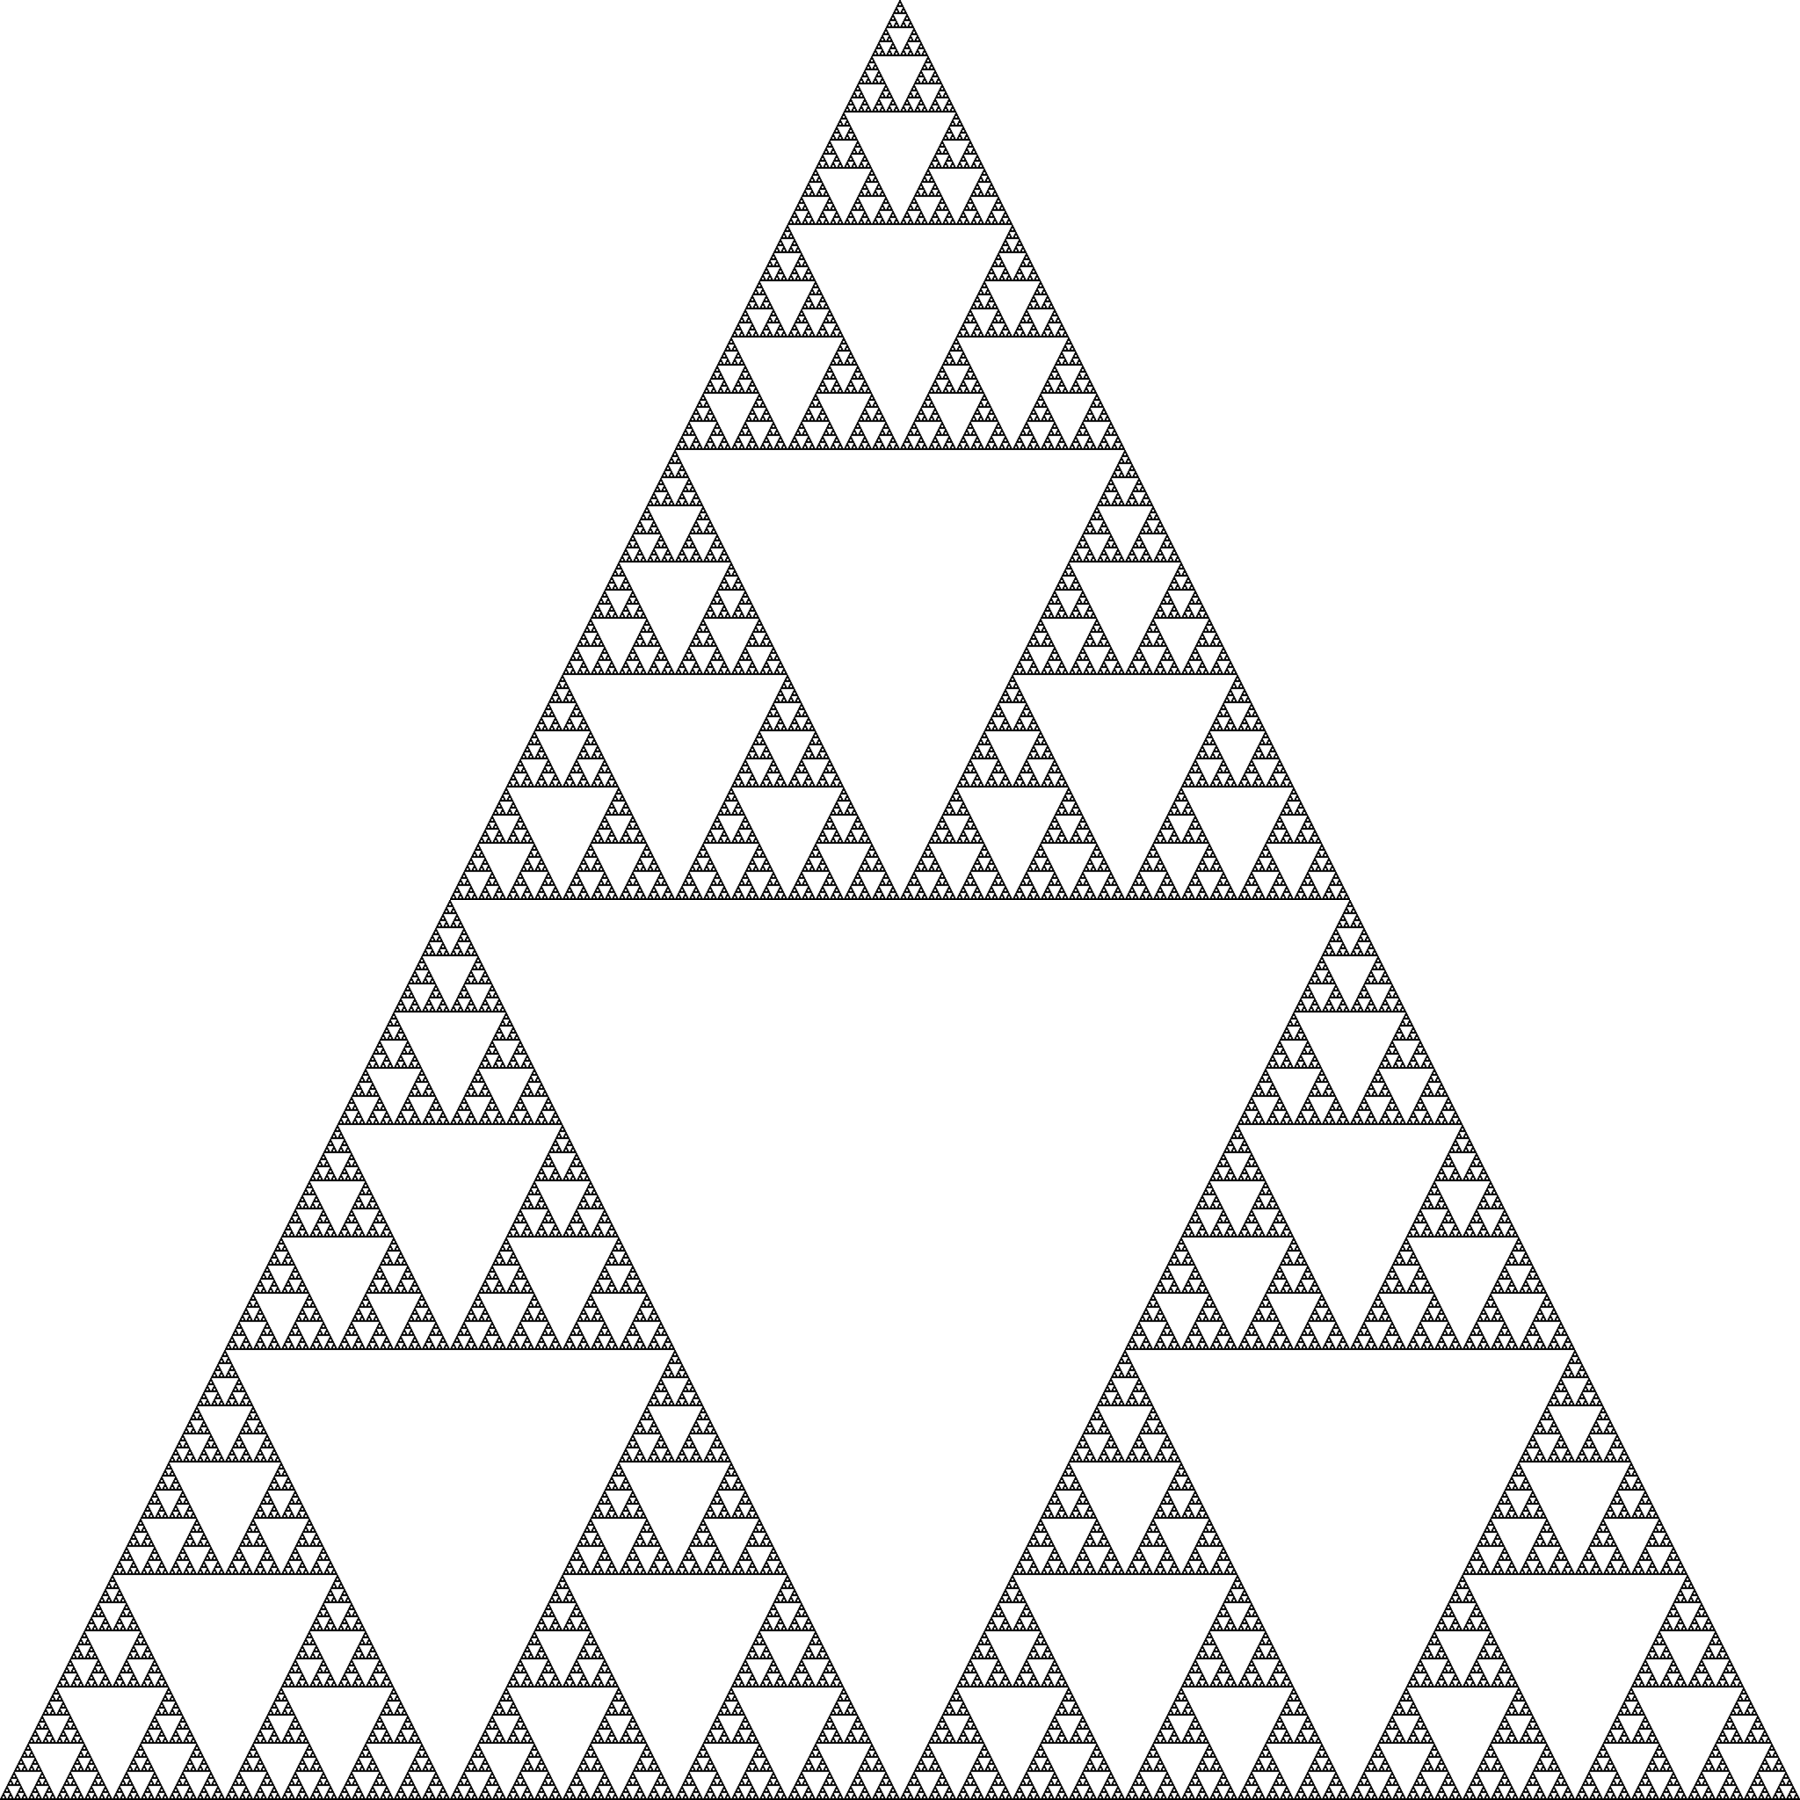
\includegraphics[width=0.5\textwidth]{papers/ifs/images/sierpinski}
	\caption{Sierpinski-Dreieck}
	\label{ifs:sierpinski10}
\end{figure}
Es besteht aus drei kleineren Kopien von sich selbst.
Es ist also ein Selbstähnliches Gebilde.
Diese Eigenschaft wollen wir uns zunutze machen.


Wir definieren das Dreieck mit Kantenlänge 1 als Menge $X$.
Ausserdem bestimmen wir drei Funktionen
\begin{align*}
	f_1(x,y)
	= 
	\begin{pmatrix}
		\frac{1}{2} & 0 \\
		0 & \frac{1}{2} \\
	\end{pmatrix}
	\begin{pmatrix}
		x\\
		y\\
	\end{pmatrix} 
	,\quad
	f_2(x,y)
	= 
	\begin{pmatrix}
		\frac{1}{2} & 0 \\
		0 & \frac{1}{2} \\
	\end{pmatrix}
	\begin{pmatrix}
		x\\
		y\\
	\end{pmatrix} 
	+
	\begin{pmatrix}
		\frac{1}{2} \\
		0
	\end{pmatrix}
	, \quad
	f_3(x,y)
	= 
	\begin{pmatrix}
		\frac{1}{2} & 0 \\
		0 & \frac{1}{2} \\
	\end{pmatrix}
	\begin{pmatrix}
		x\\
		y\\
	\end{pmatrix} 
	+
	\begin{pmatrix}
		\frac{1}{4} \\
		\frac{1}{2}
	\end{pmatrix},
\end{align*}
welche die gesamte Menge auf eine ihrer kleineren Kopien abbildet
$f_1$ bildet das Dreieck auf das Teilstück unten links ab, $f_2$ auf das Teilstück unten rechts und $f_3$ auf das obere Teilstück.
Wendet man alle drei Funktionen auf das Sierpinski-Dreieck an
\begin{align*}
	X = \bigcup\limits_{i = 1}^{3} f_i(X),
\end{align*}
entsteht also wieder ein Sierpinski-Dreieck.
Man kann sogar noch einen Schritt weiter gehen, und sagen: Wenn wir die Funktionen auf eine beliebige Startmenge anwenden, konvergiert die Menge gegen das Sierpinski-Dreieck.
\begin{figure}	
	\centering
	\subfigure[]{
		\label{ifs:sierpconsta}
		
\includegraphics[width=0.25\textwidth]{papers/ifs/images/sierpinski1}}
	\subfigure[]{
		\label{ifs:sierpconstb}
		
\includegraphics[width=0.25\textwidth]{papers/ifs/images/sierpinski2}} 
	\subfigure[]{
		\label{ifs:sierpconstc}
		
\includegraphics[width=0.25\textwidth]{papers/ifs/images/sierpinski3}}
	\subfigure[]{
		\label{ifs:sierpconstd}
		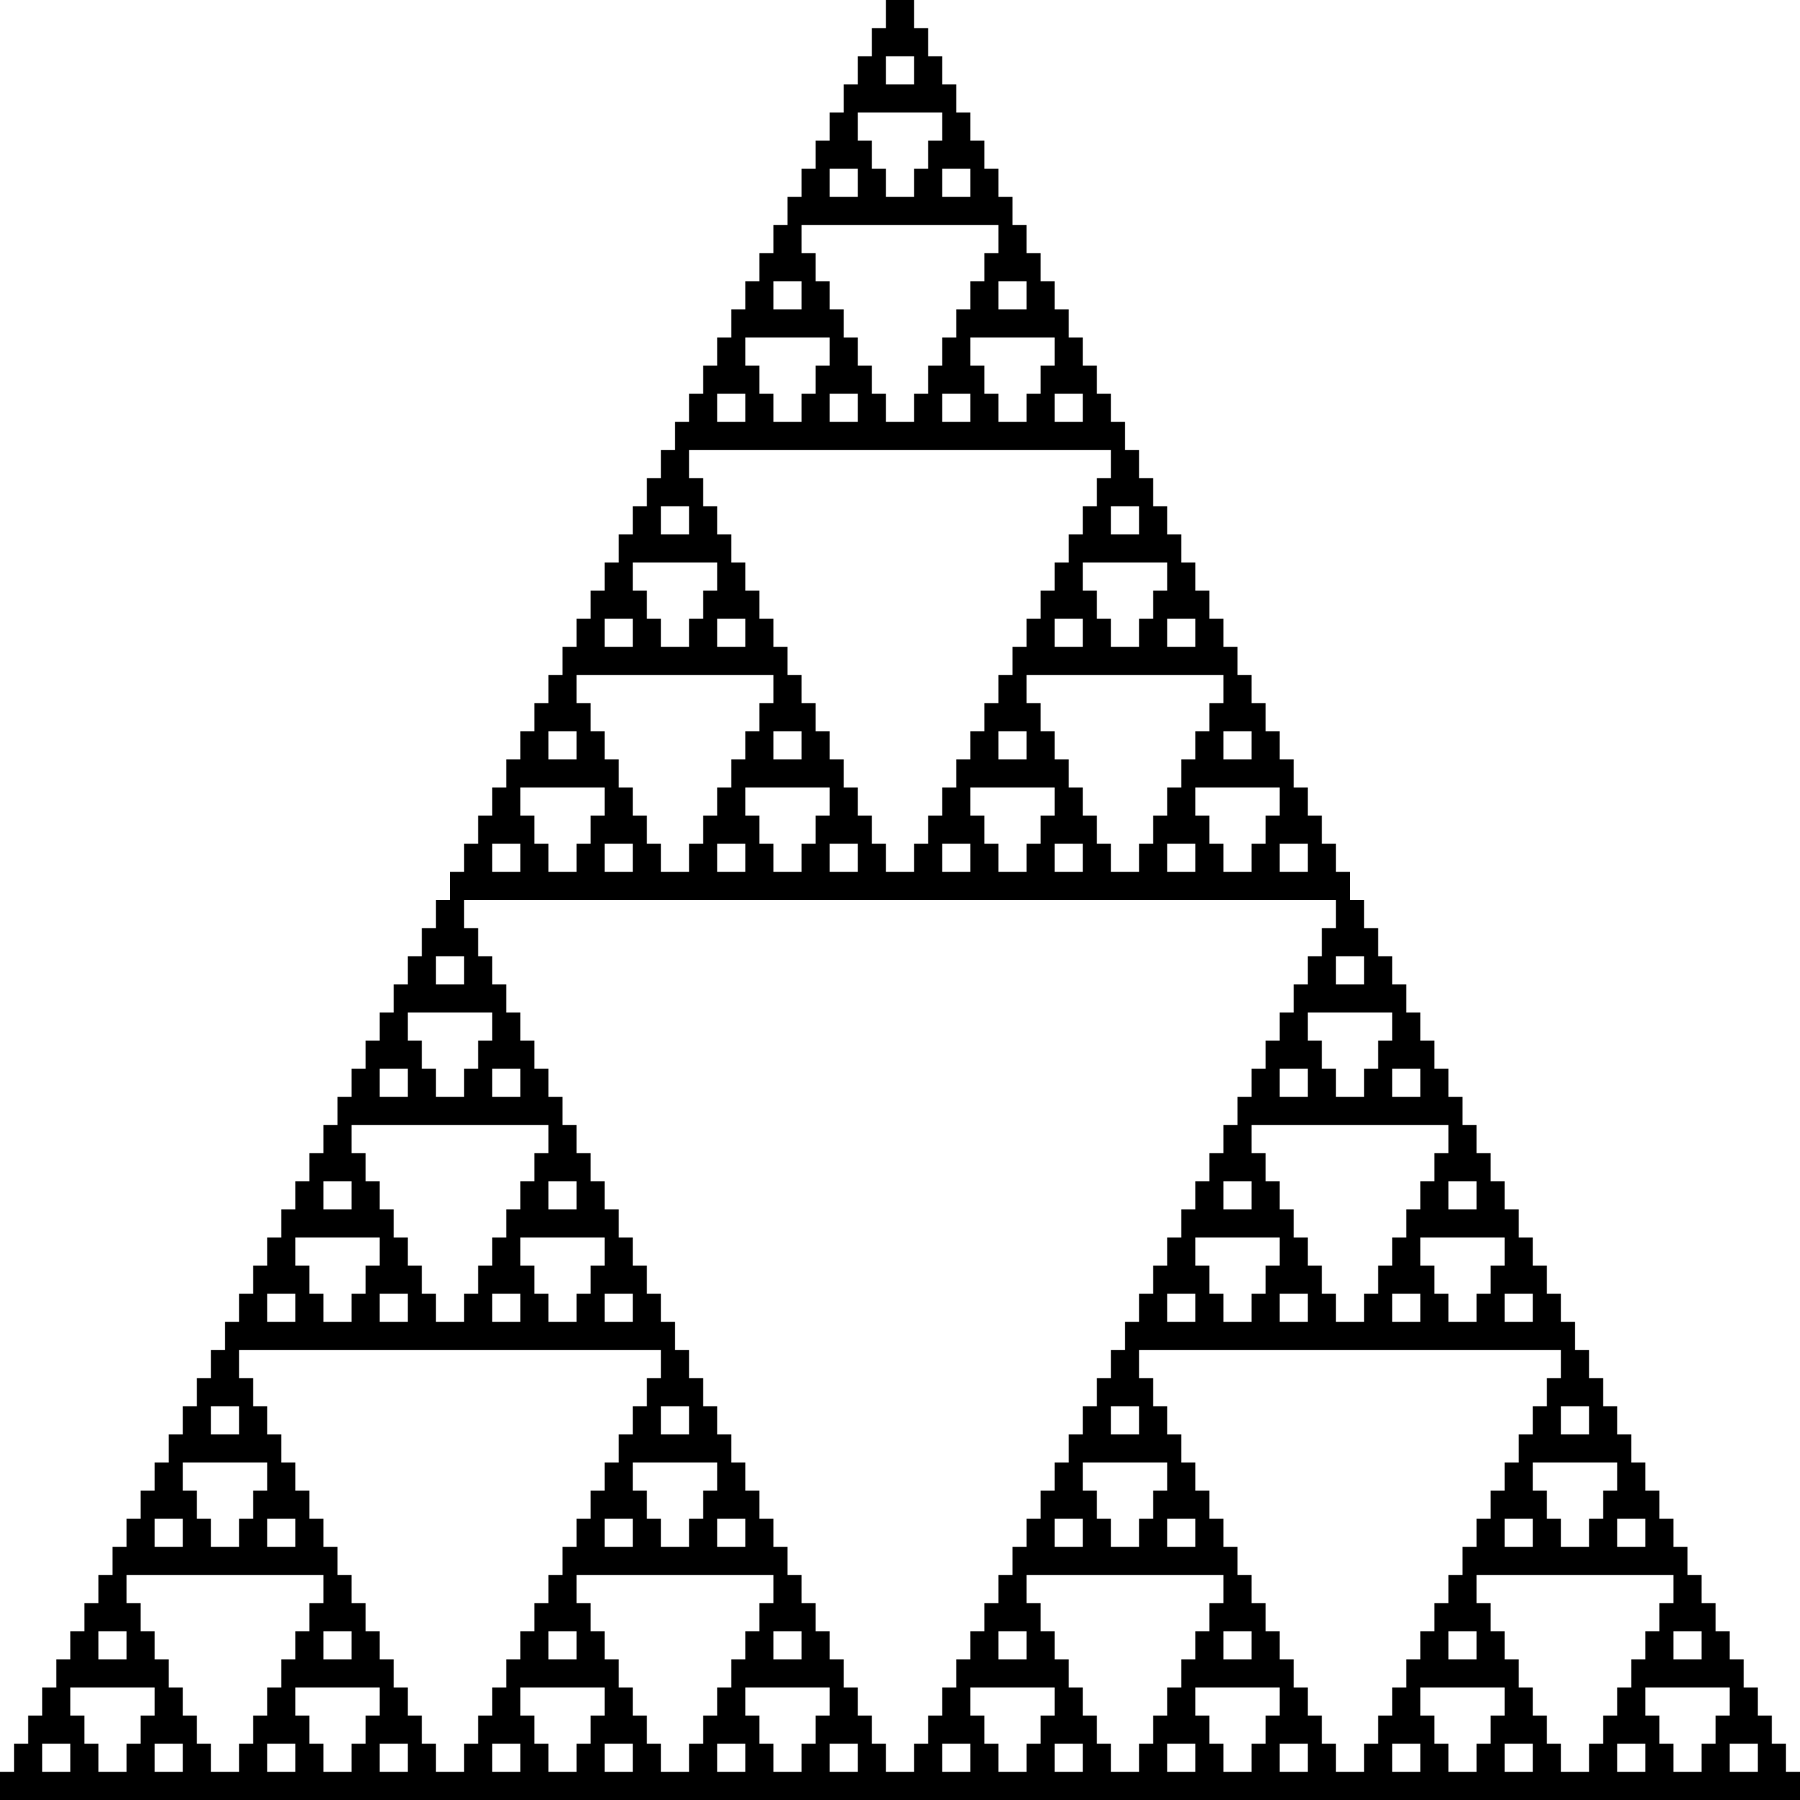
\includegraphics[width=0.25\textwidth]{papers/ifs/images/sierpinski6}}
	\caption{Konstruktion eines Sierpinski-Dreiecks mit einem Schwarzen Quadrat als Start\\
		(a) 1. Iteration (b) 2. Iteration (c) 3. Iteration (d) 5. Iteration}
	\label{ifs:sierpconst}
\end{figure}
Im Beispiel der Abbildung \ref{ifs:sierpconst} sehen wir, wie das Bild nach jeder Iteration dem Sierpinski-Dreieck ähnlicher wird.
Der Abstand zum Original wird immer kleiner, und konvergiert gegen null.

\subsection{Iterierte Funktionensysteme
\label{ifs:subsection:bonorum}}
In diesem Abschnitt wollen wir die Erkenntnis, wie wir aus einer beliebigen Menge ein Sierpinski-Dreieck generieren können, verallgemeinern.


$S_1,...,S_n$ sind Kontraktionen auf die Menge $D \subset \mathbb{R}^n$. Es gilt
\begin{align}
	|S_i(x) - S_i(y)| \leq c_i|x - y|
\end{align}
für jedes i mit einem $c_i < 1$. Dann existiert eine eindeutige kompakte Menge $F$ für die gilt
\begin{equation}
	F = \bigcup\limits_{i = 1}^{m} S_i(F)
\end{equation}
Weiter definieren wir die Transformation S auf kompakte Mengen ohne die leere Menge.
\begin{equation}
	S(E) = \bigcup\limits_{i = 1}^m S_i(E)
\end{equation}
Wird diese Transformation Iterativ ausgeführt, das heisst $S^0(E) = E, S^k(E) = S(S^{k-1}(E))$, und für jedes $i$ $S_i(E) \subset E$, gilt
\begin{equation}
	F = \bigcap\limits_{k = 1}^{\infty} S^k(E).
\end{equation}
In Worte gefasst bedeutet das, dass jede Gruppe von Kontraktionen iterativ ausgeführt, gegen eine eindeutige Menge konvergiert.
Diese Menge ist auch als Attraktor des IFS bekannt.
Dies für jede Startmenge, solange diese ihre Transformierten wieder beinhaltet.
Auf den Beweis wird verzichtet.
\subsection{Beispiel: Barnsley-Farn}
Der Barnsley-Farn, Abbildung \ref{ifs:farn}, ist ein Beispiel eines Fraktal, welches mit einem IFS generiert werden kann.
Wie man schnell erkennen kann, besteht der Farn aus Blättern, welche eine grosse Ähnlichkeit zum ganzen Farn haben.
\begin{align*}
	{S_1(x,y)}
	= 
	\begin{pmatrix}
		0 & 0 \\
		0 & 0.16 \\
	\end{pmatrix}
	\begin{pmatrix}
		x\\
		y\\
	\end{pmatrix}, \quad
	{S_2(x,y)}
	= 
	\begin{pmatrix}
		0.85 & 0.04 \\
		-0.04 & 0.85 \\
	\end{pmatrix}
	\begin{pmatrix}
		x\\
		y\\
	\end{pmatrix} 
	+
	\begin{pmatrix}
		0 \\
		1.6
	\end{pmatrix}\\
	{S_3(x,y)}
	= 
	\begin{pmatrix}
		0.2 & -0.26 \\
		0.23 & 0.22 \\
	\end{pmatrix}
	\begin{pmatrix}
		x\\
		y\\
	\end{pmatrix} 
	+
	\begin{pmatrix}
		0 \\
		1.6
	\end{pmatrix}, \quad
	{S_4(x,y)}
	= 
	\begin{pmatrix}
		-0.15 & 0.28 \\
		0.26 & 0.24 \\
	\end{pmatrix}
	\begin{pmatrix}
		x\\
		y\\
	\end{pmatrix} 
	+
	\begin{pmatrix}
		0 \\
		0.44
	\end{pmatrix}\\
\end{align*}
In der Abbildung \ref{ifs:farncolor} sehen wir die vier Transformationen farblich dargestellt.

$S_1$ erstellt den Stiel des Farnblattes (rot).
Die Transformation bildet das Gesamte Blatt auf die Y-Achse ab.
$S_2$ (grün) erstellt den Hauptteil des Farnes. 
Sie verkleinert und dreht das gesamte Bild und stellt es auf das Ende des Stiels aus $S_1$.
$S_3$ bildet das gesamte Blatt auf das blaue Teilblatt unten Links ab.
$S_4$ spiegelt das Blatt und bildet es auf das magentafarbene Teilblatt ab.  
\subsection{Chaosspiel}
Wir führen im Zusammenhang mit dem Barnsley-Farn \cite{ifs:barnsleyfern} noch eine weitere Methode ein, um ein IFS zu zeichnen.
Bis jetzt wurde immer davon gesprochen, die Transformationen auf die gesamte Menge anzuwenden.
Bei komplizierteren IFS welche viele Iterationen brauchen, bis man den Attraktor erkennen kann, ist diese Methode ziemlich rechenintensiv.
Eine Alternative ist das Chaosspiel \cite{ifs:chaos}. 
Bei dieser Methode werden die Transformationen nicht auf die Menge angewendet, sondern nur auf einen einzelnen Punkt.
Der Startpunkt kann dabei ein beliebiger Punkt in $E$ sein.
Es wird bei jedem Iterationsschritt nur eine Transformation, welche zufällig gewählt wurde, angewendet.
Da, wie wir beim Barnsley-Farn gut sehen, dass nicht jede Transformation gleich viel des Bildes ausmacht, werden diese beim Chaosspiel gewichtet.
Die Gewichtung erfolgt über den Anteil der Gesamtmasse.
Im Fall des Barnsley-Fern wird $S_1$ in $1\%$, $S_2$ in $85\%$ und $S_3 \& S_4$ in $7\%$ der Iterationen ausgeführt. 
\begin{figure}	
	\centering
	\makebox[\textwidth][c]{
		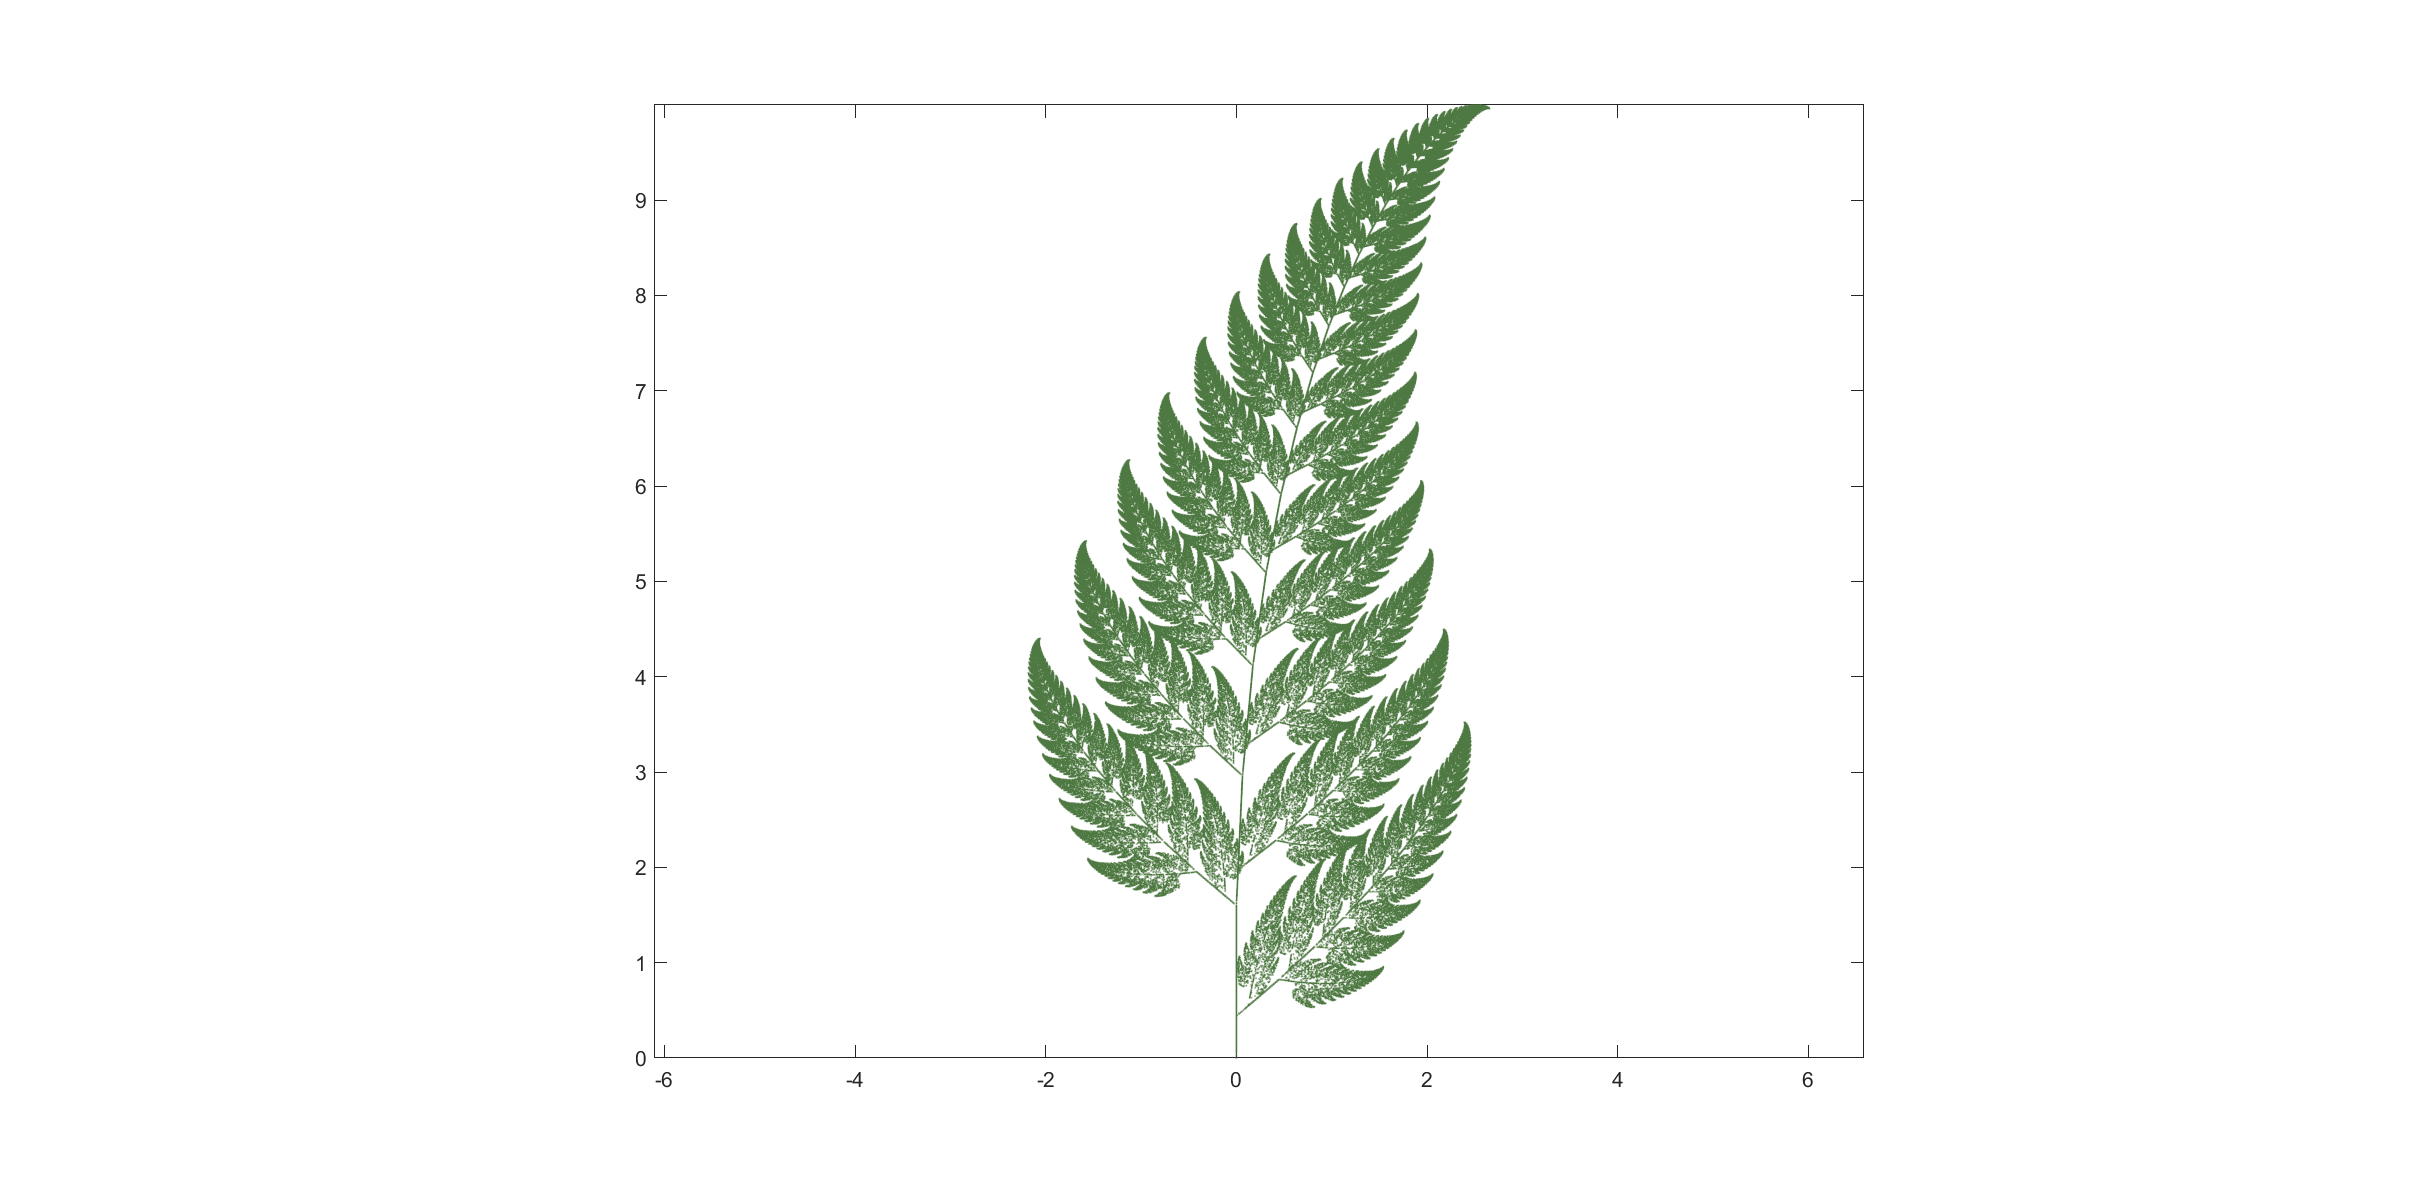
\includegraphics[width=1.4\textwidth]{papers/ifs/images/farn}}
	\caption{Barnsley-Farn}
	\label{ifs:farn}
\end{figure}
\begin{figure}
	\centering
	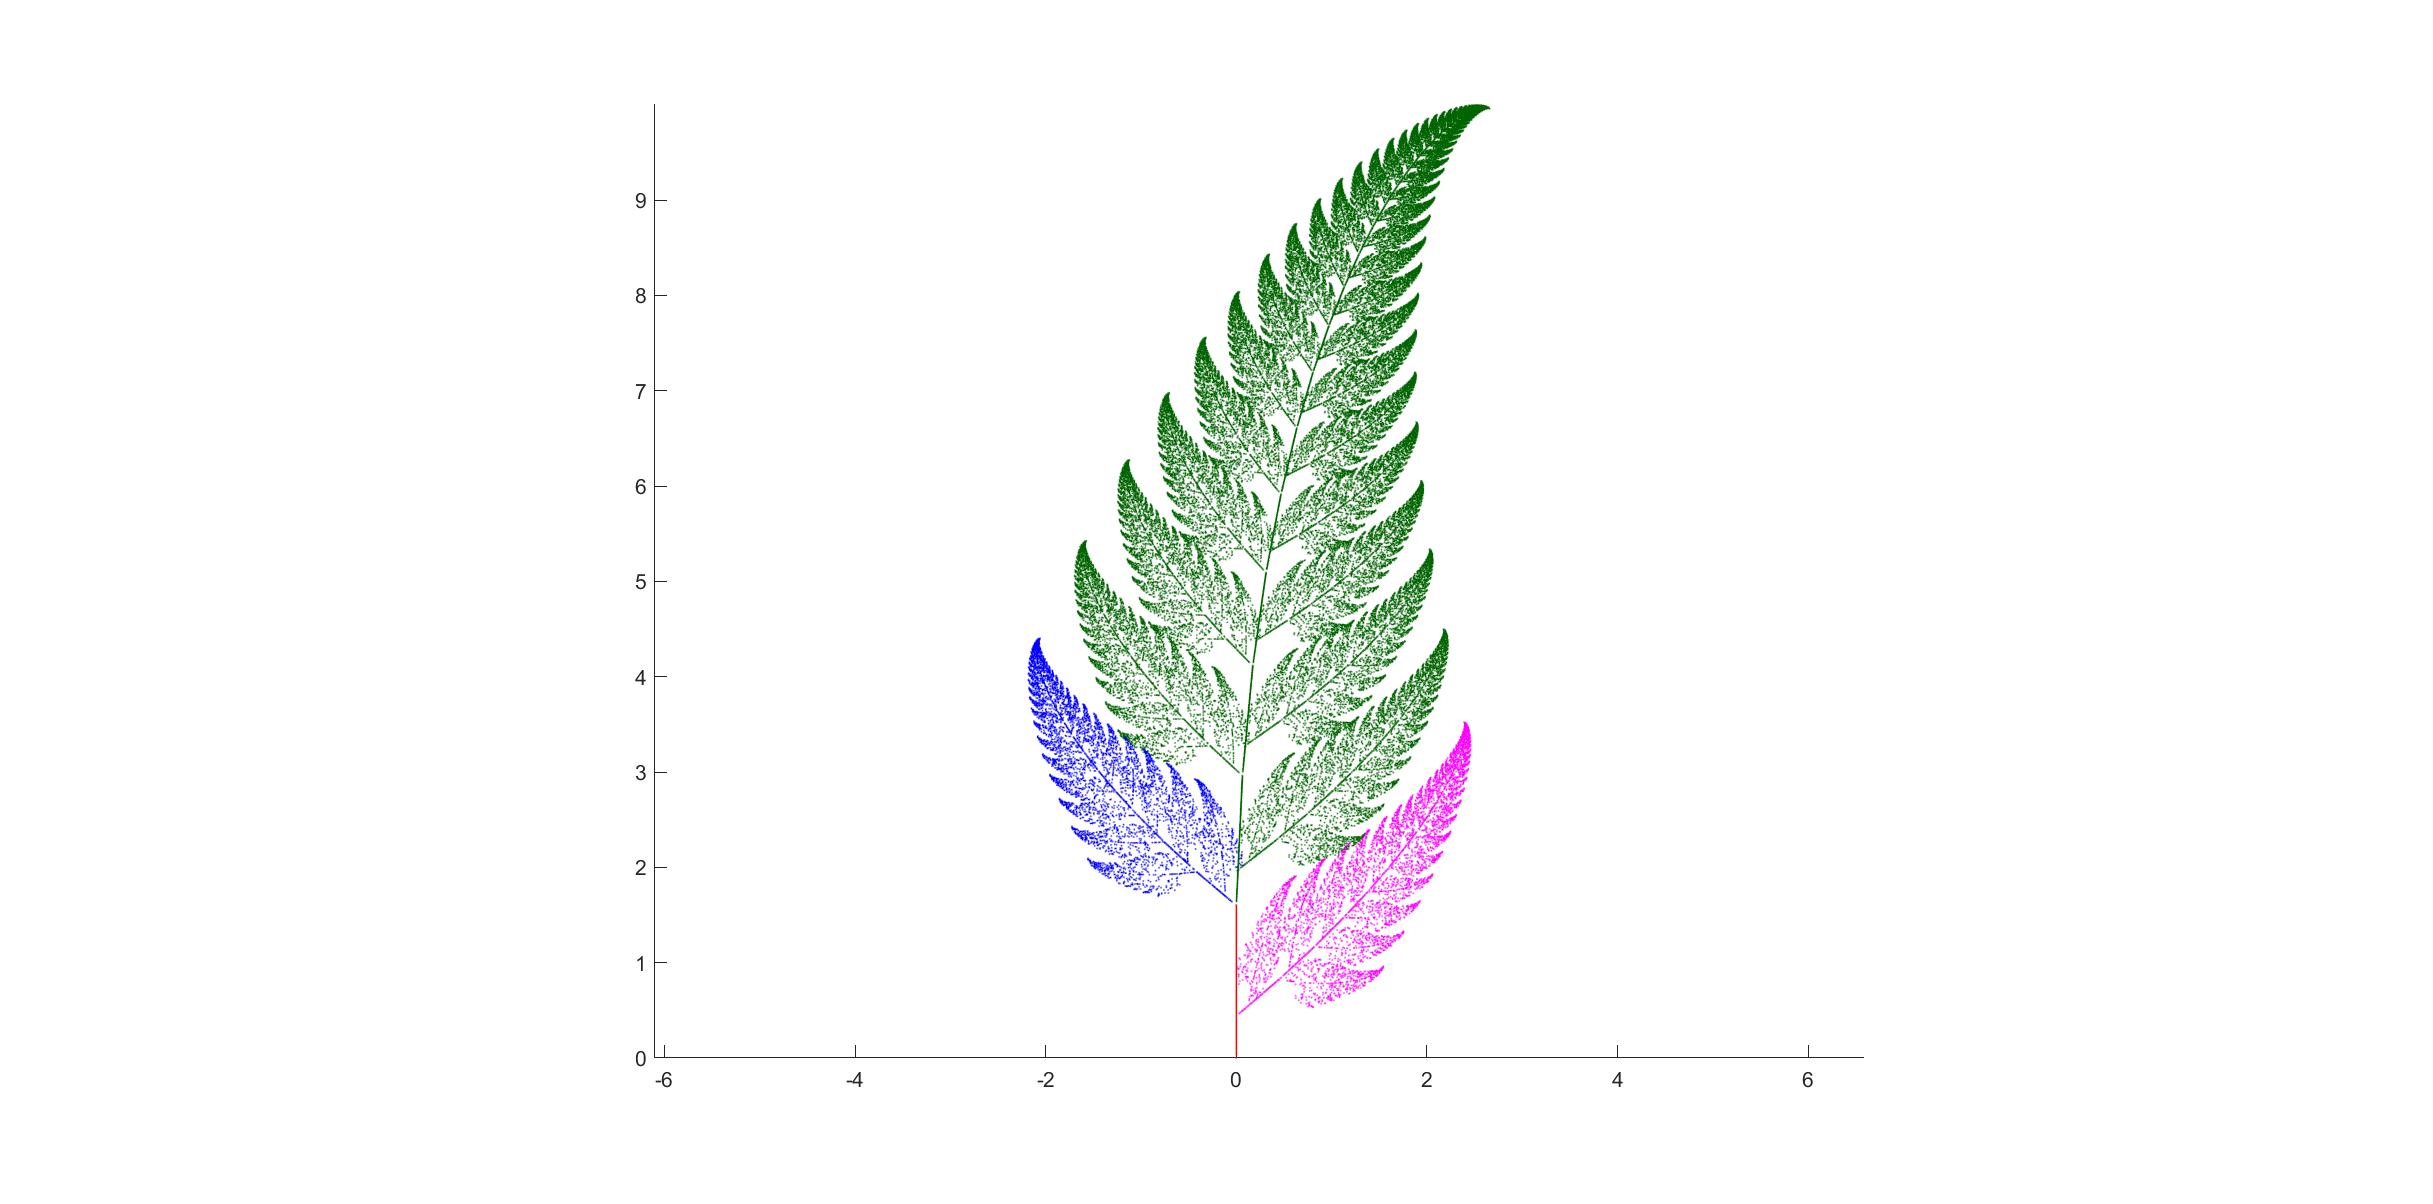
\includegraphics[width=0.7\textwidth]{papers/ifs/images/farncolor}
	\caption{Vier Transformationen des Barnsley-Farn}
	\label{ifs:farncolor}
\end{figure}
\begin{figure}	
	\centering
	\makebox[\textwidth][c]{
		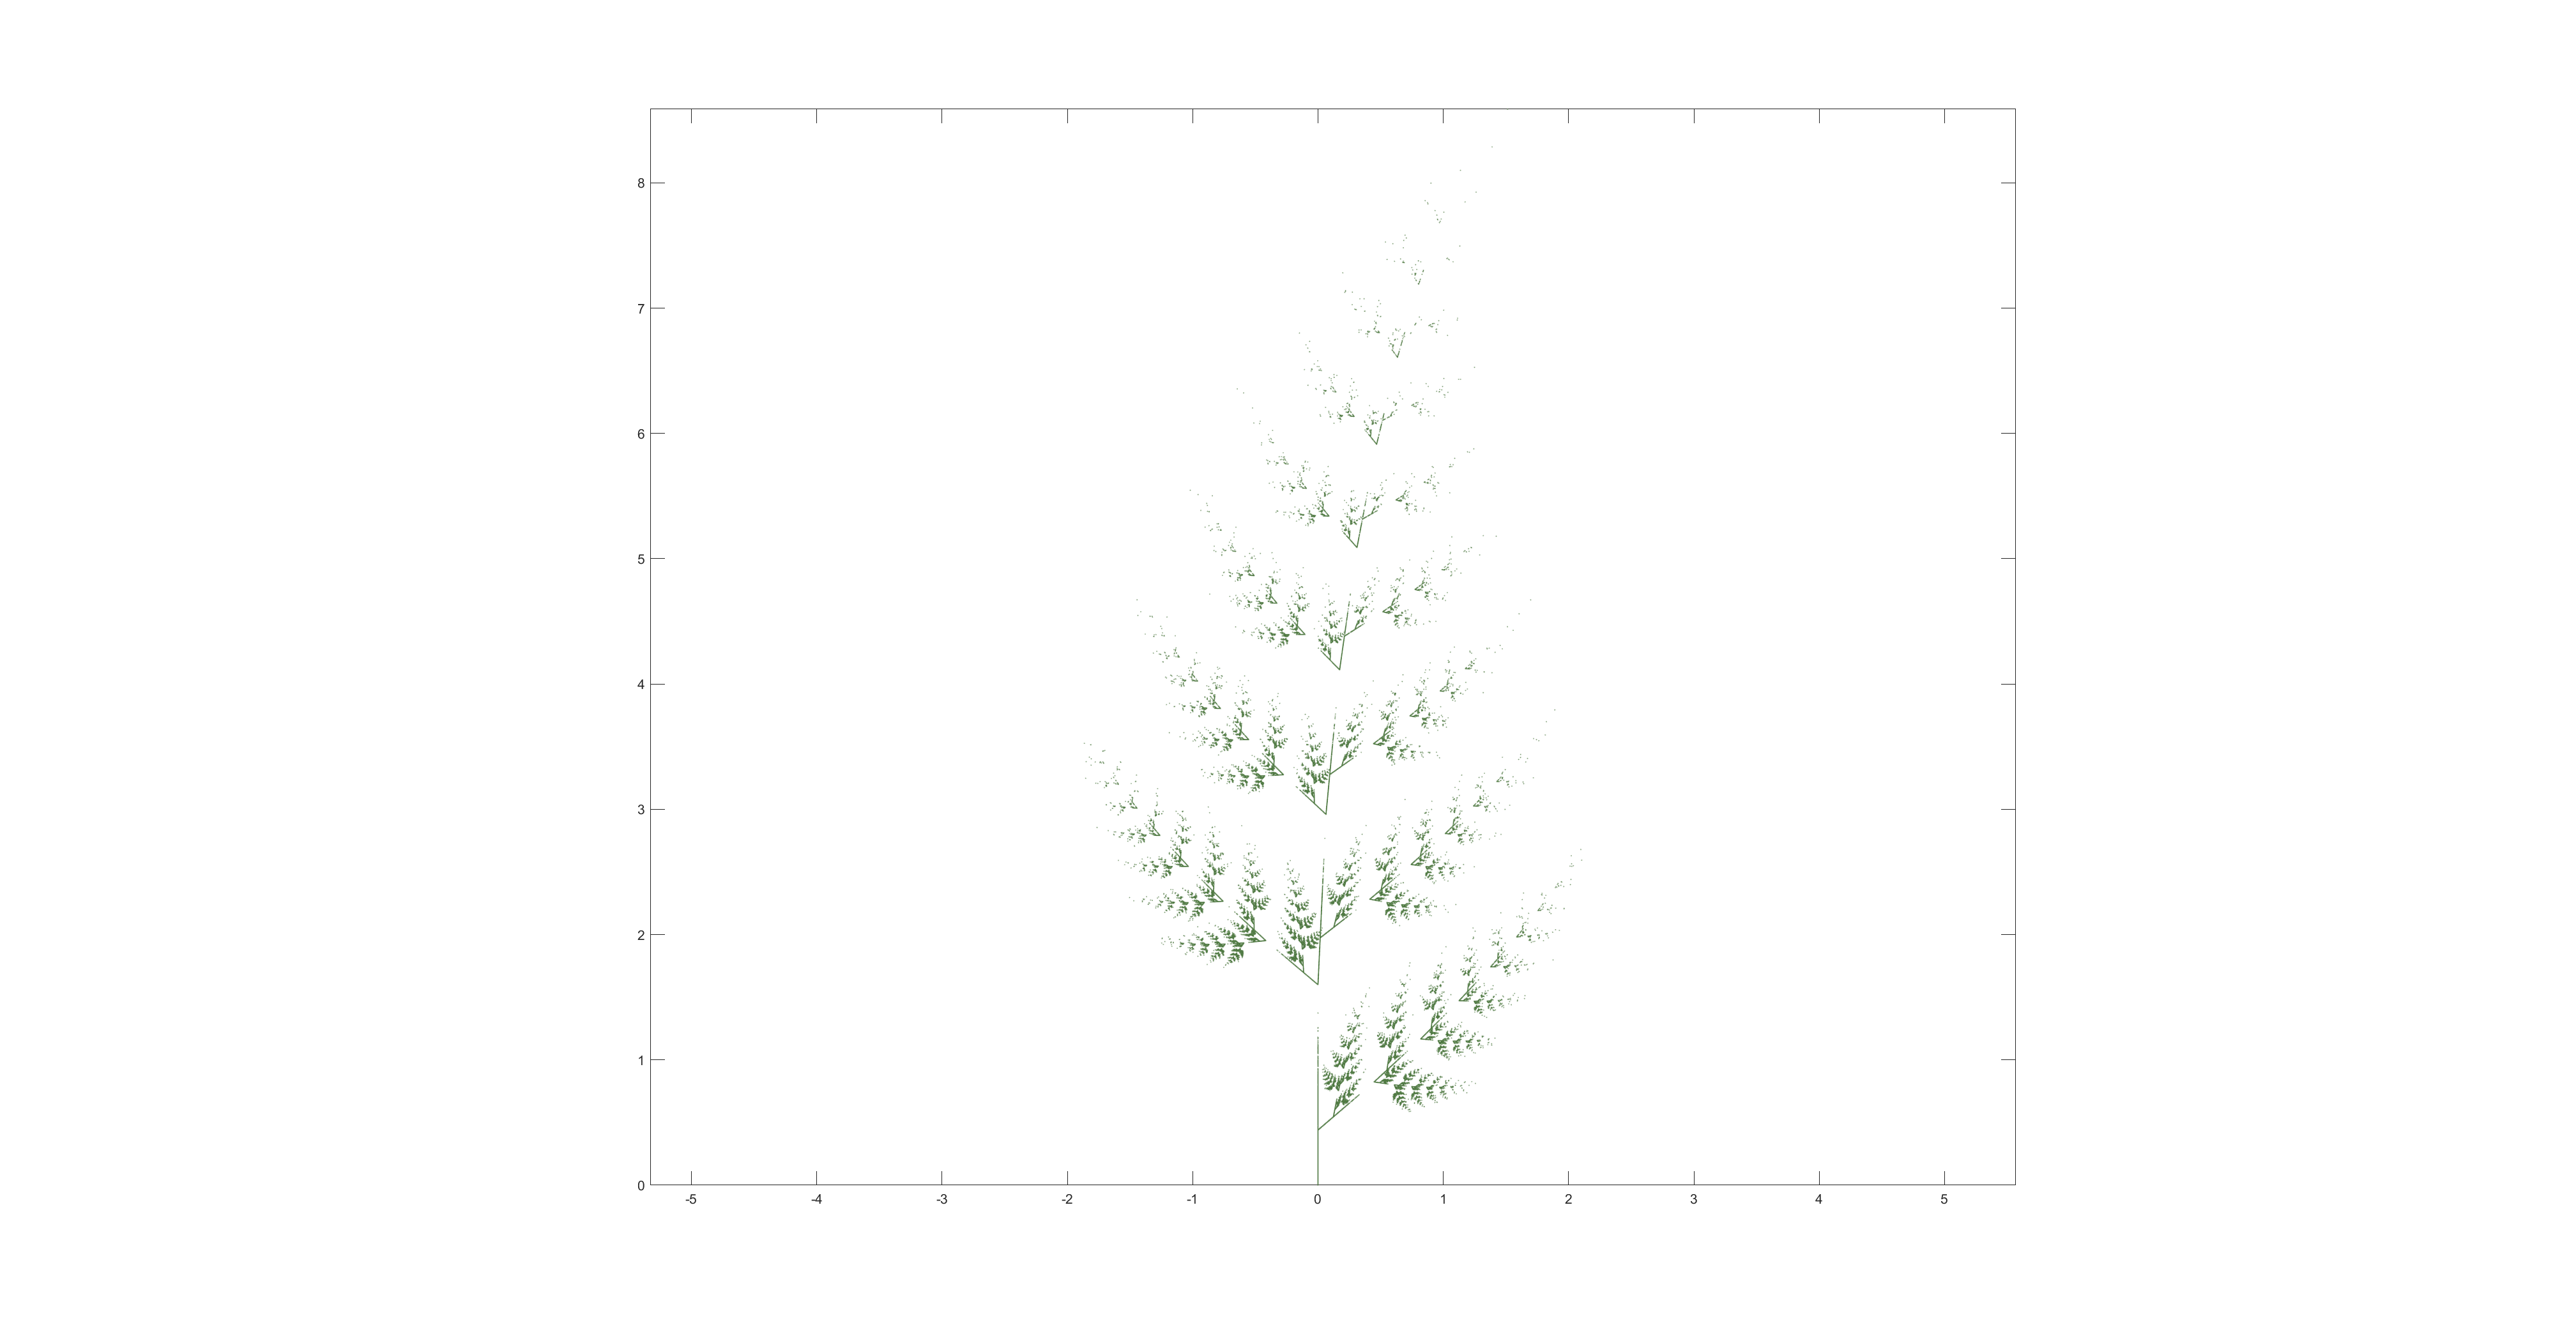
\includegraphics[width=1.4\textwidth]{papers/ifs/images/farnnotweight}}
	\caption{Chaosspiel ohne Gewichtung}
	\label{ifs:farnNoWeight}
\end{figure}

%
% teil3.tex -- Beispiel-File für Teil 3
%
% (c) 2020 Prof Dr Andreas Müller, Hochschule Rapperswil
%
\section{Der Munkres-Algorithmus oder die ungarische Methode
\label{munkres:section:teil3}}

Mit der ungarischen Methode können also Optimierungsprobleme gelöst
werden, die bei gewichteten Zuordnungen in bipartiten Graphen entstehen.
Mit ihr kann die eindeutige Zuordnung von Objekten aus zwei Gruppen so
optimiert werden, dass die Gesamtkosten minimiert werden bzw.~der
Gesamtgewinn maximiert werden kann.

\rhead{Ungarische Methode}

\subsection{Geschichte
\label{munkres:subsection:malorum}}
Die Ungarische Methode wurde 1955 von Harold Kuhn entwickelt und veröffentlicht.
\index{Kuhn, Harold}%
Der Name ``Ungarische Methode'' ergab sich, weil der Algorithmus
weitestgehend auf den früheren Arbeiten zweier ungarischer Mathematiker
basierte: Dénes Kőnig und Jenő Egerváry.
\index{Konig, Denes@Kőnig, Dénes}%
\index{Egerváry, Jenő}%
\index{Munkres, James}%
James Munkres überprüfte den Algorithmus im Jahr 1957 und stellte fest,
dass der Algorithmus (stark) polynomiell ist.
Seitdem ist der Algorithmus auch als Kuhn-Munkres- oder
Munkres-Zuordnungsalgorithmus bekannt.
\index{Kuhn-Munkres-Zuordnungsalgorithmus}%
\index{Munkres-Zuordnungsalgorithmus}%
Die Zeitkomplexität des ursprünglichen Algorithmus war $O(n^4)$,
später wurde zudem festgestellt, dass er modifiziert werden kann,
um eine  $O(n^3)$-Laufzeit zu erreichen.

\subsection{Besondere Leistung der Ungarischen Methode
\label{munkres:subsection:malorum}}
Die ungarische Methode ist ein kombinatorischer Optimierungsalgorithmus, der das Zuordnungsproblem
\index{Optimierungsalgorithmus, kombinatorisch}%
in polynomieller Zeit löst.
Der Begriff polynomielle Laufzeit bedeutet, dass die Laufzeit des Programms
\index{polynomielle Laufzeit}%
wie $n^2$, $n^3$, $n^4$, etc.~wächst und vernünftig skaliert. $n$ ist hierbei die ``Grösse'' des Problems.

\subsection{Unterschiedliche Anzahl von Quellen und Zielen
\label{munkres:subsection:malorum}}
Es gibt Fälle, in welchen das Ausgangsproblem keine quadratische Form besitzt.
Das ist z.~B.~dann der Fall, wenn drei Mitarbeiter vier verschiedene Eignungstests absolvieren müssen.
In diesem Fall wird in der Ungarischen Methode die Matrix künstlich mittels einer Dummy-Position zu einem Quadrat ergänzt.
Dummy-Positionen werden dann mit der größten vorhandenen Zahl aus der Matrix besetzt.
Beispielsweise wird eine $3\times 4$ zu einer $4\times 4$-Matrix.

\subsection{Beispiel eines händischen Verfahrens
\label{munkres:subsection:malorum}}
\begin{figure}
\centering
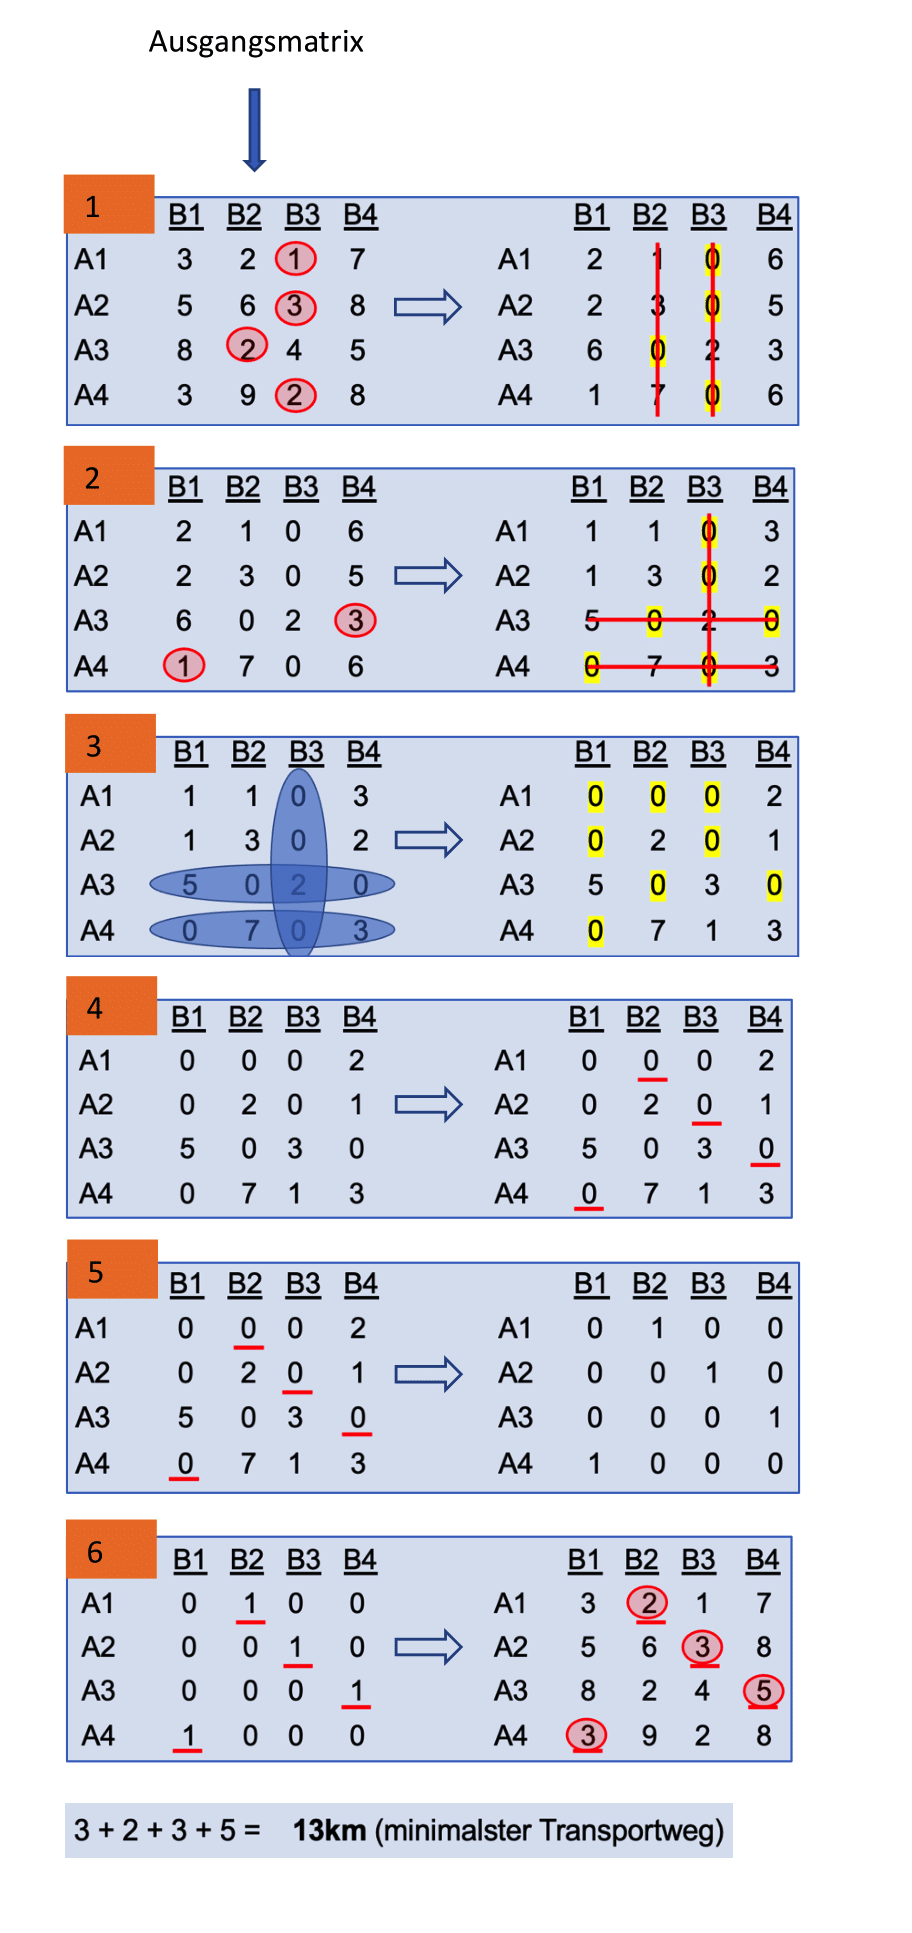
\includegraphics[width=8cm]{papers/munkres/figures/Ungarische_Methode_Beispiel.png}
\caption{Händisches Beispiel des Munkres Algorithmus, minimaler Transportweg.}
\label{munkres:Vr2}
\end{figure}

Die ungarische Methode kann in einem einfachen händischen Beispiel erläutert werden. Wir gehen von der Kostenmatrix $A$ aus. Diese Matrix wird in mehreren Schritten immer weiter reduziert. Anschliessend erfolgen mehrere Zuordnungen. Hierbei ist zu beachten, dass jede Zeile und jede Spalte immer genau eine eindeutige Zuordnung ergibt. Es gibt Situationen, in denen man nichts mehr tun muss, um eine optimale Zuordnung zu finden. Eine optimale Zuordnung ohne zusätzliche Kosten ist eine Auswahl genau eines Feldes in jeder Zeile und Spalte, welches 0 enthält. Das Ziel des Algorithmus ist also, die Matrix so zu ändern, dass genügend Nullen in der Matrix vorkommen. Es ist zudem wichtig, dass man nach jeder Modifikation der Matrix testet, ob man bereits eine Zuordnung machen kann, also genügend Nullen hat.
Das Vorgehen wird in den nachfolgenden Schritten 1--6 beschrieben und auch in der Abbildung 21.5 dargestellt.

\begin{enumerate}
\item Man beginnt mit der Zeilen-Reduktion. Pro Zeile eruiert man die kleinste Zahl. Diese kleinste Zahl, jeweils in rot markiert, wird bei allen anderen Ziffern in der jeweiligen Zeile subtrahiert. Mit dieser Subtraktion zieht man die unvermeidbaren Kosten ab, die man hat, um eine Baustelle zu erreichen. Man erkennt, dass die Nullen mit zwei Linien abdeckbar sind. Das heisst es gibt zwei Spalten bei denen noch keine Zuordnungen möglich sind. 

\item Auch im zweiten Schritt werden mittels der Spalten-Reduktion die unvermeidbaren Weg-Kosten abgezogen. Man zieht die kleinste Zahl, wiederum in rot markiert, in jeder Spalte von allen Zahlen in der Spalte ab.
Die Nullen können somit mit drei Linien abgedeckt werden. Im Idealfall hat die Matrix in jeder Zeile und Spalte bereits genügend viele Nullen, so dass man bereits eine Zuordnung ohne Mehrkosten machen kann. Dies ist jedoch noch nicht der Fall. Es sollen weitere Nullen in die Matrix hineingebracht werden.

\item Es bleiben jetzt einige Felder übrig, für die noch keine Zuordnung möglich ist. Die kleinste Ziffer wird dabei aus den noch nicht mit blau markierten Zahlen ausgewählt werden. Im Beispiel ist es die Zahl 1. Das Feld mit dem kleinsten Eintrag beinhaltet die Kosten, die unvermeidlich sind, wenn man für diese Felder auch noch eine Zuordnung machen will. Um neue Nullen zu bekommen, lagert man jetzt die Kosten auf die anderen Zeilen und Spalten um. Dies tut man, indem man in allen nicht abgedeckten Feldern die minimalen Kosten subtrahiert und in den blau markierten Kreuzungspunkten dazu addiert.
Dieser Schritt 3 muss so oft wiederholt werden, bis genügend viele Nullen in der Matrix vorhanden sind.

\item In Schritt 4 sollen jetzt möglichst viele Nullen markiert werden, welche freistehend sind.
Freistehend bedeutet, dass sowohl in der jeweiligen Zeile und Spalte keine andere markierte Null vorhanden ist.

\item Alle markierten Nullen werden jetzt in eine 1 umgewandelt. Die restlichen Ziffern in der Matrix, exklusiv die Einsen, sollen jetzt ignoriert und durch eine 0 ersetzt werden.

\item Zu guter Letzt werden überall wo eine 1 steht, die Zahlen aus der Ausgangsmatrix eingefügt. Nach Einsetzen der Zahlen können die in rot markierten Zahlen aufsummiert werden. Man erhält den minimalen Transportweg von total 13 Kilometer.
\end{enumerate}

\begin{figure}
\centering
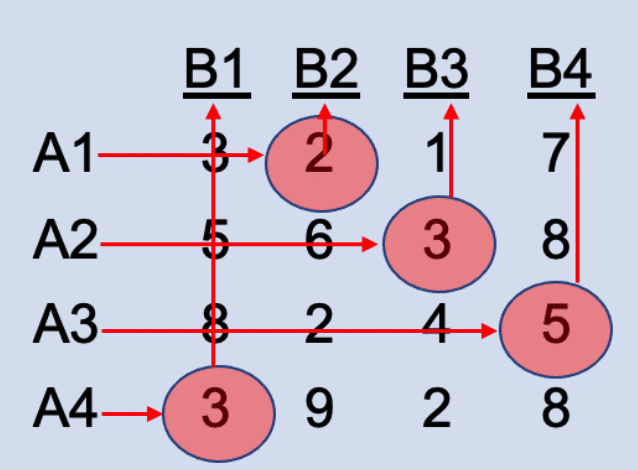
\includegraphics[width=3cm]{papers/munkres/figures/Ungarische_Methode_Beispiel_Zuw.png}
\caption{Händisches Beispiel des Munkres Algorithmus, Zuweisung der Kräne }
\label{munkres:Vr2}
\end{figure} 

\subsection{Zuordnung der Kräne
\label{munkres:subsection:malorum}}

Als Resultat des Munkres-Algorithmus werden in Abbildung 21.6 nebst dem minimalen Transportweg auch die optimale Zuweisung der Kräne auf die neuen Standorte ersichtlich.
Es können die folgenden Zuordnungen aus der Matrix abgelesen werden:
\begin{itemize}
\item Der Kran von Baustelle A1 soll zur Baustelle B2.
\item Der Kran von Baustelle A2 soll zur Baustelle B3.
\item Der Kran von Baustelle A3 soll zur Baustelle B4.
\item Der Kran von Baustelle A4 soll zur Baustelle B1.
\end{itemize}



% Michael
%
% teil1.tex -- Beispiel-File für das Paper
%
% (c) 2020 Prof Dr Andreas Müller, Hochschule Rapperswil
%
\section{Reed-Solomon in Endlichen Körpern
\label{reedsolomon:section:endlichekoerper}}
\rhead{Problemstellung}

\textcolor{red}{TODO: (warten auf den 1. Teil)}

Das Rechnen in endlichen Körpern bietet einige Vorteile:

\begin{itemize}
	\item Konkrete Zahlen: In endlichen Körpern gibt es weder rationale noch komplexe Zahlen. Zudem beschränken sich die möglichen Rechenoperationen auf das Addieren und Multiplizieren. Somit können wir nur ganze Zahlen als Resultat erhalten.
	
	\item Digitale Fehlerkorrektur: lässt sich nur in endlichen Körpern umsetzen. 
	
\end{itemize}

Um jetzt eine Nachricht in den endlichen Körpern zu konstruieren legen wir fest, dass diese Nachricht aus einem Nutzdatenteil und einem Fehlerkorrekturteil bestehen muss. Somit ist die zu übertragende Nachricht immer grösser als die Daten, die wir übertragen wollen. Zudem müssen wir einen Weg finden, den Fehlerkorrekturteil so aus den Nutzdaten zu berechnen, dass wir die Nutzdaten auf der Empfängerseite wieder rekonstruieren können, sollte es zu einer fehlerhaften Übertragung kommen.

Nun stellt sich die Frage, wie wir eine fehlerhafte Nachricht korrigieren können, ohne ihren ursprünglichen Inhalt zu kennen. Der Reed-Solomon-Code erzielt dies, indem aus dem Fehlerkorrekturteil ein sogenanntes ``Lokatorpolynom'' generiert werden kann. Dieses Polynom gibt dem Emfänger an, welche Stellen in der Nachricht feherhaft sind. 

%
% codebsp.tex -- Codierung eines Beispiels
%
% (c) 2021 Michael Steiner, Hochschule Rapperswil
%
\section{Codierung eines Beispiels
\label{reedsolomon:section:codebsp}}

Um die Funktionsweise eines Reed-Solomon-Codes besser zu verstehen, werden wir die einzelnen Probleme und ihre Lösungen anhand eines Beispiels betrachten.
Da wir in endlichen Körpern rechnen, werden wir zuerst solch einen Körper festlegen. Dabei müssen wir die Definition \ref{buch:endlichekoerper:def:galois-koerper} berücksichtigen, die besagt, dass nur Primzahlen für endliche Körper in Frage kommen.
Wir legen für unser Beispiel den endlichen Körper $\mathbb{F}_{q}$ mit $q = 11$ fest.
Zur Hilfestellung beim Rechnen in $\mathbb{F}_{11}$ können die beiden Tabellen \ref{reedsolomon:subsection:adtab} und \ref{reedsolomon:subsection:mptab} hinzugezogen werden. Diese Tabellen enthalten die Resultate der arithmetischen Operationen im Körper $\mathbb{F}_{11}$, die durchgeführt werden können.
Aus der Definition der endlichen Körper (ersichtlich auch in den Tabellen) folgt, dass uns nur die Zahlen \[\mathbb{F}_{11} = \{0,1,2,3,4,5,6,7,8,9,10\}\] zur Verfügung stehen und somit $11 = 0$ gelten muss.

\rhead{Codierung eines Beispiels}
% OLD TEXT
%Alle folgenden Berechnungen wurden mit den beiden Restetabellen \ref{reedsolomon:subsection:adtab} und \ref{reedsolomon:subsection:mptab} durchgeführt.
%Aus den Tabellen folgt auch, dass uns nur die Zahlen \[\mathbb{F}_{11} = \{0,1,2,3,4,5,6,7,8,9,10\}\] zur Verfügung stehen.

% die beiden Restetabellen von F_11
%%
% restetabelle1.tex -- Restetabelle von F_11: Addition
%
% (c) 2021 Michael Steiner, Hochschule Rapperswil
%

% alternatives design
%\begin{figure}
%\begin{center}
%\begin{tabular}{|>{$}c<{$}|>{$}c<{$}>{$}c<{$}>{$}c<{$}>{$}c<{$}>{$}c<{$}>{$}c<{$}>{$}c<{$}>{$}c<{$}>{$}c<{$}>{$}c<{$}>{$}c<{$}|}
%\hline
%+&0&1&2&3&4&5&6&7&8&9&10\\
%\hline
%0&0&1&2&3&4&5&6&7&8&9&10\\
%1&1&2&3&4&5&6&7&8&9&10&0\\
%2&2&3&4&5&6&7&8&9&10&0&1\\
%3&3&4&5&6&7&8&9&10&0&1&2\\
%4&4&5&6&7&8&9&10&0&1&2&3\\
%5&5&6&7&8&9&10&0&1&2&3&4\\
%6&6&7&8&9&10&0&1&2&3&4&5\\
%7&7&8&9&10&0&1&2&3&4&5&6\\
%8&8&9&10&0&1&2&3&4&5&6&7\\
%9&9&10&0&1&2&3&4&5&6&7&8\\
%10&10&0&1&2&3&4&5&6&7&8&9\\
%\hline
%\end{tabular}
%\end{center}
%\end{figure}

\begin{center}

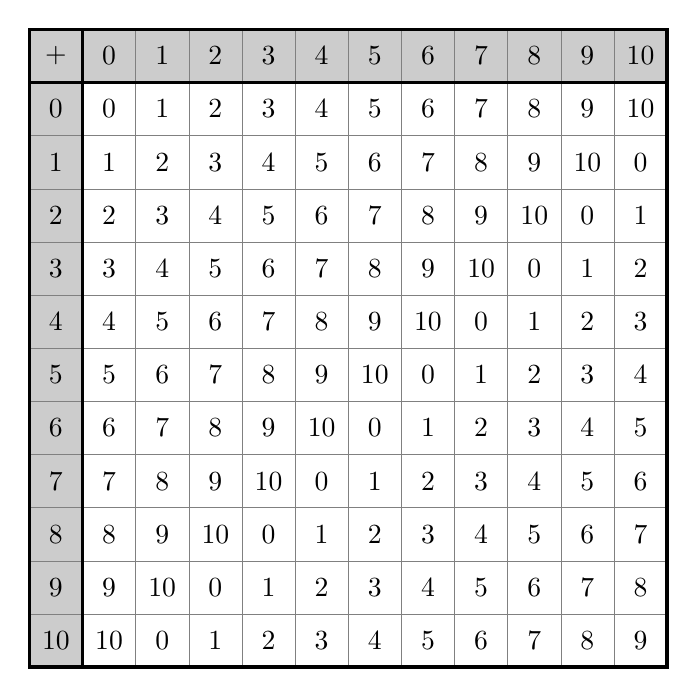
\begin{tikzpicture}[>=latex,thick,scale=0.45]
\fill[color=gray!40] (0,0) rectangle (18,-1.5);
\fill[color=gray!40] (0,0) rectangle (1.5,-18);	
\draw[step = 1.5, gray,very thin] (0,0) grid (18,-18);
\draw[very thick] (0,0) rectangle (18,-18);
\draw[very thick] (0,-1.5) -- (18,-1.5);
\draw[very thick] (1.5,0) -- (1.5,-18);
\node at (0.75,-0.75) {$+$};
\foreach \x in {0,...,10}
	\node at (2.25+\x*1.5,-0.75) {$\x$};
\foreach \y in {0,...,10}
	\node at (0.75,-2.25+\y*-1.5) {$\y$};
% Row 0
\node at ( 2.25,-2.25) {$0$};
\node at ( 3.75,-2.25) {$1$};
\node at ( 5.25,-2.25) {$2$};
\node at ( 6.75,-2.25) {$3$};
\node at ( 8.25,-2.25) {$4$};
\node at ( 9.75,-2.25) {$5$};
\node at (11.25,-2.25) {$6$};
\node at (12.75,-2.25) {$7$};
\node at (14.25,-2.25) {$8$};
\node at (15.75,-2.25) {$9$};
\node at (17.25,-2.25) {$10$};
% Row 1
\node at ( 2.25,-3.75) {$1$};
\node at ( 3.75,-3.75) {$2$};
\node at ( 5.25,-3.75) {$3$};
\node at ( 6.75,-3.75) {$4$};
\node at ( 8.25,-3.75) {$5$};
\node at ( 9.75,-3.75) {$6$};
\node at (11.25,-3.75) {$7$};
\node at (12.75,-3.75) {$8$};
\node at (14.25,-3.75) {$9$};
\node at (15.75,-3.75) {$10$};
\node at (17.25,-3.75) {$0$};
% Row 2
\node at ( 2.25,-5.25) {$2$};
\node at ( 3.75,-5.25) {$3$};
\node at ( 5.25,-5.25) {$4$};
\node at ( 6.75,-5.25) {$5$};
\node at ( 8.25,-5.25) {$6$};
\node at ( 9.75,-5.25) {$7$};
\node at (11.25,-5.25) {$8$};
\node at (12.75,-5.25) {$9$};
\node at (14.25,-5.25) {$10$};
\node at (15.75,-5.25) {$0$};
\node at (17.25,-5.25) {$1$};
% Row 3
\node at ( 2.25,-6.75) {$3$};
\node at ( 3.75,-6.75) {$4$};
\node at ( 5.25,-6.75) {$5$};
\node at ( 6.75,-6.75) {$6$};
\node at ( 8.25,-6.75) {$7$};
\node at ( 9.75,-6.75) {$8$};
\node at (11.25,-6.75) {$9$};
\node at (12.75,-6.75) {$10$};
\node at (14.25,-6.75) {$0$};
\node at (15.75,-6.75) {$1$};
\node at (17.25,-6.75) {$2$};
% Row 4
\node at ( 2.25,-8.25) {$4$};
\node at ( 3.75,-8.25) {$5$};
\node at ( 5.25,-8.25) {$6$};
\node at ( 6.75,-8.25) {$7$};
\node at ( 8.25,-8.25) {$8$};
\node at ( 9.75,-8.25) {$9$};
\node at (11.25,-8.25) {$10$};
\node at (12.75,-8.25) {$0$};
\node at (14.25,-8.25) {$1$};
\node at (15.75,-8.25) {$2$};
\node at (17.25,-8.25) {$3$};
% Row 5
\node at ( 2.25,-9.75) {$5$};
\node at ( 3.75,-9.75) {$6$};
\node at ( 5.25,-9.75) {$7$};
\node at ( 6.75,-9.75) {$8$};
\node at ( 8.25,-9.75) {$9$};
\node at ( 9.75,-9.75) {$10$};
\node at (11.25,-9.75) {$0$};
\node at (12.75,-9.75) {$1$};
\node at (14.25,-9.75) {$2$};
\node at (15.75,-9.75) {$3$};
\node at (17.25,-9.75) {$4$};
% Row 6
\node at ( 2.25,-11.25) {$6$};
\node at ( 3.75,-11.25) {$7$};
\node at ( 5.25,-11.25) {$8$};
\node at ( 6.75,-11.25) {$9$};
\node at ( 8.25,-11.25) {$10$};
\node at ( 9.75,-11.25) {$0$};
\node at (11.25,-11.25) {$1$};
\node at (12.75,-11.25) {$2$};
\node at (14.25,-11.25) {$3$};
\node at (15.75,-11.25) {$4$};
\node at (17.25,-11.25) {$5$};
% Row 7
\node at ( 2.25,-12.75) {$7$};
\node at ( 3.75,-12.75) {$8$};
\node at ( 5.25,-12.75) {$9$};
\node at ( 6.75,-12.75) {$10$};
\node at ( 8.25,-12.75) {$0$};
\node at ( 9.75,-12.75) {$1$};
\node at (11.25,-12.75) {$2$};
\node at (12.75,-12.75) {$3$};
\node at (14.25,-12.75) {$4$};
\node at (15.75,-12.75) {$5$};
\node at (17.25,-12.75) {$6$};
% Row 8
\node at ( 2.25,-14.25) {$8$};
\node at ( 3.75,-14.25) {$9$};
\node at ( 5.25,-14.25) {$10$};
\node at ( 6.75,-14.25) {$0$};
\node at ( 8.25,-14.25) {$1$};
\node at ( 9.75,-14.25) {$2$};
\node at (11.25,-14.25) {$3$};
\node at (12.75,-14.25) {$4$};
\node at (14.25,-14.25) {$5$};
\node at (15.75,-14.25) {$6$};
\node at (17.25,-14.25) {$7$};
% Row 9
\node at ( 2.25,-15.75) {$9$};
\node at ( 3.75,-15.75) {$10$};
\node at ( 5.25,-15.75) {$0$};
\node at ( 6.75,-15.75) {$1$};
\node at ( 8.25,-15.75) {$2$};
\node at ( 9.75,-15.75) {$3$};
\node at (11.25,-15.75) {$4$};
\node at (12.75,-15.75) {$5$};
\node at (14.25,-15.75) {$6$};
\node at (15.75,-15.75) {$7$};
\node at (17.25,-15.75) {$8$};
% Row 10
\node at ( 2.25,-17.25) {$10$};
\node at ( 3.75,-17.25) {$0$};
\node at ( 5.25,-17.25) {$1$};
\node at ( 6.75,-17.25) {$2$};
\node at ( 8.25,-17.25) {$3$};
\node at ( 9.75,-17.25) {$4$};
\node at (11.25,-17.25) {$5$};
\node at (12.75,-17.25) {$6$};
\node at (14.25,-17.25) {$7$};
\node at (15.75,-17.25) {$8$};
\node at (17.25,-17.25) {$9$};
\end{tikzpicture}

\end{center}

%% created by Michael Steiner
%
% Restetabelle von F_11: Multiplikation

% alternatives design
%\begin{figure}
%\begin{center}
%\begin{tabular}{|>{$}c<{$}|>{$}c<{$}>{$}c<{$}>{$}c<{$}>{$}c<{$}>{$}c<{$}>{$}c<{$}>{$}c<{$}>{$}c<{$}>{$}c<{$}>{$}c<{$}>{$}c<{$}|}
%\hline
%\cdot&0&1&2&3&4&5&6&7&8&9&10\\
%\hline
%0&0&0&0&0&0&0&0&0&0&0&0\\
%1&0&1&2&3&4&5&6&7&8&9&10\\
%2&0&2&4&6&8&10&1&3&5&7&9\\
%3&0&3&6&9&1&4&7&10&2&5&8\\
%4&0&4&8&1&5&9&2&6&10&3&7\\
%5&0&5&10&4&9&3&8&2&7&1&6\\
%6&0&6&1&7&2&8&3&9&4&10&5\\
%7&0&7&3&10&6&2&9&5&1&8&4\\
%8&0&8&5&2&10&7&4&1&9&6&3\\
%9&0&9&7&5&3&1&10&8&6&4&2\\
%10&0&10&9&8&7&6&5&4&3&2&1\\
%\hline
%\end{tabular}
%\end{center}
%\end{figure}

\begin{center}
	
	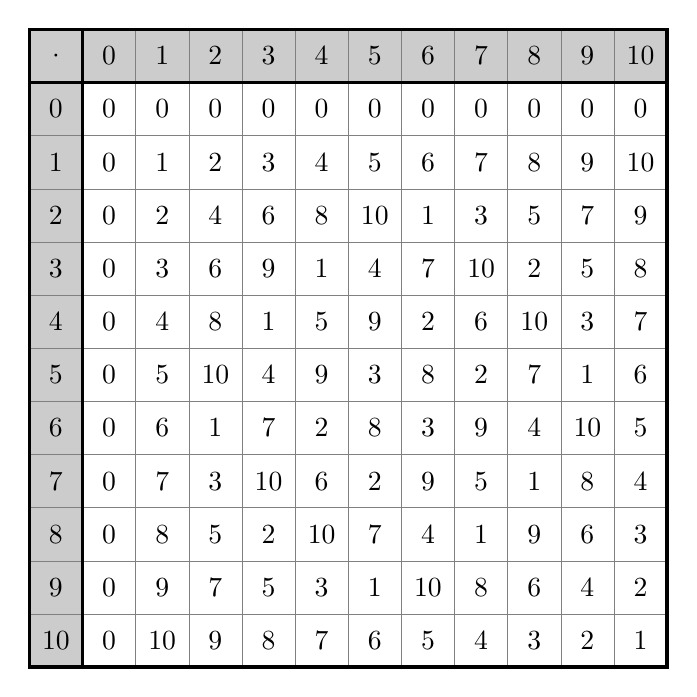
\begin{tikzpicture}[>=latex,thick,scale=0.45]
		\fill[color=gray!40] (0,0) rectangle (18,-1.5);
		\fill[color=gray!40] (0,0) rectangle (1.5,-18);	
		\draw[step = 1.5, gray,very thin] (0,0) grid (18,-18);
		\draw[very thick] (0,0) rectangle (18,-18);
		\draw[very thick] (0,-1.5) -- (18,-1.5);
		\draw[very thick] (1.5,0) -- (1.5,-18);
		\node at (0.75,-0.75) {$\cdot$};
		\foreach \x in {0,...,10}
		\node at (2.25+\x*1.5,-0.75) {$\x$};
		\foreach \y in {0,...,10}
		\node at (0.75,-2.25+\y*-1.5) {$\y$};
		% Row 0
		\node at ( 2.25,-2.25) {$0$};
		\node at ( 3.75,-2.25) {$0$};
		\node at ( 5.25,-2.25) {$0$};
		\node at ( 6.75,-2.25) {$0$};
		\node at ( 8.25,-2.25) {$0$};
		\node at ( 9.75,-2.25) {$0$};
		\node at (11.25,-2.25) {$0$};
		\node at (12.75,-2.25) {$0$};
		\node at (14.25,-2.25) {$0$};
		\node at (15.75,-2.25) {$0$};
		\node at (17.25,-2.25) {$0$};
		% Row 1
		\node at ( 2.25,-3.75) {$0$};
		\node at ( 3.75,-3.75) {$1$};
		\node at ( 5.25,-3.75) {$2$};
		\node at ( 6.75,-3.75) {$3$};
		\node at ( 8.25,-3.75) {$4$};
		\node at ( 9.75,-3.75) {$5$};
		\node at (11.25,-3.75) {$6$};
		\node at (12.75,-3.75) {$7$};
		\node at (14.25,-3.75) {$8$};
		\node at (15.75,-3.75) {$9$};
		\node at (17.25,-3.75) {$10$};
		% Row 2
		\node at ( 2.25,-5.25) {$0$};
		\node at ( 3.75,-5.25) {$2$};
		\node at ( 5.25,-5.25) {$4$};
		\node at ( 6.75,-5.25) {$6$};
		\node at ( 8.25,-5.25) {$8$};
		\node at ( 9.75,-5.25) {$10$};
		\node at (11.25,-5.25) {$1$};
		\node at (12.75,-5.25) {$3$};
		\node at (14.25,-5.25) {$5$};
		\node at (15.75,-5.25) {$7$};
		\node at (17.25,-5.25) {$9$};
		% Row 3
		\node at ( 2.25,-6.75) {$0$};
		\node at ( 3.75,-6.75) {$3$};
		\node at ( 5.25,-6.75) {$6$};
		\node at ( 6.75,-6.75) {$9$};
		\node at ( 8.25,-6.75) {$1$};
		\node at ( 9.75,-6.75) {$4$};
		\node at (11.25,-6.75) {$7$};
		\node at (12.75,-6.75) {$10$};
		\node at (14.25,-6.75) {$2$};
		\node at (15.75,-6.75) {$5$};
		\node at (17.25,-6.75) {$8$};
		% Row 4
		\node at ( 2.25,-8.25) {$0$};
		\node at ( 3.75,-8.25) {$4$};
		\node at ( 5.25,-8.25) {$8$};
		\node at ( 6.75,-8.25) {$1$};
		\node at ( 8.25,-8.25) {$5$};
		\node at ( 9.75,-8.25) {$9$};
		\node at (11.25,-8.25) {$2$};
		\node at (12.75,-8.25) {$6$};
		\node at (14.25,-8.25) {$10$};
		\node at (15.75,-8.25) {$3$};
		\node at (17.25,-8.25) {$7$};
		% Row 5
		\node at ( 2.25,-9.75) {$0$};
		\node at ( 3.75,-9.75) {$5$};
		\node at ( 5.25,-9.75) {$10$};
		\node at ( 6.75,-9.75) {$4$};
		\node at ( 8.25,-9.75) {$9$};
		\node at ( 9.75,-9.75) {$3$};
		\node at (11.25,-9.75) {$8$};
		\node at (12.75,-9.75) {$2$};
		\node at (14.25,-9.75) {$7$};
		\node at (15.75,-9.75) {$1$};
		\node at (17.25,-9.75) {$6$};
		% Row 6
		\node at ( 2.25,-11.25) {$0$};
		\node at ( 3.75,-11.25) {$6$};
		\node at ( 5.25,-11.25) {$1$};
		\node at ( 6.75,-11.25) {$7$};
		\node at ( 8.25,-11.25) {$2$};
		\node at ( 9.75,-11.25) {$8$};
		\node at (11.25,-11.25) {$3$};
		\node at (12.75,-11.25) {$9$};
		\node at (14.25,-11.25) {$4$};
		\node at (15.75,-11.25) {$10$};
		\node at (17.25,-11.25) {$5$};
		% Row 7
		\node at ( 2.25,-12.75) {$0$};
		\node at ( 3.75,-12.75) {$7$};
		\node at ( 5.25,-12.75) {$3$};
		\node at ( 6.75,-12.75) {$10$};
		\node at ( 8.25,-12.75) {$6$};
		\node at ( 9.75,-12.75) {$2$};
		\node at (11.25,-12.75) {$9$};
		\node at (12.75,-12.75) {$5$};
		\node at (14.25,-12.75) {$1$};
		\node at (15.75,-12.75) {$8$};
		\node at (17.25,-12.75) {$4$};
		% Row 8
		\node at ( 2.25,-14.25) {$0$};
		\node at ( 3.75,-14.25) {$8$};
		\node at ( 5.25,-14.25) {$5$};
		\node at ( 6.75,-14.25) {$2$};
		\node at ( 8.25,-14.25) {$10$};
		\node at ( 9.75,-14.25) {$7$};
		\node at (11.25,-14.25) {$4$};
		\node at (12.75,-14.25) {$1$};
		\node at (14.25,-14.25) {$9$};
		\node at (15.75,-14.25) {$6$};
		\node at (17.25,-14.25) {$3$};
		% Row 9
		\node at ( 2.25,-15.75) {$0$};
		\node at ( 3.75,-15.75) {$9$};
		\node at ( 5.25,-15.75) {$7$};
		\node at ( 6.75,-15.75) {$5$};
		\node at ( 8.25,-15.75) {$3$};
		\node at ( 9.75,-15.75) {$1$};
		\node at (11.25,-15.75) {$10$};
		\node at (12.75,-15.75) {$8$};
		\node at (14.25,-15.75) {$6$};
		\node at (15.75,-15.75) {$4$};
		\node at (17.25,-15.75) {$2$};
		% Row 10
		\node at ( 2.25,-17.25) {$0$};
		\node at ( 3.75,-17.25) {$10$};
		\node at ( 5.25,-17.25) {$9$};
		\node at ( 6.75,-17.25) {$8$};
		\node at ( 8.25,-17.25) {$7$};
		\node at ( 9.75,-17.25) {$6$};
		\node at (11.25,-17.25) {$5$};
		\node at (12.75,-17.25) {$4$};
		\node at (14.25,-17.25) {$3$};
		\node at (15.75,-17.25) {$2$};
		\node at (17.25,-17.25) {$1$};
	\end{tikzpicture}
	
\end{center}

Die Menge uns zur Verfügung stehender Zahlen legt auch fest, wie viele Zahlen ein Nachrichtenblock $n$, bestehend aus Nutzdatenteil und Fehlerkorrekturteil, umfassen kann.
Der Nachrichtenblock im Beispiel besteht aus
\[
n = q - 1 = 10 \text{ Zahlen},
\]
wobei die Null weggelassen wird. Wenn wir versuchen würden, mit der Null zu codieren, stellen wir fest, dass wir wieder null an der gleichen Stelle erhalten und somit wäre die Codierung nicht eindeutig.

% Notes
%Da bei allen Codes, die codiert werden wird an der gleichen Stelle eine Nullstelle auftreten.

% Old Text
%Die grösse des endlichen Körpers legt auch fest, wie gross unsere Nachricht $n$ bestehend aus Nutzdatenteil und Fehlerkorrekturteil sein kann und beträgt in unserem Beispiel
%\[
%n = q - 1 = 10 \text{ Zahlen}.
%\]

Im nächsten Schritt bestimmen wir, wie viele Fehler $t$ während der Übertragung maximal auftreten dürfen, damit wir sie noch korrigieren können.
Unser Beispielcode sollte in der Lage sein
\[
t = 2
\]
Fehlerstellen korrigieren zu können.

Die Grösse des Nutzdatenteils hängt von der Grösse des Nachrichtenblocks sowie der Anzahl der Fehlerkorrekturstellen ab. Je robuster der Code sein muss, desto weniger Platz bleibt für Nutzdaten $k$ in der Nachricht übrig.
Bei maximal 2 Fehlern können wir noch
\[
k = n - 2t = 6\text{ Zahlen}
\]
übertragen. 

Zusammenfassend haben wir einen Nachrichtenblock mit der Länge von 10 Zahlen definiert, der 6 Zahlen als Nutzlast beinhaltet und in der Lage ist, aus 2 fehlerhaften Stellen im Block die ursprünglichen Nutzdaten zu rekonstruieren. Zudem werden wir im Weiteren feststellen, dass dieser Code maximal vier Fehlerstellen erkennen, diese aber nicht rekonstruieren kann.

Wir legen nun für das Beispiel die Nachricht
\[
m = [0,0,0,0,4,7,2,5,8,1]
\]
fest, die wir gerne an einen Empfänger übertragen möchten, wobei die vorderen vier Stellen für die Fehlerkorrektur zuständig sind.
Solange diese Stellen vor dem Codieren und nach dem Decodieren den Wert null haben, ist die Nachricht fehlerfrei übertragen worden.

Da wir in den folgenden Abschnitten mit Polynomen arbeiten, stellen wir die Nachricht auch noch als Polynom
\[
m(X) = 4X^5 + 7X^4 + 2X^3 + 5X^2 + 8X + 1
\] 
dar.

% Old Text
%Die Nachricht können wir auch als Polynom 
%\[
%m(X) = 4X^5 + 7X^4 + 2X^3 + 5X^2 + 8X + 1
%\] 
%darstellen.

\subsection{Der Ansatz der diskreten Fouriertransformation
	\label{reedsolomon:subsection:diskFT}}

Im vorherigen Abschnitt \ref{reedsolomon:section:dtf} haben wir schon einmal die diskrete Fouriertransformation zum Codieren einer Nachricht verwendet. In den endlichen Körpern wird dies jedoch nicht gelingen, da die Eulersche Zahl $e$ in endlichen Körpern nicht existiert.
Wir wählen deshalb eine Zahl $a$, die die gleiche Aufgabe haben soll wie $e^{\frac{j}{2 \pi}}$ in der diskreten Fouriertransformation, nur mit dem Unterschied, dass $a$ in $\mathbb{F}_{11}$ ist. Dazu soll die Potenz von $a$ den gesamten Zahlenbereich von $\mathbb{F}_{11}$ abdecken.
Dazu ändern wir die Darstellung von
\[
\mathbb{F}_{11} = \{0,1,2,3,4,5,6,7,8,9,10\}
\]
in die von $a$ abhängige Schreibweise 
\[
\mathbb{Z}_{11}\setminus\{0\} = \{a^0, a^1, a^2, a^3, a^4, a^5, a^6, a^7, a^8, a^9\}.
\]
%Jetzt brauchen wir nur noch eine geeignete Zahl für $a$ zu finden.
% Old Text
%Wir suchen also eine Zahl $a$, die in endlichen Körpern existiert und den gesamten Zahlenbereich von $\mathbb{F}_{11}$ abdecken kann.
%Dazu schreiben wir
%\[
%\mathbb{F}_{11} = \{0,1,2,3,4,5,6,7,8,9,10\}
%\]
%um in 
%\[
%\mathbb{Z}_{11}\setminus\{0\} = \{a^0, a^1, a^2, a^3, a^4, a^5, a^6, a^7, a^8, a^9\}.
%\]
%
%Wenn wir alle möglichen Werte für $a$ einsetzen, also
%\begin{align}
%a = 0 : \qquad \mathbb{Z}_{11}\setminus\{0\} = \{0, 0, 0, 0, 0, 0, 0, 0, 0, 0\} \\
%a = 1 : \qquad \mathbb{Z}_{11}\setminus\{0\} = \{1, 1, 1, 1, 1, 1, 1, 1, 1, 1\} \\
%a = 2 : \qquad \mathbb{Z}_{11}\setminus\{0\} = \{1, 2, 4, 8, 5, 10, 9, 7, 3, 6\} \\
%a = 3 : \qquad \mathbb{Z}_{11}\setminus\{0\} = \{1, 3, 9, 5, 4, 1, 3, 9, 5, 4\} \\
%a = 4 : \qquad \mathbb{Z}_{11}\setminus\{0\} = \{1, 4, 5, 9, 3, 1, 4, 5, 9, 3\} \\
%a = 5 : \qquad \mathbb{Z}_{11}\setminus\{0\} = \{1, 5, 3, 4, 9, 1, 5, 3, 4, 9\} \\
%a = 6 : \qquad \mathbb{Z}_{11}\setminus\{0\} = \{1, 6, 3, 7, 9, 10, 5, 8, 4, 2\} \\
%a = 7 : \qquad \mathbb{Z}_{11}\setminus\{0\} = \{1, 7, 5, 2, 3, 10, 4, 6, 9, 8\} \\
%a = 8 : \qquad \mathbb{Z}_{11}\setminus\{0\} = \{1, 8, 9, 6, 4, 10, 3, 2, 5, 7\} \\
%a = 9 : \qquad \mathbb{Z}_{11}\setminus\{0\} = \{1, 9, 4, 3, 5, 1, 9, 4, 3, 5\} \\
%a = 10 : \qquad \mathbb{Z}_{11}\setminus\{0\} = \{1, 10, 1, 10, 1, 10, 1, 10, 1, 10\}
%\end{align}

\subsubsection{Die primitiven Einheitswurzeln
	\label{reedsolomon:subsection:primsqrt}}
\index{primitive Einheitswurzel}%
\index{Einheitswurzel, primitiv}%
Wenn wir jetzt Zahlen von $\mathbb{F}_{11}$ an Stelle von $a$ einsetzen, erhalten wir
\begin{center}
\begin{tabular}{c c c c c c c}
$a = 1$ & $\Rightarrow$ & $\{a^i | 0 \le i \le 10\}$ & $=$ & $\{1, 1, 1, 1, 1, 1, 1, 1, 1, 1\}$ & $\neq$ & $\mathbb{F}_{11}\setminus\{0\}$ \\
$a = 2$ & $\Rightarrow$ & $\{a^i | 0 \le i \le 10\}$ & $=$ & $\{1, 2, 4, 8, 5, 10, 9, 7, 3, 6\}$ & $ = $ & $\mathbb{F}_{11}\setminus\{0\}$ \\
$a = 3$ & $\Rightarrow$ & $\{a^i | 0 \le i \le 10\}$ & $=$ & $\{1, 3, 9, 5, 4, 1, 3, 9, 5, 4\}$ & $\neq$ & $\mathbb{F}_{11}\setminus\{0\}$ \\
$a = 4$ & $\Rightarrow$ & $\{a^i | 0 \le i \le 10\}$ & $=$ & $\{1, 4, 5, 9, 3, 1, 4, 5, 9, 3\}$ & $\neq$ & $\mathbb{F}_{11}\setminus\{0\}$ \\
$a = 5$ & $\Rightarrow$ & $\{a^i | 0 \le i \le 10\}$ & $=$ & $\{1, 5, 3, 4, 9, 1, 5, 3, 4, 9\}$ & $\neq$ & $\mathbb{F}_{11}\setminus\{0\}$ \\
$a = 6$ & $\Rightarrow$ & $\{a^i | 0 \le i \le 10\}$ & $=$ & $\{1, 6, 3, 7, 9, 10, 5, 8, 4, 2\}$ & $ = $ & $\mathbb{F}_{11}\setminus\{0\}$ \\
$a = 7$ & $\Rightarrow$ & $\{a^i | 0 \le i \le 10\}$ & $=$ & $\{1, 7, 5, 2, 3, 10, 4, 6, 9, 8\}$ & $ = $ & $\mathbb{F}_{11}\setminus\{0\}$ \\
$a = 8$ & $\Rightarrow$ & $\{a^i | 0 \le i \le 10\}$ & $=$ & $\{1, 8, 9, 6, 4, 10, 3, 2, 5, 7\}$ & $ = $ & $\mathbb{F}_{11}\setminus\{0\}$ \\
$a = 9$ & $\Rightarrow$ & $\{a^i | 0 \le i \le 10\}$ & $=$ & $\{1, 9, 4, 3, 5, 1, 9, 4, 3, 5\}$ & $\neq$ & $\mathbb{F}_{11}\setminus\{0\}$ \\
$a = 10$ & $\Rightarrow$ & $\{a^i | 0 \le i \le 10\}$ & $=$ & $\{1, 10, 1, 10, 1, 10, 1, 10, 1, 10\}$ & $\neq$ & $\mathbb{F}_{11}\setminus\{0\}$. \\
\end{tabular}
\end{center}
%\begin{center}
%\begin{tabular}{c r c l}
%%$a = 0 :$& $\qquad \mathbb{Z}_{11}\setminus\{0\}$ &$=$& $\{0, 0, 0, 0, 0, 0, 0, 0, 0, 0\}$ \\
%$a = 1 :$& $\qquad \mathbb{Z}_{11}\setminus\{0\}$ &$=$& $\{1, 1, 1, 1, 1, 1, 1, 1, 1, 1\}$ \\
%$a = 2 :$& $\qquad \mathbb{Z}_{11}\setminus\{0\}$ &$=$& $\{1, 2, 4, 8, 5, 10, 9, 7, 3, 6\}$ \\
%$a = 3 :$& $\qquad \mathbb{Z}_{11}\setminus\{0\}$ &$=$& $\{1, 3, 9, 5, 4, 1, 3, 9, 5, 4\}$ \\
%$a = 4 :$& $\qquad \mathbb{Z}_{11}\setminus\{0\}$ &$=$& $\{1, 4, 5, 9, 3, 1, 4, 5, 9, 3\}$ \\
%$a = 5 :$& $\qquad \mathbb{Z}_{11}\setminus\{0\}$ &$=$& $\{1, 5, 3, 4, 9, 1, 5, 3, 4, 9\}$ \\
%$a = 6 :$& $\qquad \mathbb{Z}_{11}\setminus\{0\}$ &$=$& $\{1, 6, 3, 7, 9, 10, 5, 8, 4, 2\}$ \\
%$a = 7 :$& $\qquad \mathbb{Z}_{11}\setminus\{0\}$ &$=$& $\{1, 7, 5, 2, 3, 10, 4, 6, 9, 8\}$ \\
%$a = 8 :$& $\qquad \mathbb{Z}_{11}\setminus\{0\}$ &$=$& $\{1, 8, 9, 6, 4, 10, 3, 2, 5, 7\}$ \\
%$a = 9 :$& $\qquad \mathbb{Z}_{11}\setminus\{0\}$ &$=$& $\{1, 9, 4, 3, 5, 1, 9, 4, 3, 5\}$ \\
%$a = 10 :$& $\qquad \mathbb{Z}_{11}\setminus\{0\}$ &$=$& $\{1, 10, 1, 10, 1, 10, 1, 10, 1, 10\}$	
%\end{tabular}
%\end{center}
Es fällt auf, dass wir für $a$ die Zahlen $2,6,7,8$ Mengen erhalten, die tatsächlich den gesamten Zahlenraum von $\mathbb{F}_{11}$ abbilden. Solche Zahlen werden \em primitive Einheitswurzeln \em genannt. 
Wenden wir diese Vorgehensweise auch für andere endliche Körper an, so werden wir sehen, dass wir immer mindestens zwei solcher Einheitswurzeln finden werden. Somit ist es uns überlassen, eine dieser Einheitswurzeln auszuwählen, mit der wir weiter rechnen wollen. Für das Beispiel wählen wir die Zahl $a = 8$.

\subsubsection{Bildung einer Transformationsmatrix
	\label{reedsolomon:subsection:transMat}}
\index{Transformationsmatrix}%

Mit der Wahl einer Einheitswurzel ist es uns jetzt möglich, unsere Nachricht zu codieren. Daraus sollen wir dann einen Übertragungsvektor $v$ erhalten, den wir an den Empfänger schicken können. 
Für die Codierung setzen wir alle Zahlen in $\mathbb{F}_{11}\setminus\{0\}$ nacheinander in $m(X)$ ein. Da wir zuvor eine von $a$ abhängige Schreibweise gewählt haben, setzen wir stattdessen $a^i$ ein mit $a = 8$ als die von uns gewählten primitiven Einheitswurzel. Daraus ergibt sich
%Für die Codierung müssen wir alle $a^i$ in das Polynom $m(X)$ einsetzen. Da wir $a^i = 8^i$ gewählt haben, ergibt sich daraus 
%
%Damit wir unsere Nachricht codieren können, müssen wir $8^i$ in $m(X)$ einsetzen.
%
\begin{center}
	\begin{tabular}{c}
		$m(8^0) = 4 \cdot 1^5 + 7 \cdot 1^4 + 2 \cdot 1^3 + 5 \cdot 1^2 + 8 \cdot 1^1 + 1 = 5$ \\
		$m(8^1) = 4 \cdot 8^5 + 7 \cdot 8^4 + 2 \cdot 8^3 + 5 \cdot 8^2 + 8 \cdot 8^1 + 1 = 3$ \\
		\vdots \\
		$m(8^9) = 4 \cdot 7^5 + 7 \cdot 7^4 + 2 \cdot 7^3 + 5 \cdot 7^2 + 8 \cdot 7^1 + 1 = 4$
	\end{tabular}
\end{center}
als unser Übertragungsvektor. 
\index{Ubertragungsvektor@Übertragungsvektor}%

\subsection{Allgemeine Codierung
	\label{reedsolomon:subsection:algCod}}
Um das Ganze noch ein wenig übersichtlicher zu gestalten, können wir die Polynome zu einer Matrix zusammenfassen, die unsere Transformationsmatrix $A$ bildet.

Für die allgemeine Codierung benötigen wir die Nachricht $m$, die codiert werden soll sowie die Transformationsmatrix $A$. Daraus erhalten wir den Übertragungsvektor $v$. Setzen wir die Zahlen aus dem Beispiel ein, erhalten wir folgende Darstellung:
\[
v = A \cdot m \qquad \Rightarrow \qquad v = \begin{pmatrix}
	8^0&    8^0&    8^0&    8^0&    8^0&    8^0&    8^0&    8^0&    8^0&    8^0\\
	8^0&	8^1&	8^2&	8^3&	8^4&	8^5&	8^6&	8^7&    8^8&	8^9\\
	8^0&	8^2&	8^4&	8^6&	8^8& 8^{10}& 8^{12}& 8^{14}& 8^{16}& 8^{18}\\
	8^0&	8^3&	8^6&	8^9& 8^{12}& 8^{15}& 8^{18}& 8^{21}& 8^{24}& 8^{27}\\
	8^0&	8^4&	8^8& 8^{12}& 8^{16}& 8^{20}& 8^{24}& 8^{28}& 8^{32}& 8^{36}\\
	8^0&	8^5& 8^{10}& 8^{15}& 8^{20}& 8^{25}& 8^{30}& 8^{35}& 8^{40}& 8^{45}\\
	8^0&	8^6& 8^{12}& 8^{18}& 8^{24}& 8^{30}& 8^{36}& 8^{42}& 8^{48}& 8^{54}\\
	8^0&	8^7& 8^{14}& 8^{21}& 8^{28}& 8^{35}& 8^{42}& 8^{49}& 8^{56}& 8^{63}\\
	8^0&	8^8& 8^{16}& 8^{24}& 8^{32}& 8^{40}& 8^{48}& 8^{56}& 8^{64}& 8^{72}\\
	8^0&	8^9& 8^{18}& 8^{27}& 8^{36}& 8^{45}& 8^{54}& 8^{63}& 8^{72}& 8^{81}\\
\end{pmatrix}
\cdot
\begin{pmatrix}
	1 \\ 8 \\ 5 \\ 2 \\ 7 \\ 4 \\ 0 \\ 0 \\ 0 \\ 0 \\
\end{pmatrix}
.
\]
Für unseren Übertragungsvektor resultiert
\[
v = [5,3,6,5,2,10,2,7,10,4],
\]
den wir jetzt über einen beliebigen Nachrichtenkanal versenden können.
\index{Nachrichtenkanal}%

%
% teil3.tex -- Beispiel-File für Teil 3
%
% (c) 2020 Prof Dr Andreas Müller, Hochschule Rapperswil
%
\section{Decodierung: Ansatz ohne Fehler
\label{reedsolomon:section:decohnefehler}}
\rhead{Decodierung ohne Fehler}

In diesem Abschnitt betrachten wie die Überlegung, wie wir auf der Empfängerseite die Nachricht aus dem empfangenen Übertragungsvektor erhalten. Nach einer einfachen Überlegung müssen wir den Übertragungsvektor decodieren, was auf den ersten Blick nicht allzu kompliziert sein sollte, solange wir davon ausgehen können, dass es während der Übertragung keine Fehler gegeben hat. Wir betrachten deshalb den Übertragungskanal als fehlerfrei.

Der Übertragungsvektor empfangen wir also als
\[
v = [5,3,6,5,2,10,2,7,10,4].
\]
% Old Text
%Im ersten Teil zur Decodierung des Übertragungsvektor betrachten wir den Übertragungskanal als fehlerfrei.
%Wir erhalten also unseren Übertragungsvektor
%\[
%v = [5,3,6,5,2,10,2,7,10,4].
%\]
Nach einem banalen Ansatz ist die Decodierung die Inverse der Codierung. Dank der Matrixschreibweise lässt sich dies relativ einfach umsetzen.
% Old Text
%Gesucht ist nun einen Weg, mit dem wir auf unseren Nachrichtenvektor zurückrechnen können.
%Ein banaler Ansatz ist das Invertieren der Glechung
\[
v = A \cdot m \qquad \Rightarrow \qquad m = A^{-1} \cdot v
\]
Nur stellt sich jetzt die Frage, wie wir die Inverse von $A$ berechnen.
Dazu können wir wiederum den Ansatz der Fouriertransformation uns zur Hilfe nehmen,
jedoch betrachten wir jetzt deren Inverse.
Definiert ist sie als
\[
F(\omega) = \int_{-\infty}^{\infty} f(t) \mathrm{e}^{-j\omega t} dt \qquad \Rightarrow \qquad \mathfrak{F}^{-1}(F(\omega)) = f(t) = \frac{1}{2 \pi} \int_{-\infty}^{\infty} F(\omega) \mathrm{e}^{j \omega t} d\omega.
\]
Im wesentlichen ändert sich bei der inversen diskreten Fouriertransformation $e^{j/2\pi}$ zu $e^{-j/2\pi}$. Zusätzlich benötigt die inverse noch einen Korrekturfaktor $1/n$. Wir erwarten daher, dass wir auch im endlichen Körper $A$ die Zahl $a$ durch $a^{-1}$ ersetzen können. Mit der primitiven Einheitswurzel ergibt das 
%Damit beschäftigen wir uns im Abschnitt \ref{reedsolomon:subsection:sfaktor} weiter, konkret suchen wir momentan aber eine Inverse für unsere primitive Einheitswurzel $a$. 
\[
8^1 \qquad \rightarrow \qquad 8^{-1}.
\]
Mit einem solchen Problem haben wir uns bereits in Abschnitt \ref{buch:section:euklid} befasst und so den euklidischen Algorithmus kennengelernt, den wir auf diesen Fall anwenden können.

% Old Text
%Im Abschnitt \textcolor{red}{4.1} haben wir den euklidischen Algorithmus kennengelernt, den wir auf unseren Fall anwenden können.

\subsection{Inverse der primitiven Einheitswurzel
\label{reedsolomon:subsection:invEinh}}

Die Funktionsweise des euklidischen Algorithmus ist im Abschnitt \ref{buch:section:euklid} ausführlich beschrieben.
Für unsere Anwendung wählen wir die Parameter $a = 8$ und $b = 11$ ($\mathbb{F}_{11}$).
Daraus erhalten wir 

\begin{center}

\begin{tabular}{| c | c c | c | r r |}
	\hline
	$k$ & $a_i$ & $b_i$ & $q_i$ & $c_i$ & $d_i$\\
	\hline 
	& & & & $1$& $0$\\
	$0$& $8$& $11$& $0$& $0$& $1$\\
	$1$& $11$& $8$& $1$& $1$& $0$\\
	$2$& $8$& $3$& $2$& $-1$& $1$\\
	$3$& $3$& $2$& $1$& $3$& $-2$\\
	$4$& $2$& $1$& $2$& \textcolor{blue}{$-4$}& \textcolor{red}{$3$}\\
	$5$& $1$& $0$& & $11$& $-8$\\
	\hline
\end{tabular}

\end{center}
\begin{center}

\begin{tabular}{rcl}
	$\textcolor{blue}{-4} \cdot 8 + \textcolor{red}{3} \cdot 11$ &$=$& $1$\\
	$7 \cdot 8 + 3 \cdot 11$ &$=$& $1$\\
	$8^{-1}$ &$=$& $7$
	
\end{tabular}

\end{center}
als Inverse der primitiven Einheitswurzel.
Alternativ können wir das Resultat auch aus der Tabelle \ref{reedsolomon:subsection:mptab} ablesen.
Die inverse Transformationsmatrix $A^{-1}$ bilden wir, indem wir jetzt die inverse primitive Einheitswurzel anstelle der primitiven Einheitswurzel in die Matrix einsetzen:
\[
\begin{pmatrix}
	8^0 & 8^0 & 8^0 & 8^0 & \dots & 8^0 \\
	8^0 & 8^{-1} & 8^{-2} & 8^{-3} & \dots & 8^{-9} \\
	8^0 & 8^{-2} & 8^{-4} & 8^{-6} & \dots & 8^{-18} \\
	8^0 & 8^{-3} & 8^{-6} & 8^{-9} & \dots & 8^{-27} \\
 	\vdots & \vdots & \vdots & \vdots & \ddots & \vdots \\
	8^0 & 8^{-9} & 8^{-18} & 8^{-27} & \dots & 8^{-81} \\
\end{pmatrix}
\qquad
\Rightarrow
\qquad
\begin{pmatrix}
	7^0 & 7^0 & 7^0 & 7^0 & \dots & 7^0 \\
	7^0 & 7^{1} & 7^{2} & 7^{3} & \dots & 7^{9} \\
	7^0 & 7^{2} & 7^{4} & 7^{6} & \dots & 7^{18} \\
	7^0 & 7^{3} & 7^{6} & 7^{9} & \dots & 7^{27} \\
	\vdots & \vdots & \vdots & \vdots & \ddots & \vdots \\
	7^0 & 7^{9} & 7^{18} & 7^{27} & \dots & 7^{81} \\
\end{pmatrix}
\] 

\subsection{Der Faktor $s$
	\label{reedsolomon:subsection:sfaktor}}
Die diskrete Fouriertransformation benötigt für die Inverse einen Vorfaktor von $\frac{1}{2\pi}$.
Wir müssen also damit rechnen, dass wir für die Inverse Transformationsmatrix ebenfalls einen solchen Vorfaktor benötigen.
Nur stellt sich jetzt die Frage, wie wir diesen Vorfaktor in unserem Fall ermitteln können.
Dafür betrachten wir eine Regel aus der linearen Algebra, nämlich dass

\[
A \cdot A^{-1} = E
\]
entsprechen muss.
Ist dies nicht der Fall, so benötigt $A^{-1}$ eben genau diesen Korrekturfaktor und ändert die Gleichung so zu
\begin{equation}
	A \cdot s \cdot A^{-1} = E.
	\label{reedsolomon:equation:sfaktor}
\end{equation}
%\[
%A \cdot s \cdot A^{-1} = E.
%\]
Somit sollte es für uns ein leichtes Spiel sein, $s$ für unser Beispiel zu ermitteln:
\[
\begin{pmatrix}
	8^0 & 8^0 & 8^0 & \dots & 8^0 \\
	8^0 & 8^1 & 8^2 & \dots & 8^9 \\
	8^0 & 8^2 & 8^4 & \dots & 8^{18} \\
	\vdots & \vdots & \vdots & \ddots & \vdots \\
	8^0 & 8^9 & 8^{18} & \dots & 8^{81} \\
\end{pmatrix}
\cdot
\begin{pmatrix}
	7^0 & 7^0 & 7^0 & \dots & 7^0 \\
	7^0 & 7^{1} & 7^{2} & \dots & 7^{9} \\
	7^0 & 7^{2} & 7^{4} & \dots & 7^{18} \\
	\vdots & \vdots & \vdots & \ddots & \vdots \\
	7^0 & 7^{9} & 7^{18} & \dots & 7^{81} \\
\end{pmatrix}
=
\begin{pmatrix}
	10 & 0 & 0 & \dots & 0 \\
	0 & 10 & 0 & \dots & 0 \\
	0 & 0 & 10 & \dots & 0 \\
	\vdots & \vdots & \vdots  & \ddots & \vdots \\
	0 & 0 & 0 & \dots & 10 \\
\end{pmatrix}
\]
Aus der letzten Matrix folgt, dass wir
\[
s = \dfrac{1}{10}
\]
als unseren Vorfaktor setzen müssen um, die Gleichung \ref{reedsolomon:equation:sfaktor} zu erfüllen. Da wir in $\mathbb{F}_{11}$ nur mit ganzen Zahlen arbeiten, schreiben wir $\frac{1}{10}$ in $10^{-1}$ um und bestimmen diese Inverse erneut mit dem euklidischen Algorithmus. So erhalten wir $10^{-1} = 10$ als Vorfaktor in $\mathbb{F}_{11}$.
%
%erfüllt wird. Wir schreiben den Bruch um in $\frac{1}{10} = 10^{-1}$ und wenden darauf erneut den euklidischen Algorithmus an und erhalten somit den Vorfaktor $10^{-1} = 10 = s$ in $\mathbb{F}_{11}$.
%
%Um $s$ eindeutig zu bestimmen müssen wir $\frac{1}{10}$ nur noch in den Bereich von $\mathbb{F}_{11}$ verschieben. Wie sich herausstellt können wir das recht einfach bewerkstelligen, da $\frac{1}{10} = 10^{-1}$ entspricht. Daraus können wir $s$ mit dem euklidischen Algorithmus bestimmen und stellen fest, dass $10^{-1} = 10$ in $\mathbb{F}_{11}$ ergibt.
%
%Da $s$ jetzt ein Bruch ist brauchen wir ihn nur noch in $\mathbb{F}_{11}$ zu schieben. Praktischerweise können wir $\frac{1}{10} = 10^{-1}$ darstellen 
%
%Da $\frac{1}{10} = 10^{-1}$ entspricht können wir $s$ ebenfalls mit dem euklidischen Algorithmus bestimmen und stellen fest, dass $10^{-1} = 10$ in $\mathbb{F}_{11}$ ergibt.
%
%Daher nehmen wir an, dass wir für die Inverse Transformationsmatrix ebenfalls ein solcher Vorfaktor benötigen. Dieser Faktor hat seinen Ursprung in der Gleichung
%\[
%A \cdot A^{-1} = E.
%\]
%Sollte diese Gleichung nicht aufgehen, so muss die Inverse mit 
\subsection{Allgemeine Decodierung
	\label{reedsolomon:subsection:algdec}}

Wir haben jetzt alles für eine erfolgreiche Rücktransformation vom empfangenen Nachrichtenvektor beisammen. Die allgemeine Gleichung für die Rücktransformation lautet
\[
m = s \cdot A^{-1} \cdot v.
\]
Setzen wir nun die Werte ein in
%
%Wir haben aber noch nicht alle Aspekte der inversen diskreten Fouriertransformation befolgt, so fehlt uns noch einen Vorfaktor
%\[
%m = \textcolor{red}{s} \cdot A^{-1} \cdot v
%\]
%den wir noch bestimmen müssen. 
%Glücklicherweise lässt der sich analog wie bei der inversen diskreten Fouriertransformation bestimmen und beträgt
%\[
%s = \frac{1}{10}.
%\]
%Da $\frac{1}{10} = 10^{-1}$ entspricht können wir $s$ ebenfalls mit dem euklidischen Algorithmus bestimmen und stellen fest, dass $10^{-1} = 10$ in $\mathbb{F}_{11}$ ergibt. Somit lässt sich der Nachrichtenvektor einfach bestimmen mit
\[
m = 10 \cdot A^{-1} \cdot v \qquad \Rightarrow \qquad m = 10 \cdot \begin{pmatrix}
	7^0&    7^0&    7^0&    7^0&    7^0&    7^0&    7^0&    7^0&    7^0&    7^0\\
	7^0&	7^1&	7^2&	7^3&	7^4&	7^5&	7^6&	7^7&    7^8&	7^9\\
	7^0&	7^2&	7^4&	7^6&	7^8& 7^{10}& 7^{12}& 7^{14}& 7^{16}& 7^{18}\\
	7^0&	7^3&	7^6&	7^9& 7^{12}& 7^{15}& 7^{18}& 7^{21}& 7^{24}& 7^{27}\\
	7^0&	7^4&	7^8& 7^{12}& 7^{16}& 7^{20}& 7^{24}& 7^{28}& 7^{32}& 7^{36}\\
	7^0&	7^5& 7^{10}& 7^{15}& 7^{20}& 7^{25}& 7^{30}& 7^{35}& 7^{40}& 7^{45}\\
	7^0&	7^6& 7^{12}& 7^{18}& 7^{24}& 7^{30}& 7^{36}& 7^{42}& 7^{48}& 7^{54}\\
	7^0&	7^7& 7^{14}& 7^{21}& 7^{28}& 7^{35}& 7^{42}& 7^{49}& 7^{56}& 7^{63}\\
	7^0&	7^8& 7^{16}& 7^{24}& 7^{32}& 7^{40}& 7^{48}& 7^{56}& 7^{64}& 7^{72}\\
	7^0&	7^9& 7^{18}& 7^{27}& 7^{36}& 7^{45}& 7^{54}& 7^{63}& 7^{72}& 7^{81}\\
\end{pmatrix}
\cdot
\begin{pmatrix}
	5 \\ 3 \\ 6 \\ 5 \\ 2 \\ 10 \\ 2 \\ 7 \\ 10 \\ 4 \\
\end{pmatrix}
\]
und wir erhalten
\[
m = [0,0,0,0,4,7,2,5,8,1]
\]
als unsere Nachricht zurück.
%
% teil3.tex -- Beispiel-File für Teil 3
%
% (c) 2020 Prof Dr Andreas Müller, Hochschule Rapperswil
%
\section{Decodierung: Ansatz mit Fehlerkorrektur
\label{reedsolomon:section:decmitfehler}}
\rhead{fehlerhafte rekonstruktion}
Bisher haben wir die Decodierung unter der Bedingung durchgeführt, dass der Übertragungsvektor fehlerlos versendet und empfangen wurde.
In der realen Welt müssen wir uns jedoch damit abfinden, dass kein Übertragungskanal garantiert fehlerfrei ist und das wir früher oder später mit Fehlern rechnen müssen.
Genau für dieses Problem wurden Fehler korrigierende Codes, wie der Reed-Solomon-Code, entwickelt.
In diesem Abschnitt betrachten wir somit die Idee der Fehlerkorrektur und wie wir diese auf unser Beispiel anwenden können.
Der Übertragungskanal im Beispiel weisst jetzt den Fehlervektor 
\[
u = [0, 0, 0, 3, 0, 0, 0, 0, 2, 0]
\]
auf.

Senden wir jetzt unser Übertragungsvektor $v$ durch diesen Kanal addiert sich der Fehlervektor $u$ auf unsere Übertragung und wir erhalten 
\begin{center}
	
	\begin{tabular}{c | c r }
		$v$ & & $[5,3,6,5,2,10,2,7,10,4]$\\
		$u$ & $+$ & $[0,0,0,3,0,0,0,0,2,0]$\\
		\hline
		$w$ & & $[5,3,6,8,2,10,2,7,1,4]$\\
	\end{tabular}
	
	% alternative design
	%\begin{tabular}{c | c cccccccccccc }
	%	$v$ & & $[$&$5,$&$3,$&$6,$&$5,$&$2,$&$10,$&$2,$&$7,$&$10,$&$4$&$]$\\
	%	$u$ & $+$ & $[$&$0,$&$0,$&$0,$&$3,$&$0,$&$0,$&$0,$&$0,$&$2,$&$0$&$]$\\
	%	\hline
	%	$w$ & & $[$&$5,$&$3,$&$6,$&$8,$&$2,$&$10,$&$2,$&$7,$&$1,$&$4$&$]$\\
	%\end{tabular}
	
\end{center}
als neuen, fehlerbehafteten Übertragungsvektor $w$ auf der Empfängerseite.
% Old Text
%In diesem Abschnitt gehen wir genauer darauf ein, wie der Reed-Solomon-Code eine solche Feherkorrektur vornimt. 
%
%In diesem Abschnitt betrachten wir das Problem, dass während der Übertragung des Übertragungsvektors von unserem Beispiel 
%
%
%Zu diesem Zweck wurden Fehler korrigierende Codes entwickelt.
%
%Dieser Optimalfall kann jedoch mit keinem Übertragungskanal garantiert werden
%
%
%Im zweiten Teil zur Decodierung betrachten wir den Fall, dass unser Übertragungskanal nicht fehlerfrei ist.
%Wir legen daher den Fehlervektor
%\[
%u = [0, 0, 0, 3, 0, 0, 0, 0, 2, 0]
%\]
%fest, den wir zu unserem Übertragungsvektor als Fehler dazu addieren und somit
%
%\begin{center}
%
%\begin{tabular}{c | c r }
%	$v$ & & $[5,3,6,5,2,10,2,7,10,4]$\\
%	$u$ & $+$ & $[0,0,0,3,0,0,0,0,2,0]$\\
%	\hline
%	$w$ & & $[5,3,6,8,2,10,2,7,1,4]$\\
%\end{tabular}
%
%% alternative design
%%\begin{tabular}{c | c cccccccccccc }
%%	$v$ & & $[$&$5,$&$3,$&$6,$&$5,$&$2,$&$10,$&$2,$&$7,$&$10,$&$4$&$]$\\
%%	$u$ & $+$ & $[$&$0,$&$0,$&$0,$&$3,$&$0,$&$0,$&$0,$&$0,$&$2,$&$0$&$]$\\
%%	\hline
%%	$w$ & & $[$&$5,$&$3,$&$6,$&$8,$&$2,$&$10,$&$2,$&$7,$&$1,$&$4$&$]$\\
%%\end{tabular}
%
%\end{center}
%als Übertragungsvektor auf der Empfängerseite erhalten. 
Wir jetzt als Empfänger wissen jedoch nicht, dass der erhaltene Übertragungsvektor jetzt fehlerbehaftet ist und werden dementsprechend den Ansatz aus Abschnitt \ref{reedsolomon:section:decohnefehler} anwenden.
Wir stellen jedoch recht schnell fest, dass am decodierten Nachrichtenblock
\[
r = [\underbrace{5,7,4,10,}_{\text{Syndrom}}5,4,5,7,6,7].
\]
etwas nicht in Ordnung ist, denn die vorderen vier Fehlerkorrekturstellen haben nicht mehr den Wert null.
Der Nachrichtenblock weisst jetzt ein \em Syndrom \em auf, welches anzeigt, dass der Übertragungsvektor fehlerhaft empfangen wurde.
% Old Text
%Wenn wir den Übertragungsvektor jetzt Rücktransformieren wie im vorherigen Kapitel erhalten wir
%\[
%r = [\underbrace{5,7,4,10,}_{Fehlerinfo}5,4,5,7,6,7].
%\]
Jetzt stellt sich natürlich die Frage, wie wir daraus den ursprünglich gesendeten Nachrichtenvektor zurückerhalten sollen. Laut der Definition über die Funktionsweise eines Reed-Solomon-Codes können wir aus den Fehlerkorrekturstellen ein ``Lokatorpolynom'' berechnen, welches die Information enthält, welche stellen innerhalb des empfangenen Übertragungsvektors fehlerhaft sind.

\subsection{Das Fehlerstellenpolynom $d(X)$
	\label{reedsolomon:subsection:fehlerpolynom}}
Bevor wir unser Lokatorpolynom berechnen können, müssen wir zuerst eine Möglichkeit finden, die Fehlerhaften von den Korrekten Stellen im Übertragungsvektor unterscheiden zu können. In einem ersten Versuch könnten wir $d$ berechnen mit
\begin{center}
\begin{tabular}{r c l}
	$m(X)$ & $=$ & $4X^5 + 7X^4 + 2X^3 + 5X^2 + 8X + 1$ \\
	$r(X)$ & $=$ & $5X^9 + 7X^8 + 4X^7 + 10X^6 + 5X^5 + 4X^4 + 5X^3 + 7X^2 + 6X + 7$ \\
	$d(X)$ & $=$ & $r(X) - m(X)$.
\end{tabular}
\end{center}
TODO (rewrite sentence): Dies wird uns zwar andere sorgen wegen $m(X)$ bereiten, \textcolor{red}{die werden wir jedoch zu einem späteren Zeitpunkt betrachten (todo: verweis auf kapitel?)}.
Setzen wir jetzt noch unsere Einheitswurzel aus dem Beispiel ein so erhalten wir
% Old Text
%\begin{align}
%	m(X) & = 4X^5 + 7X^4 + 2X^3 + 5X^2 + 8X + 1 \\
%	r(X) & = 5X^9 + 7X^8 + 4X^7 + 10X^6 + 5X^5 + 4X^4 + 5X^3 + 7X^2 + 6X + 7 \\
%	e(X) & = r(X) - m(X).
%\end{align}
%Setzen wir jetzt unsere Einheitswurzel für $X$ ein, so erhalten wir
\begin{center}
\begin{tabular}{c c c c c c c c c c c}
	\hline
	$i$& $0$& $1$& $2$& $3$& $4$& $5$& $6$& $7$& $8$& $9$\\
	\hline
	$r(a^{i})$& $5$& $3$& $6$& $8$& $2$& $10$& $2$& $7$& $1$& $4$\\
	$m(a^{i})$& $5$& $3$& $6$& $5$& $2$& $10$& $2$& $7$& $10$& $4$\\
	$d(a^{i})$& $0$& $0$& $0$& $3$& $0$& $0$& $0$& $0$& $2$& $0$\\
	\hline
\end{tabular}
\end{center}
und damit die Information, dass allen Stellen, die nicht Null sind, Fehler enthalten. 
Aus der Tabelle lesen wir, das in unserem Beispiel die Fehler an der Stelle drei und acht zu finden sind.

Für das einfache Bestimmen von Hand mag dies ja noch ausreichen, jedoch können wir mit diesen Stellen nicht das Lokatorpolynom bestimmen, denn dafür bräuchten wir alle Nullstellen, an denen es Fehler gegeben hat (also sozusagen genau das umgekehrte). Um dies zu erreichen wenden wir eine andere Herangehensweise und nehmen uns den Satz von Fermat sowie den kleinsten gemeinsamen Teiler zur Hilfe.

\subsection{Mit dem grössten gemeinsamen Teiler auf Nullstellenjagd
\label{reedsolomon:subsection:ggT}}

Zuerst betrachten wir mal den Satz von Fermat deren Funktionsweise wir in Abschnitt \ref{buch:section:galoiskoerper} kennengelernt haben. Der besagt, dass für
\[
f(X) = X^{q-1} -1 = 0
\] 
wobei dies für jedes $q$ gilt. Setzen wir also das $q$ von unserem Beispiel ein
\[
f(X) = X^{10}-1 = 0 \qquad \text{für } X = \{1,2,3,4,5,6,7,8,9,10\}
\]
und stellen dies als Nullstellenform (\textcolor{red}{richtiger name für die Schreibweise?}) dar. So ergibt sich die Darstellung 
\[
f(X) = (X-a^0)(X-a^1)(X-a^2)(X-a^3)(X-a^4)(X-a^5)(X-a^6)(X-a^7)(X-a^8)(X-a^9).
\]
Zur Überprüfung können wir unsere Einheitswurzel in $a$ einsetzen und werden sehen, dass wir für $f(X) = 0$ erhalten werden.

Wir können jetzt auch $d(X)$ nach der gleichen Überlegung darstellen als 
\[
d(X) = (X-a^0)(X-a^1)(X-a^2)\textcolor{gray!40}{(X-a^3)}(X-a^4)(X-a^5)(X-a^6)(X-a^7)\textcolor{gray!40}{(X-a^8)}(X-a^9) \cdot p(x),
\]
wobei diese Darstellung nicht mehr alle Nullstellen umfasst wie es noch in $f(X)$ der Fall war. 
Dies liegt daran, dass wir ja zwei Fehlerstellen (grau markiert) haben, die nicht Null sind. Diese fassen wir zum Restpolynom $p(X)$ (\textcolor{red}{eventuell farblich kennzeichnen?}) zusammen.
Wenn wir jetzt den grössten gemeinsamen Teiler von $f(X)$ und $d(X)$ berechnen, so erhalten wir mit 
\[
\operatorname{ggT}(f(X),d(X)) = (X-a^0)(X-a^1)(X-a^2)\textcolor{gray!40}{(X-a^3)}(X-a^4)(X-a^5)(X-a^6)(X-a^7)\textcolor{gray!40}{(X-a^8)}(X-a^9)
\]
eine Liste von Nullstellen, an denen es keine Fehler gegeben hat.
Dies scheint zuerst nicht sehr hilfreich zu sein, da wir für das Lokatorpolynom ja eine Liste der Nullstellen suchen, an denen es Fehler gegeben hat. Aus diesem Grund berechnen wir im nächsten Schritt das kleinste gemeinsame Vielfache von $f(X)$ und $d(X)$. 

%Wir werden auch feststellen, das unsere Bemühungen bisher nicht umsonst waren.  

\subsection{Mit dem kgV fehlerhafte Nullstellen finden
	\label{reedsolomon:subsection:kgV}}

Das kgV hat nämlich die Eigenschaft sämtliche Nullstellen zu finden, also nicht nur die fehlerhaften sondern auch die korrekten, was in 
\[
\operatorname{kgV}(f(X),d(X)) = (X-a^0)(X-a^1)(X-a^2)(X-a^3)(X-a^4)(X-a^5)(X-a^6)(X-a^7)(X-a^8)(X-a^9) \cdot q(X).
\]
ersichtlich ist.
Aus dem vorherigen Abschnitt wissen wir auch, dass $d(X)$ alle korrekten Nullstellen beinhaltet. Teilen wir das kgV jetzt auf in 
\[
\operatorname{kgV}(f(X),d(X)) = d(X) \cdot l(X)
\]
sollten wir für $l(X)$ eine Liste mit allen fehlerhaften Nullstellen erhalten.
Somit ist 
\[
l(X) = (X-a^3)(X-a^8)
\]
unser gesuchtes Lokatorpolynom. 
Es scheint so als müssten wir nur noch an den besagten Stellen den Übertragungsvektor korrigieren und wir währen fertig mit der Fehlerkorrektur.
Jedoch haben wir noch ein grundlegendes Problem, dass zu beginn aufgetaucht ist, wir aber beiseite geschoben haben. Die Rede ist natürlich vom Nachrichtenvektor $m(X)$, mit dem wir in erster Linie das wichtige Fehlerstellenpolynom $d(X)$ berechnet haben.

\subsection{Der problematische Nachrichtenvektor $m(X)$
	\label{reedsolomon:subsection:nachrichtenvektor}}

In Abschnitt \ref{reedsolomon:section:decmitfehler} haben wir
\[
d(X) = r(X) - m(X)
\]
in Abhängigkeit von $m(X)$ berechnet. 
Jedoch haben wir ausser acht gelassen, dass $m(X)$ auf der Empfängerseite nicht existiert und somit gänzlich unbekannt ist.
Es scheint so als würde dieser Lösungsansatz, den wir bisher verfolgt haben, nicht funktioniert.
Wir könnten uns höchstens noch fragen, ob wir tatsächlich nichts über den Nachrichtenvektor im Beispiel wissen. Wenn wir noch einmal den Vektor betrachten als
\[
m = [0,0,0,0,4,7,2,5,8,1]
\]
fällt uns aber auf, dass wir doch etwas über diesen Vektor wissen, nämlich den Wert der ersten 2t (im Beispiel vier) stellen.
Im Normalfall sollen diese nämlich den Wert null betragen und somit sind nur die letzten k stellen (im Beispiel sechs) für uns unbekannt, dargestellt als
\[
m = [0,0,0,0,?,?,?,?,?,?].
\]
Wie der Zufall es so will liegt an diesen vier Stellen auch die Information, wo die Fehlerstellen liegen. Daher reicht es auch aus
% darum werden die stellen auch als fehlerkorrekturstellen bezeichnet
\[
d(X) = 5X^9 + 7X^8 + 4X^7 + 10X^6 + p(X)
\]
so zu berechnen, dass wir die wichtigen vier Stellen kennen, der Rest des Polynoms jedoch im unbekannten Restpolynom $p(X)$ enthalten ist. 

\textcolor{red}{ist das wechseln zwischen 2t,k aus dem allgemeinfall und vier,sechs aus dem beispiel zu verwirrend?}

\subsection{Die Berechnung der Fehlerstellen
	\label{reedsolomon:subsection:nachrichtenvektor}}

Um die Fehlerstellen zu berechnen wenden wir die gleiche Vorgehensweise wie zuvor an, also zuerst den ggT, danach berechnen wir das kgV um am Ende das Lokatorpolynom zu erhalten.

\subsubsection{Schritt 1: ggT}

Wir berechnen den ggT von $f(X)$ und $d(X)$ mit
\begin{center}
\begin{tabular}{r c l}
	$f(X)$ & $=$ & $X^{10} - 1 = X^{10} + 10$ \\
	$d(X)$ & $=$ & $5X^9 + 7X^8 + 4X^7 + 10X^6 + p(X)$
\end{tabular}
\end{center} 
%
%
%
%Das einzige Problem was jetzt noch bleibt ist, dass wir $e(X)$ berechnet haben aus
%\[
%e(X) = r(X) - m(X),
%\]
%wobei $m(X)$ auf der Empfängerseite unbekannt ist.
%Es sieht danach aus, das wir diesen Lösungsansatz nicht verwenden können, da uns ein entscheidender Teil fehlt.
%Bei einer näheren Betrachtung von $m(X)$ fällt uns aber auf, dass wir doch etwas über $m(X)$ wissen.
%Wir kennen nämlich die ersten vier Stellen, da diese für die Fehlerkorrektur zuständig sind und daher Null sein müssen.
%\[
%m = [0,0,0,0,?,?,?,?,?,?]
%\]
%An genau diesen Stellen liegt auch die Information, wo unsere Fehlerstellen liegen, was uns ermöglicht, den Teil von $e(X)$ zu berechnen, der uns auch interessiert.
%
%Wir können $e(X)$ also bestimmen als
%\[
%e(X) = 5X^9 + 7X^8 + 4X^7 + 10X^6 + p(X)
%\]
%wobei $p(X)$ wiederum ein unbekanntes Restpolynom ist und
%\[
%f(X) = X^{10} - 1 = X^{10} + 10
%\]
%ist können wir so in einer ersten Instanz den grössten gemeinsamen Teiler von $f(X)$ und $e(X)$ berechnen.
%Dafür nehmen wir uns wiederum den Euklidischen Algorithmus zur Hilfe und berechnen so
%
\[
\arraycolsep=1.4pt
\begin{array}{rcrcrcrcccrcrcrcrcrcrcrcrcr}
	X^{10}& & & & & & &+& 10& & & & &:&5X^9&+&7X^8&+& 4X^7&+&10X^6&+&p(X)&=&9X&+&5\\
	X^{10}&+& 8X^9&+& 3X^8&+&2X^7&+& p(X)& &  & & & &   & & & & & &   & &  & & \\ \cline{1-9}
	&& 3X^9&+& 8X^8&+& 9X^7&+& p(X)& &   & & & & & &   & &  & & \\
	&& 3X^9&+& 2X^8&+& 9X^7&+& p(X)& &   & & & & & &   & &  & & \\ \cline{3-9}
	& &    & &6X^8&+&0X^7&+&p(X)& &   & & & & & &   & &  & & \\
\end{array}
\]

\[
\arraycolsep=1.4pt
\begin{array}{rcrcrcrcccrcrcrcrcrcrcrcrcr}
	5X^9&+& 7X^8&+& 4X^7&+& 10X^6&+& p(X)& & & & &:&6X^8&+&0X^7& & & & & & &=&10X&+&3\\
	5X^9&+& 0X^8&+& p(X)& & & & & &  & & & &   & & & & & &   & &  & & \\ \cline{1-5}
	&& 7X^8&+& p(X)& & & & & &   & & & & & &   & &  & & \\
\end{array}
\]
und erhalten
\[
\operatorname{ggT}(f(X),e(X)) = 6X^8.
\]

\subsubsection{Schritt 2: kgV}

Mit dem Resultat das wir vom ggT erhalten haben können wir jetzt das kgV berechnen. Dazu können wir jetzt den erweiterten Euklidischen Algorithmus verwenden, den wir in Abschnitt \ref{buch:subsection:daskgv} kennengelernt haben.
%
%Mit den Resultaten, die wir vom Rechenweg des grössten gemeinsamen Teiler erhalten haben können wir jetzt auch das kleinste Gemeinsame Vielfache berechnen. Eine detailliertere Vorgehensweise findet man in Kapitel ???. 
%
%Aus diesem erweiterten Euklidischen Algorithmus erhalten wir 
\begin{center}
	
	\begin{tabular}{| c | c | c c |}
		\hline
		$k$ &  $q_i$ & $e_i$ & $f_i$\\
		\hline 
		& & $0$& $1$\\
		$0$& $9X + 5$& $1$& $0$\\
		$1$& $10X + 3$& $9X+5$& $1$\\
		$2$& & \textcolor{blue}{$2X^2 + 0X + 5$}& $10X + 3$\\
		\hline
	\end{tabular}	
	
\end{center}
Daraus erhalten wir die Faktoren
\[
l(X) = 2X^2 + 5 \qquad \rightarrow \qquad l(X) = 2(X-5)(X-6).
\]
Unser gesuchtes Lokatorpolynom hat also die Form
\[
l(X) = (X-a^i)(X-a^j).
\]
Also brauchen wir nur noch $i$ und $j$ zu berechnen und wir haben unsere gesuchten Fehlerstellen.
Diese bekommen wir recht einfach mit
\begin{center}
	$a^i = 5 \qquad \Rightarrow \qquad i = 3$
	
	$a^j = 6 \qquad \Rightarrow \qquad j = 8$.
\end{center}
Schlussendlich erhalten wir
\[
d(X) = (X-a^3)(X-a^8)
\]
als unser Lokatorpolynom mit den fehlerhaften Stellen.

%
% rekonstruktion.tex
% Autor: Michael Steiner
%
% (c) 2020 Prof Dr Andreas Müller, Hochschule Rapperswil
%
\section{Nachricht Rekonstruieren
\label{reedsolomon:section:rekonstruktion}}
\rhead{Rekonstruktion der Nachricht}
Im letzten Kapitel haben wir eine Möglichkeit gefunden, wie wir die fehlerhaften Stellen lokalisieren können.
Mit diesen Stellen soll es uns nun möglich sein, aus dem fehlerhaften empfangenen Nachrichtenvektor wieder unsere Nachricht zu rekonstruieren.
Das Lokatorpolynom
\[
l(X) = (X - a^3)(X-a^8)
\]
markiert dabei diese fehlerhaften Stellen im Übertragungsvektor
\[
w = [5,3,6,8,2,10,2,7,1,4].
\]
Als Ausgangslage verwenden wir die Matrix, mit der wir den Nachrichtenvektor ursprünglich codiert haben.
Unser Ziel ist es wie auch schon im Abschnitt \ref{reedsolomon:section:decohnefehler} eine Möglichkeit zu finden, wie wir den Übertragungsvektor decodieren können. 
Aufgrund der Fehlerstellen müssen wir aber davon ausgehen, das wir nicht mehr den gleichen Weg verfolgen können wie wir im Abschnitt \ref{reedsolomon:section:decohnefehler} angewendet haben.

Wir stellen also die Matrix auf und markieren gleichzeitig die Fehlerstellen.
\[
\textcolor{gray}{
	\begin{pmatrix}
		a^0 \\ a^1 \\ a^2 \\ \textcolor{red}{a^3} \\ a^4 \\ a^5 \\ a^6 \\ a^7 \\ \textcolor{red}{a^8} \\ a^9 \\
\end{pmatrix}}
\begin{pmatrix}
	5 \\ 3 \\ 6 \\ \textcolor{red}{8} \\ 2 \\ 10 \\ 2 \\ 7 \\ \textcolor{red}{1} \\ 4 \\
\end{pmatrix}
=
\begin{pmatrix}
	8^0&    8^0&    8^0&    8^0&    8^0&    8^0&    8^0&    8^0&    8^0&    8^0\\
	8^0&	8^1&	8^2&	8^3&	8^4&	8^5&	8^6&	8^7&    8^8&	8^9\\
	8^0&	8^2&	8^4&	8^6&	8^8& 8^{10}& 8^{12}& 8^{14}& 8^{16}& 8^{18}\\
	\textcolor{red}{8^0}&	\textcolor{red}{8^3}&	\textcolor{red}{8^6}&	\textcolor{red}{8^9}& \textcolor{red}{8^{12}}& \textcolor{red}{8^{15}}& \textcolor{red}{8^{18}}& \textcolor{red}{8^{21}}& \textcolor{red}{8^{24}}& \textcolor{red}{8^{27}}\\
	8^0&	8^4&	8^8& 8^{12}& 8^{16}& 8^{20}& 8^{24}& 8^{28}& 8^{32}& 8^{36}\\
	8^0&	8^5& 8^{10}& 8^{15}& 8^{20}& 8^{25}& 8^{30}& 8^{35}& 8^{40}& 8^{45}\\
	8^0&	8^6& 8^{12}& 8^{18}& 8^{24}& 8^{30}& 8^{36}& 8^{42}& 8^{48}& 8^{54}\\
	8^0&	8^7& 8^{14}& 8^{21}& 8^{28}& 8^{35}& 8^{42}& 8^{49}& 8^{56}& 8^{63}\\
	\textcolor{red}{8^0}&	\textcolor{red}{8^8}& \textcolor{red}{8^{16}}& \textcolor{red}{8^{24}}& \textcolor{red}{8^{32}}& \textcolor{red}{8^{40}}& \textcolor{red}{8^{48}}& \textcolor{red}{8^{56}}& \textcolor{red}{8^{64}}& \textcolor{red}{8^{72}}\\
	8^0&	8^9& 8^{18}& 8^{27}& 8^{36}& 8^{45}& 8^{54}& 8^{63}& 8^{72}& 8^{81}\\
\end{pmatrix}
\cdot
\begin{pmatrix}
	m_0 \\ m_1 \\ m_2 \\ m_3 \\ m_4 \\ m_5 \\ m_6 \\ m_7 \\ m_8 \\ m_9 \\
\end{pmatrix}
\]
Die rot markierten Stellen im Übertragungsvektor enthalten Fehler und bringt uns daher kein weiterer Nutzen. 
Aus diesem Grund werden diese Stellen aus dem Vektor entfernt, was wir hier ohne Probleme machen können, da dieser Code ja über Fehlerkorrekturstellen verfügt, deren Aufgabe es ist, eine bestimmte Anzahl an Fehler kompensieren zu können.
Die dazugehörigen Zeilen in der Matrix werden ebenfalls entfernt, da die Matrix gleich viele Zeilen wie im Übertragungsvektor aufweisen muss, damit man ihn decodieren kann.

Daraus resultiert
\[
\begin{pmatrix}
	5 \\ 3 \\ 6 \\ 2 \\ 10 \\ 2 \\ 7 \\ 4 \\
\end{pmatrix}
=
\begin{pmatrix}
	8^0&    8^0&    8^0&    8^0&    8^0&    8^0&    8^0&    8^0&    8^0&    8^0\\
	8^0&	8^1&	8^2&	8^3&	8^4&	8^5&	8^6&	8^7&    8^8&    8^9\\
	8^0&	8^2&	8^4&	8^6&	8^8& 8^{10}& 8^{12}& 8^{14}& 8^{16}& 8^{18}\\
	8^0&	8^4&	8^8& 8^{12}& 8^{16}& 8^{20}& 8^{24}& 8^{28}& 8^{32}& 8^{36}\\
	8^0&	8^5& 8^{10}& 8^{15}& 8^{20}& 8^{25}& 8^{30}& 8^{35}& 8^{40}& 8^{45}\\
	8^0&	8^6& 8^{12}& 8^{18}& 8^{24}& 8^{30}& 8^{36}& 8^{42}& 8^{48}& 8^{54}\\
	8^0&	8^7& 8^{14}& 8^{21}& 8^{28}& 8^{35}& 8^{42}& 8^{49}& 8^{56}& 8^{63}\\
	8^0&	8^9& 8^{18}& 8^{27}& 8^{36}& 8^{45}& 8^{54}& 8^{63}& 8^{72}& 8^{81}\\
\end{pmatrix}
\cdot
\begin{pmatrix}
	m_0 \\ m_1 \\ m_2 \\ m_3 \\ m_4 \\ m_5 \\ m_6 \\ m_7 \\ m_8 \\ m_9 \\
\end{pmatrix}
.
\]
Die Matrix ist jedoch nicht mehr quadratisch, was eine Rekonstruktion durch Inversion ausschliesst. 
Um die quadratische Form wieder herzustellen müssen wir zwei Spalten aus der Matrix entfernen.
Wir kennen aber das Resultat aus den letzten vier Spalten, da wir wissen, das die Nachricht aus Nutzdatenteil und Fehlerkorrekturteil besteht, wobei der letzteres bekanntlich aus lauter Nullstellen besteht.
\[
\begin{pmatrix}
	5 \\ 3 \\ 6 \\ 2 \\ 10 \\ 2 \\ 7 \\ 4 \\
\end{pmatrix}
=
\begin{pmatrix}
	8^0&    8^0&    8^0&    8^0&    8^0&    8^0&    \textcolor{darkgreen}{8^0}&    \textcolor{darkgreen}{8^0}&    \textcolor{darkgreen}{8^0}&    \textcolor{darkgreen}{8^0}\\
	8^0&	8^1&	8^2&	8^3&	8^4&	8^5&	\textcolor{darkgreen}{8^6}&	   \textcolor{darkgreen}{8^7}&    \textcolor{darkgreen}{8^8}&    \textcolor{darkgreen}{8^9}\\
	8^0&	8^2&	8^4&	8^6&	8^8& 8^{10}& \textcolor{darkgreen}{8^{12}}& \textcolor{darkgreen}{8^{14}}& \textcolor{darkgreen}{8^{16}}& \textcolor{darkgreen}{8^{18}}\\
	8^0&	8^4&	8^8& 8^{12}& 8^{16}& 8^{20}& \textcolor{darkgreen}{8^{24}}& \textcolor{darkgreen}{8^{28}}& \textcolor{darkgreen}{8^{32}}& \textcolor{darkgreen}{8^{36}}\\
	8^0&	8^5& 8^{10}& 8^{15}& 8^{20}& 8^{25}& \textcolor{darkgreen}{8^{30}}& \textcolor{darkgreen}{8^{35}}& \textcolor{darkgreen}{8^{40}}& \textcolor{darkgreen}{8^{45}}\\
	8^0&	8^6& 8^{12}& 8^{18}& 8^{24}& 8^{30}& \textcolor{darkgreen}{8^{36}}& \textcolor{darkgreen}{8^{42}}& \textcolor{darkgreen}{8^{48}}& \textcolor{darkgreen}{8^{54}}\\
	8^0&	8^7& 8^{14}& 8^{21}& 8^{28}& 8^{35}& \textcolor{darkgreen}{8^{42}}& \textcolor{darkgreen}{8^{49}}& \textcolor{darkgreen}{8^{56}}& \textcolor{darkgreen}{8^{63}}\\
	8^0&	8^9& 8^{18}& 8^{27}& 8^{36}& 8^{45}& \textcolor{darkgreen}{8^{54}}& \textcolor{darkgreen}{8^{63}}& \textcolor{darkgreen}{8^{72}}& \textcolor{darkgreen}{8^{81}}\\
\end{pmatrix}
\cdot
\begin{pmatrix}
	m_0 \\ m_1 \\ m_2 \\ m_3 \\ m_4 \\ m_5 \\ \textcolor{darkgreen}{m_6} \\ \textcolor{darkgreen}{m_7} \\ \textcolor{darkgreen}{m_8} \\ \textcolor{darkgreen}{m_9} \\
\end{pmatrix}
\]
Wir nehmen die entsprechenden Spalten aus der Matrix heraus und erhalten so das Überbestimmte Gleichungssystem
\[
\begin{pmatrix}
	5 \\ 3 \\ 6 \\ 2 \\ 10 \\ 2 \\ \textcolor{red}{7} \\ \textcolor{red}{4} \\
\end{pmatrix}
=
\begin{pmatrix}
	8^0&    8^0&    8^0&    8^0&    8^0&    8^0\\
	8^0&	8^1&	8^2&	8^3&	8^4&	8^5\\
	8^0&	8^2&	8^4&	8^6&	8^8& 8^{10}\\
	8^0&	8^4&	8^8& 8^{12}& 8^{16}& 8^{20}\\
	8^0&	8^5& 8^{10}& 8^{15}& 8^{20}& 8^{25}\\
	8^0&	8^6& 8^{12}& 8^{18}& 8^{24}& 8^{30}\\
	\textcolor{red}{8^0}&	\textcolor{red}{8^7}& \textcolor{red}{8^{14}}& \textcolor{red}{8^{21}}& \textcolor{red}{8^{28}}& \textcolor{red}{8^{35}}\\
	\textcolor{red}{8^0}&	\textcolor{red}{8^9}& \textcolor{red}{8^{18}}& \textcolor{red}{8^{27}}& \textcolor{red}{8^{36}}& \textcolor{red}{8^{45}}\\
\end{pmatrix}
\cdot
\begin{pmatrix}
	m_0 \\ m_1 \\ m_2 \\ m_3 \\ m_4 \\ m_5 \\
\end{pmatrix}
.
\]
Die roten Zeilen können wir aufgrund der Überbestimmtheit ebenfalls entfernen und erhalten so die gesuchte quadratische Matrix
\[
\begin{pmatrix}
	5 \\ 3 \\ 6 \\ 2 \\ 10 \\ 2 \\
\end{pmatrix}
=
\begin{pmatrix}
	8^0&    8^0&    8^0&    8^0&    8^0&    8^0\\
	8^0&	8^1&	8^2&	8^3&	8^4&	8^5\\
	8^0&	8^2&	8^4&	8^6&	8^8& 8^{10}\\
	8^0&	8^4&	8^8& 8^{12}& 8^{16}& 8^{20}\\
	8^0&	8^5& 8^{10}& 8^{15}& 8^{20}& 8^{25}\\
	8^0&	8^6& 8^{12}& 8^{18}& 8^{24}& 8^{30}\\
\end{pmatrix}
\cdot
\begin{pmatrix}
	m_0 \\ m_1 \\ m_2 \\ m_3 \\ m_4 \\ m_5 \\
\end{pmatrix}
.
\]
Nun können wir den Gauss-Algorithmus anwenden um die Matrix zu Invertieren.
\[
\begin{pmatrix}
	5 \\ 3 \\ 6 \\ 2 \\ 10 \\ 2 \\
\end{pmatrix}
=
\begin{pmatrix}
	1&  1& 1&  1& 1&  1\\
	1&  8& 9&  6& 4& 10\\
	1&  9& 4&  3& 5&  1\\
	1&  4& 5&  9& 3&  1\\
	1& 10& 1& 10& 1& 10\\
	1&  3& 9&  5& 4&  1\\
\end{pmatrix}
\cdot
\begin{pmatrix}
	m_0 \\ m_1 \\ m_2 \\ m_3 \\ m_4 \\ m_5 \\
\end{pmatrix}
\qquad
\Rightarrow
\qquad
\begin{pmatrix}
	m_0 \\ m_1 \\ m_2 \\ m_3 \\ m_4 \\ m_5 \\
\end{pmatrix}
=
\begin{pmatrix}
	6&  4&  4&  6& 2&  1\\
	2&  7& 10&  3& 4&  7\\
	1&  8&  9&  8& 3&  4\\
	3&  6&  6&  4& 5&  9\\
	10& 10&  9&  8& 1&  6\\
	1&  9&  6&  4& 7&  6\\
\end{pmatrix}
\cdot
\begin{pmatrix}
	5 \\ 3 \\ 6 \\ 2 \\ 10 \\ 2 \\
\end{pmatrix}
\]
Multiplizieren wir nun aus, erhalten wir unseren Nutzdatenteil
\[
m = [4,7,2,5,8,1]
\]
zurück, den wir ursprünglich versendet haben.


\section{Nachschlagewerk
	\label{reedsolomon:section:nachschlagen}}
\rhead{nachschlagewerk}
todo: auflistung von z.b nachrichtenvektor, übertragungsvektor usw. inklusiver erklärung was es ist falls man beim lesen den faden verliert
%
% hilfstabellen.tex -- Hilfstabellen
%
% (c) 2021 Michael Steiner, Hochschule Rapperswil
%
\section{Hilfstabellen für $\mathbb{F}_{11}$
	\label{reedsolomon:section:hilfstabellen}}
\rhead{Hilfstabellen}

Um das Rechnen  zu erleichtern findet man in diesem Abschnitt die Resultate, die bei der Addition und der Multiplikation in $\mathbb{F}_{11}$ resultieren.

\subsection{Additionstabelle
	\label{reedsolomon:subsection:adtab}}	
%
% restetabelle1.tex -- Restetabelle von F_11: Addition
%
% (c) 2021 Michael Steiner, Hochschule Rapperswil
%

% alternatives design
%\begin{figure}
%\begin{center}
%\begin{tabular}{|>{$}c<{$}|>{$}c<{$}>{$}c<{$}>{$}c<{$}>{$}c<{$}>{$}c<{$}>{$}c<{$}>{$}c<{$}>{$}c<{$}>{$}c<{$}>{$}c<{$}>{$}c<{$}|}
%\hline
%+&0&1&2&3&4&5&6&7&8&9&10\\
%\hline
%0&0&1&2&3&4&5&6&7&8&9&10\\
%1&1&2&3&4&5&6&7&8&9&10&0\\
%2&2&3&4&5&6&7&8&9&10&0&1\\
%3&3&4&5&6&7&8&9&10&0&1&2\\
%4&4&5&6&7&8&9&10&0&1&2&3\\
%5&5&6&7&8&9&10&0&1&2&3&4\\
%6&6&7&8&9&10&0&1&2&3&4&5\\
%7&7&8&9&10&0&1&2&3&4&5&6\\
%8&8&9&10&0&1&2&3&4&5&6&7\\
%9&9&10&0&1&2&3&4&5&6&7&8\\
%10&10&0&1&2&3&4&5&6&7&8&9\\
%\hline
%\end{tabular}
%\end{center}
%\end{figure}

\begin{center}

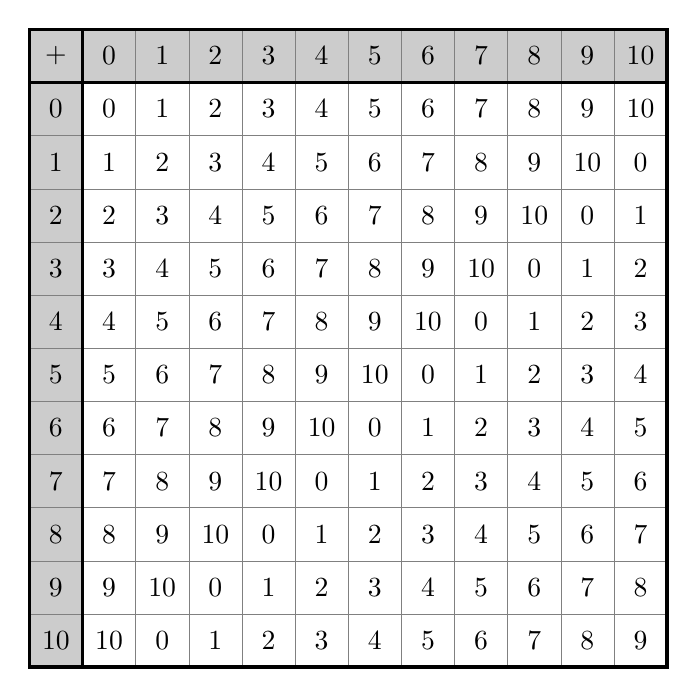
\begin{tikzpicture}[>=latex,thick,scale=0.45]
\fill[color=gray!40] (0,0) rectangle (18,-1.5);
\fill[color=gray!40] (0,0) rectangle (1.5,-18);	
\draw[step = 1.5, gray,very thin] (0,0) grid (18,-18);
\draw[very thick] (0,0) rectangle (18,-18);
\draw[very thick] (0,-1.5) -- (18,-1.5);
\draw[very thick] (1.5,0) -- (1.5,-18);
\node at (0.75,-0.75) {$+$};
\foreach \x in {0,...,10}
	\node at (2.25+\x*1.5,-0.75) {$\x$};
\foreach \y in {0,...,10}
	\node at (0.75,-2.25+\y*-1.5) {$\y$};
% Row 0
\node at ( 2.25,-2.25) {$0$};
\node at ( 3.75,-2.25) {$1$};
\node at ( 5.25,-2.25) {$2$};
\node at ( 6.75,-2.25) {$3$};
\node at ( 8.25,-2.25) {$4$};
\node at ( 9.75,-2.25) {$5$};
\node at (11.25,-2.25) {$6$};
\node at (12.75,-2.25) {$7$};
\node at (14.25,-2.25) {$8$};
\node at (15.75,-2.25) {$9$};
\node at (17.25,-2.25) {$10$};
% Row 1
\node at ( 2.25,-3.75) {$1$};
\node at ( 3.75,-3.75) {$2$};
\node at ( 5.25,-3.75) {$3$};
\node at ( 6.75,-3.75) {$4$};
\node at ( 8.25,-3.75) {$5$};
\node at ( 9.75,-3.75) {$6$};
\node at (11.25,-3.75) {$7$};
\node at (12.75,-3.75) {$8$};
\node at (14.25,-3.75) {$9$};
\node at (15.75,-3.75) {$10$};
\node at (17.25,-3.75) {$0$};
% Row 2
\node at ( 2.25,-5.25) {$2$};
\node at ( 3.75,-5.25) {$3$};
\node at ( 5.25,-5.25) {$4$};
\node at ( 6.75,-5.25) {$5$};
\node at ( 8.25,-5.25) {$6$};
\node at ( 9.75,-5.25) {$7$};
\node at (11.25,-5.25) {$8$};
\node at (12.75,-5.25) {$9$};
\node at (14.25,-5.25) {$10$};
\node at (15.75,-5.25) {$0$};
\node at (17.25,-5.25) {$1$};
% Row 3
\node at ( 2.25,-6.75) {$3$};
\node at ( 3.75,-6.75) {$4$};
\node at ( 5.25,-6.75) {$5$};
\node at ( 6.75,-6.75) {$6$};
\node at ( 8.25,-6.75) {$7$};
\node at ( 9.75,-6.75) {$8$};
\node at (11.25,-6.75) {$9$};
\node at (12.75,-6.75) {$10$};
\node at (14.25,-6.75) {$0$};
\node at (15.75,-6.75) {$1$};
\node at (17.25,-6.75) {$2$};
% Row 4
\node at ( 2.25,-8.25) {$4$};
\node at ( 3.75,-8.25) {$5$};
\node at ( 5.25,-8.25) {$6$};
\node at ( 6.75,-8.25) {$7$};
\node at ( 8.25,-8.25) {$8$};
\node at ( 9.75,-8.25) {$9$};
\node at (11.25,-8.25) {$10$};
\node at (12.75,-8.25) {$0$};
\node at (14.25,-8.25) {$1$};
\node at (15.75,-8.25) {$2$};
\node at (17.25,-8.25) {$3$};
% Row 5
\node at ( 2.25,-9.75) {$5$};
\node at ( 3.75,-9.75) {$6$};
\node at ( 5.25,-9.75) {$7$};
\node at ( 6.75,-9.75) {$8$};
\node at ( 8.25,-9.75) {$9$};
\node at ( 9.75,-9.75) {$10$};
\node at (11.25,-9.75) {$0$};
\node at (12.75,-9.75) {$1$};
\node at (14.25,-9.75) {$2$};
\node at (15.75,-9.75) {$3$};
\node at (17.25,-9.75) {$4$};
% Row 6
\node at ( 2.25,-11.25) {$6$};
\node at ( 3.75,-11.25) {$7$};
\node at ( 5.25,-11.25) {$8$};
\node at ( 6.75,-11.25) {$9$};
\node at ( 8.25,-11.25) {$10$};
\node at ( 9.75,-11.25) {$0$};
\node at (11.25,-11.25) {$1$};
\node at (12.75,-11.25) {$2$};
\node at (14.25,-11.25) {$3$};
\node at (15.75,-11.25) {$4$};
\node at (17.25,-11.25) {$5$};
% Row 7
\node at ( 2.25,-12.75) {$7$};
\node at ( 3.75,-12.75) {$8$};
\node at ( 5.25,-12.75) {$9$};
\node at ( 6.75,-12.75) {$10$};
\node at ( 8.25,-12.75) {$0$};
\node at ( 9.75,-12.75) {$1$};
\node at (11.25,-12.75) {$2$};
\node at (12.75,-12.75) {$3$};
\node at (14.25,-12.75) {$4$};
\node at (15.75,-12.75) {$5$};
\node at (17.25,-12.75) {$6$};
% Row 8
\node at ( 2.25,-14.25) {$8$};
\node at ( 3.75,-14.25) {$9$};
\node at ( 5.25,-14.25) {$10$};
\node at ( 6.75,-14.25) {$0$};
\node at ( 8.25,-14.25) {$1$};
\node at ( 9.75,-14.25) {$2$};
\node at (11.25,-14.25) {$3$};
\node at (12.75,-14.25) {$4$};
\node at (14.25,-14.25) {$5$};
\node at (15.75,-14.25) {$6$};
\node at (17.25,-14.25) {$7$};
% Row 9
\node at ( 2.25,-15.75) {$9$};
\node at ( 3.75,-15.75) {$10$};
\node at ( 5.25,-15.75) {$0$};
\node at ( 6.75,-15.75) {$1$};
\node at ( 8.25,-15.75) {$2$};
\node at ( 9.75,-15.75) {$3$};
\node at (11.25,-15.75) {$4$};
\node at (12.75,-15.75) {$5$};
\node at (14.25,-15.75) {$6$};
\node at (15.75,-15.75) {$7$};
\node at (17.25,-15.75) {$8$};
% Row 10
\node at ( 2.25,-17.25) {$10$};
\node at ( 3.75,-17.25) {$0$};
\node at ( 5.25,-17.25) {$1$};
\node at ( 6.75,-17.25) {$2$};
\node at ( 8.25,-17.25) {$3$};
\node at ( 9.75,-17.25) {$4$};
\node at (11.25,-17.25) {$5$};
\node at (12.75,-17.25) {$6$};
\node at (14.25,-17.25) {$7$};
\node at (15.75,-17.25) {$8$};
\node at (17.25,-17.25) {$9$};
\end{tikzpicture}

\end{center}


\subsection{Multiplikationstabelle
	\label{reedsolomon:subsection:mptab}}
% created by Michael Steiner
%
% Restetabelle von F_11: Multiplikation

% alternatives design
%\begin{figure}
%\begin{center}
%\begin{tabular}{|>{$}c<{$}|>{$}c<{$}>{$}c<{$}>{$}c<{$}>{$}c<{$}>{$}c<{$}>{$}c<{$}>{$}c<{$}>{$}c<{$}>{$}c<{$}>{$}c<{$}>{$}c<{$}|}
%\hline
%\cdot&0&1&2&3&4&5&6&7&8&9&10\\
%\hline
%0&0&0&0&0&0&0&0&0&0&0&0\\
%1&0&1&2&3&4&5&6&7&8&9&10\\
%2&0&2&4&6&8&10&1&3&5&7&9\\
%3&0&3&6&9&1&4&7&10&2&5&8\\
%4&0&4&8&1&5&9&2&6&10&3&7\\
%5&0&5&10&4&9&3&8&2&7&1&6\\
%6&0&6&1&7&2&8&3&9&4&10&5\\
%7&0&7&3&10&6&2&9&5&1&8&4\\
%8&0&8&5&2&10&7&4&1&9&6&3\\
%9&0&9&7&5&3&1&10&8&6&4&2\\
%10&0&10&9&8&7&6&5&4&3&2&1\\
%\hline
%\end{tabular}
%\end{center}
%\end{figure}

\begin{center}
	
	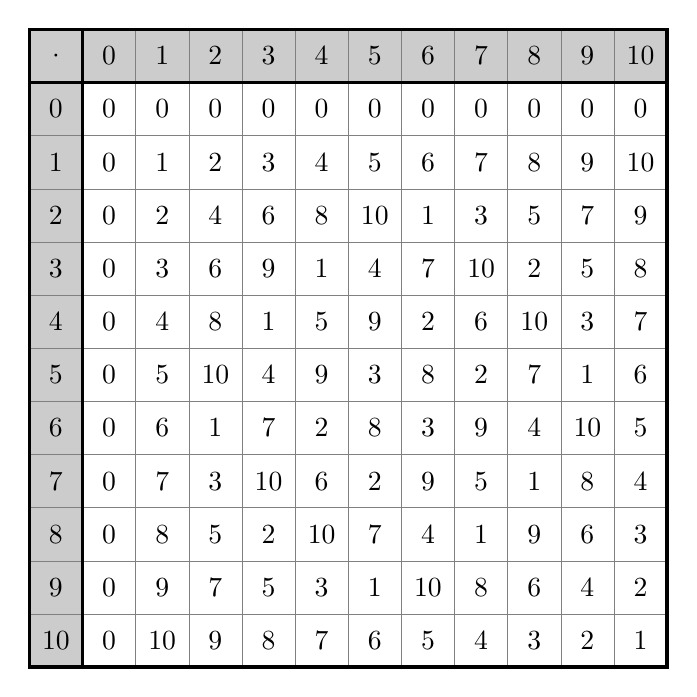
\begin{tikzpicture}[>=latex,thick,scale=0.45]
		\fill[color=gray!40] (0,0) rectangle (18,-1.5);
		\fill[color=gray!40] (0,0) rectangle (1.5,-18);	
		\draw[step = 1.5, gray,very thin] (0,0) grid (18,-18);
		\draw[very thick] (0,0) rectangle (18,-18);
		\draw[very thick] (0,-1.5) -- (18,-1.5);
		\draw[very thick] (1.5,0) -- (1.5,-18);
		\node at (0.75,-0.75) {$\cdot$};
		\foreach \x in {0,...,10}
		\node at (2.25+\x*1.5,-0.75) {$\x$};
		\foreach \y in {0,...,10}
		\node at (0.75,-2.25+\y*-1.5) {$\y$};
		% Row 0
		\node at ( 2.25,-2.25) {$0$};
		\node at ( 3.75,-2.25) {$0$};
		\node at ( 5.25,-2.25) {$0$};
		\node at ( 6.75,-2.25) {$0$};
		\node at ( 8.25,-2.25) {$0$};
		\node at ( 9.75,-2.25) {$0$};
		\node at (11.25,-2.25) {$0$};
		\node at (12.75,-2.25) {$0$};
		\node at (14.25,-2.25) {$0$};
		\node at (15.75,-2.25) {$0$};
		\node at (17.25,-2.25) {$0$};
		% Row 1
		\node at ( 2.25,-3.75) {$0$};
		\node at ( 3.75,-3.75) {$1$};
		\node at ( 5.25,-3.75) {$2$};
		\node at ( 6.75,-3.75) {$3$};
		\node at ( 8.25,-3.75) {$4$};
		\node at ( 9.75,-3.75) {$5$};
		\node at (11.25,-3.75) {$6$};
		\node at (12.75,-3.75) {$7$};
		\node at (14.25,-3.75) {$8$};
		\node at (15.75,-3.75) {$9$};
		\node at (17.25,-3.75) {$10$};
		% Row 2
		\node at ( 2.25,-5.25) {$0$};
		\node at ( 3.75,-5.25) {$2$};
		\node at ( 5.25,-5.25) {$4$};
		\node at ( 6.75,-5.25) {$6$};
		\node at ( 8.25,-5.25) {$8$};
		\node at ( 9.75,-5.25) {$10$};
		\node at (11.25,-5.25) {$1$};
		\node at (12.75,-5.25) {$3$};
		\node at (14.25,-5.25) {$5$};
		\node at (15.75,-5.25) {$7$};
		\node at (17.25,-5.25) {$9$};
		% Row 3
		\node at ( 2.25,-6.75) {$0$};
		\node at ( 3.75,-6.75) {$3$};
		\node at ( 5.25,-6.75) {$6$};
		\node at ( 6.75,-6.75) {$9$};
		\node at ( 8.25,-6.75) {$1$};
		\node at ( 9.75,-6.75) {$4$};
		\node at (11.25,-6.75) {$7$};
		\node at (12.75,-6.75) {$10$};
		\node at (14.25,-6.75) {$2$};
		\node at (15.75,-6.75) {$5$};
		\node at (17.25,-6.75) {$8$};
		% Row 4
		\node at ( 2.25,-8.25) {$0$};
		\node at ( 3.75,-8.25) {$4$};
		\node at ( 5.25,-8.25) {$8$};
		\node at ( 6.75,-8.25) {$1$};
		\node at ( 8.25,-8.25) {$5$};
		\node at ( 9.75,-8.25) {$9$};
		\node at (11.25,-8.25) {$2$};
		\node at (12.75,-8.25) {$6$};
		\node at (14.25,-8.25) {$10$};
		\node at (15.75,-8.25) {$3$};
		\node at (17.25,-8.25) {$7$};
		% Row 5
		\node at ( 2.25,-9.75) {$0$};
		\node at ( 3.75,-9.75) {$5$};
		\node at ( 5.25,-9.75) {$10$};
		\node at ( 6.75,-9.75) {$4$};
		\node at ( 8.25,-9.75) {$9$};
		\node at ( 9.75,-9.75) {$3$};
		\node at (11.25,-9.75) {$8$};
		\node at (12.75,-9.75) {$2$};
		\node at (14.25,-9.75) {$7$};
		\node at (15.75,-9.75) {$1$};
		\node at (17.25,-9.75) {$6$};
		% Row 6
		\node at ( 2.25,-11.25) {$0$};
		\node at ( 3.75,-11.25) {$6$};
		\node at ( 5.25,-11.25) {$1$};
		\node at ( 6.75,-11.25) {$7$};
		\node at ( 8.25,-11.25) {$2$};
		\node at ( 9.75,-11.25) {$8$};
		\node at (11.25,-11.25) {$3$};
		\node at (12.75,-11.25) {$9$};
		\node at (14.25,-11.25) {$4$};
		\node at (15.75,-11.25) {$10$};
		\node at (17.25,-11.25) {$5$};
		% Row 7
		\node at ( 2.25,-12.75) {$0$};
		\node at ( 3.75,-12.75) {$7$};
		\node at ( 5.25,-12.75) {$3$};
		\node at ( 6.75,-12.75) {$10$};
		\node at ( 8.25,-12.75) {$6$};
		\node at ( 9.75,-12.75) {$2$};
		\node at (11.25,-12.75) {$9$};
		\node at (12.75,-12.75) {$5$};
		\node at (14.25,-12.75) {$1$};
		\node at (15.75,-12.75) {$8$};
		\node at (17.25,-12.75) {$4$};
		% Row 8
		\node at ( 2.25,-14.25) {$0$};
		\node at ( 3.75,-14.25) {$8$};
		\node at ( 5.25,-14.25) {$5$};
		\node at ( 6.75,-14.25) {$2$};
		\node at ( 8.25,-14.25) {$10$};
		\node at ( 9.75,-14.25) {$7$};
		\node at (11.25,-14.25) {$4$};
		\node at (12.75,-14.25) {$1$};
		\node at (14.25,-14.25) {$9$};
		\node at (15.75,-14.25) {$6$};
		\node at (17.25,-14.25) {$3$};
		% Row 9
		\node at ( 2.25,-15.75) {$0$};
		\node at ( 3.75,-15.75) {$9$};
		\node at ( 5.25,-15.75) {$7$};
		\node at ( 6.75,-15.75) {$5$};
		\node at ( 8.25,-15.75) {$3$};
		\node at ( 9.75,-15.75) {$1$};
		\node at (11.25,-15.75) {$10$};
		\node at (12.75,-15.75) {$8$};
		\node at (14.25,-15.75) {$6$};
		\node at (15.75,-15.75) {$4$};
		\node at (17.25,-15.75) {$2$};
		% Row 10
		\node at ( 2.25,-17.25) {$0$};
		\node at ( 3.75,-17.25) {$10$};
		\node at ( 5.25,-17.25) {$9$};
		\node at ( 6.75,-17.25) {$8$};
		\node at ( 8.25,-17.25) {$7$};
		\node at ( 9.75,-17.25) {$6$};
		\node at (11.25,-17.25) {$5$};
		\node at (12.75,-17.25) {$4$};
		\node at (14.25,-17.25) {$3$};
		\node at (15.75,-17.25) {$2$};
		\node at (17.25,-17.25) {$1$};
	\end{tikzpicture}
	
\end{center}
%%
% anwendungen.tex -- Anwendungen des Reed-Solomon-Codes
%
% (c) 2021 Michael Steiner, Hochschule Rapperswil
%
\section{Anwendungen des Reed-Solomon-Codes
	\label{reedsolomon:section:anwendung}}

In den vorherigen Abschnitten haben wir betrachtet, wie Reed-Solomon-Codes in der Theorie funktionieren. 
In diesem Abschnitt werden wir einige Anwendungen vorstellen, bei denen ein Reed-Solomon-Code zum Einsatz kommt.

All diese Anwendungen teilen das gleiche Problem: Die Daten können nur durch einen höchstwahrscheinlich fehlerbehafteten Kanal empfangen werden. Es gibt keine andere Methode, an diese Daten zu kommen, als über diesen Kanal.

\rhead{Anwendungen}
In der Netzwerktechnik zum Beispiel ist es üblich, dass bei Paketverlusten oder beschädigt empfangenen Datenpaketen diese einfach noch einmal innert weniger Millisekunden angefordert werden können.
\index{Paketverluste}%
In der Raumfahrt ist dies nicht möglich, da aufgrund der beschränkten Speichermöglichkeit die gesammelten Daten so rasch wie möglich zur Erde gesendet werden. 
\index{Raumfahrt}%
Diese Daten wiederum brauchen aufgrund der grossen Distanz Stunden, bis sie beim Empfänger ankommen.
Fehlerhafte Daten können also auf Grund der Zeitverzögerung nicht mehr angefordert werden. 

Bei CDs oder DVDs gibt es zwar kein zeitliches Problem, jedoch erschweren Kratzer, Verschmutzungen oder Produktionsfehler das Lesen einer solchen Disk.
\index{CD}%
\index{Compact-Disc}%
\index{DVD}%
\index{Digital Video Disk}%
Da vor allem Produktionsfehler und Kratzer irreversibel sind und die Disk nicht nach jedem Kratzer ersetzt werden, wird die korrekte Ausgabe der gespeicherten Information durch die Fehlerkorrektur sichergestellt. 

Einen ähnlichen Ansatz verfolgen QR-Codes, wobei die Information auch dann noch gelesen werden kann, wenn der Code nicht mehr vollständig vorhanden ist. 
\index{QR-Code}%

%Wie man sieht, eignen sich Reed-Solomon-Codes vor allem für Anwendungen, bei der die Informationen nicht auf einen Anderen Weg beschafft werden kann. 
%
%
%, bei denen die Wahrscheinlichkeit hoch ist, dass während der Übertragung 
%
%Es ist deshalb umso wichtiger die Daten codiert zu lesen um so gleich die Lesefehler zu korrigieren.
%
% da aufgrund der grossen Distanz Stunden vergehen können bis gesendete Daten auf der Erde empfangen werden kann. 
%

Obwohl all diese Codes nach dem gleichen Prinzip arbeiten, gibt es starke Unterschiede in deren Funktionsweise. 
Dies kommt vor allem daher, dass die Codes nur Ressourcen zur Verfügung haben, die von der Hardware bereitgestellt werden, auf denen die Codes implementiert wurden.
Diese Codes bedienen sich daher verschiedener Tricks und Optimierungen, um möglichst effizient zu arbeiten.

Um die Fähigkeit eines verwendeten Reed-Solomon-Codes zu beschreiben, verwendet man die Notation ($n$,$k$), wobei $n$ die Grösse des Nachrichtenblocks angibt und $k$ die Anzahl der Stellen, die für Nutzdaten gebraucht werden können.

%Dies kommt vor allem daher, da diese Codes an ihre Hardware gebunden sind, auf denen sie implementiert worden sind.
%Deshalb wurden diese Codes stark optimiert damit sie möglichst Effizient arbeiten können. 
%
%Um diese Hardware möglichst effizient zu nutzen wurden gewisse mathematische tricks angewendet um den Code möglichst effizient zu nutzen. 
%
% um mit maximaler Effizienz zu arbeiten. 
%Es überrascht daher nicht, dass vor allem ältere Codes im binären Körper $\mathbb{F}_{2}$ arbeiten.
%
% um den Code mit maximaler Effizienz zu nutzen. 
%
%Alle diese Anwendungen verfügen über eigene spezifizierten Eigenschaften.
%
%, wobei bei allen dieser Anwendungen jeweils eine unterschiedliche Version des Codes implementiert wurden.
%
%Dies kommt vor allem daher, da diese Codes immer an ihre dementsprechende Hardware gebunden sind, auf denen sie implementiert wurden um den Code mit maximaler Effizienz zu nutzen. 
%
% eigene Version des Codes implementiert haben. 
%
%Bei einer Technischen Umsetzung eines solchen Codes werden wir auf eine reihe neuer Probleme stossen wie Ressourceneffizienz, Laufzeitoptimierung, usw.
%
%Hinzu kommt, dass für verschiedene Anwendungen verschiedene Versionen des Reed-Solomon-Codes zur Anwendung kommen.
%
%Nachfolgend werden wir ein paar dieser Anwendungen Vorstellen, da sich herausstellt, dass Reed-Solomon-Code sehr 
%
%Als letzte Frage stellt sich jetzt nur noch, wo diese Codes eingesetzt werden. 
%
%Bisher haben wir 
%
%In den letzten abschnitten haben wir uns ausführlich die Funktionsweise des Reed-Solomon-Codes angeschaut. In diesem Abschnitt möchten wir dem Leser ein paar bekannte beispiele vorstellen, in denen Reed-Solomon-Codes zum einsatz kommen. Es sei jedoch angemerkt, dass diese Anwendungen in der Umsetzung oft ein wenig anderst funktionieren als hier vorgestellt. Dies wurde vor allem wegen technischen optimierungen realisiert. (technische tricks und finessen), von der logik jedoch sehr stark an unserem Beispiel orientieren

\begin{figure}
	\centering
	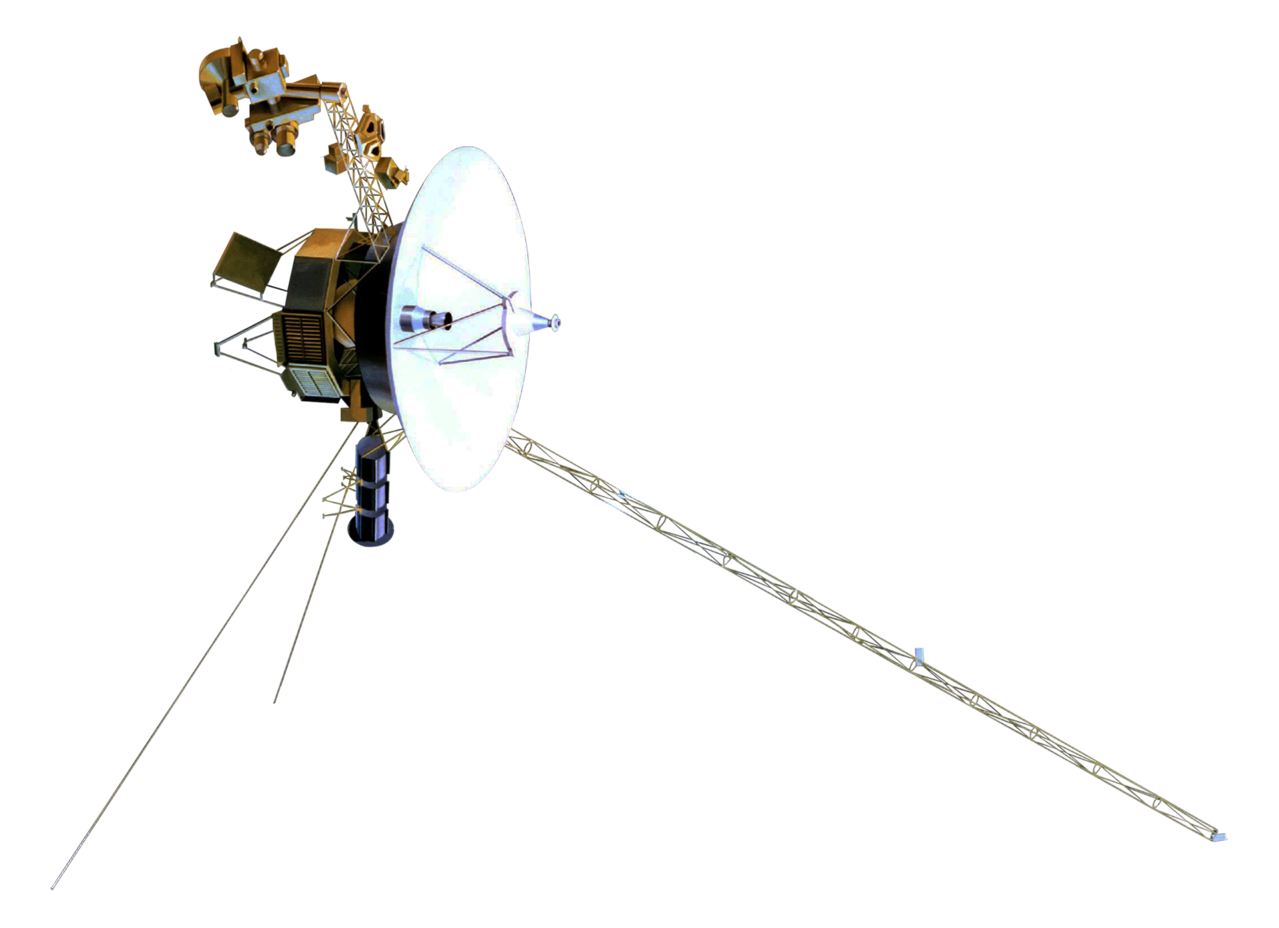
\includegraphics[width=0.5\textwidth]{papers/reedsolomon/images/Voyager_Sonde}
	\caption{Mit einer Entfernung von über 22.8 Milliarden Kilometer ist die Voyager 1 Raumsonde das am weitesten entfernte, von Menschen erschaffene Objekt. Obwohl ihre Schwestersonde Voyager 2 zuerst ins All gestartet wurde, befindet sie sich ``nur'' 19 Milliarden Kilometer weit weg von der Erde. Aufgrund abnehmender Batterieleistung werden die beiden Sonden ihre wissenschaftlichen Aktivitäten etwa 2025 einstellen, bleiben aber bis in die 2030er Jahre mit uns in Kontakt.}
\index{Voyager 1 und 2}%
	\label{fig:voyager}
\end{figure}

\subsection{Raumfahrt}
Obwohl Reed-Solomon-Codes bereits in den 1960er Jahren entwickelt wurden, fanden sie erstmals Anwendung in der Voyager Raumsonde der NASA. Die Daten der zwei im Jahre 1977 gestarteten Sonden (siehe Abbildung \ref{fig:voyager}) werden mit einem ($255$,$233$)-Code
\index{Voyager Raumsonde}%
\index{NASA}%
codiert. 
Der Nachrichtenblock hat somit eine Länge von $255$ Zahlen, wovon $233$ als Nutzlast zur Verfügung stehen.
Damit ist es möglich, bis zu $11$ Fehler im Nachrichtenblock zu korrigieren. 
Der codierte Nachrichtenblock wird in kleinere Blöcke aufgeteilt, mit einem Faltungscode erneut codiert und anschliessend gesendet.
Ein Faltungscode ist wie ein Reed-Solomon-Code in der Lage, Fehler zu korrigieren, 
codiert seine Information aber auf eine andere Weise. Aus jedem unterteilten Block wird vor dem Versenden ein Paritätsbit erzeugt und dem Block angehängt. Anhand dieses Paritätsbits überprüft der Empfänger, ob bei der Übertragung der Block beschädigt wurde. Ist dies der Fall, wird der Block bei der Decodierung nicht beachtet. Diese so entstandenen ``Lücken'' im Datenstrom werden wiederum vom Reed-Solomon-Code korrigiert. Dieses Zusammenspiel beider Codes garantiert so eine hohe Robustheit gegenüber Übertragungsfehler. 

\begin{figure}
	\centering
	\subfigure[]{
	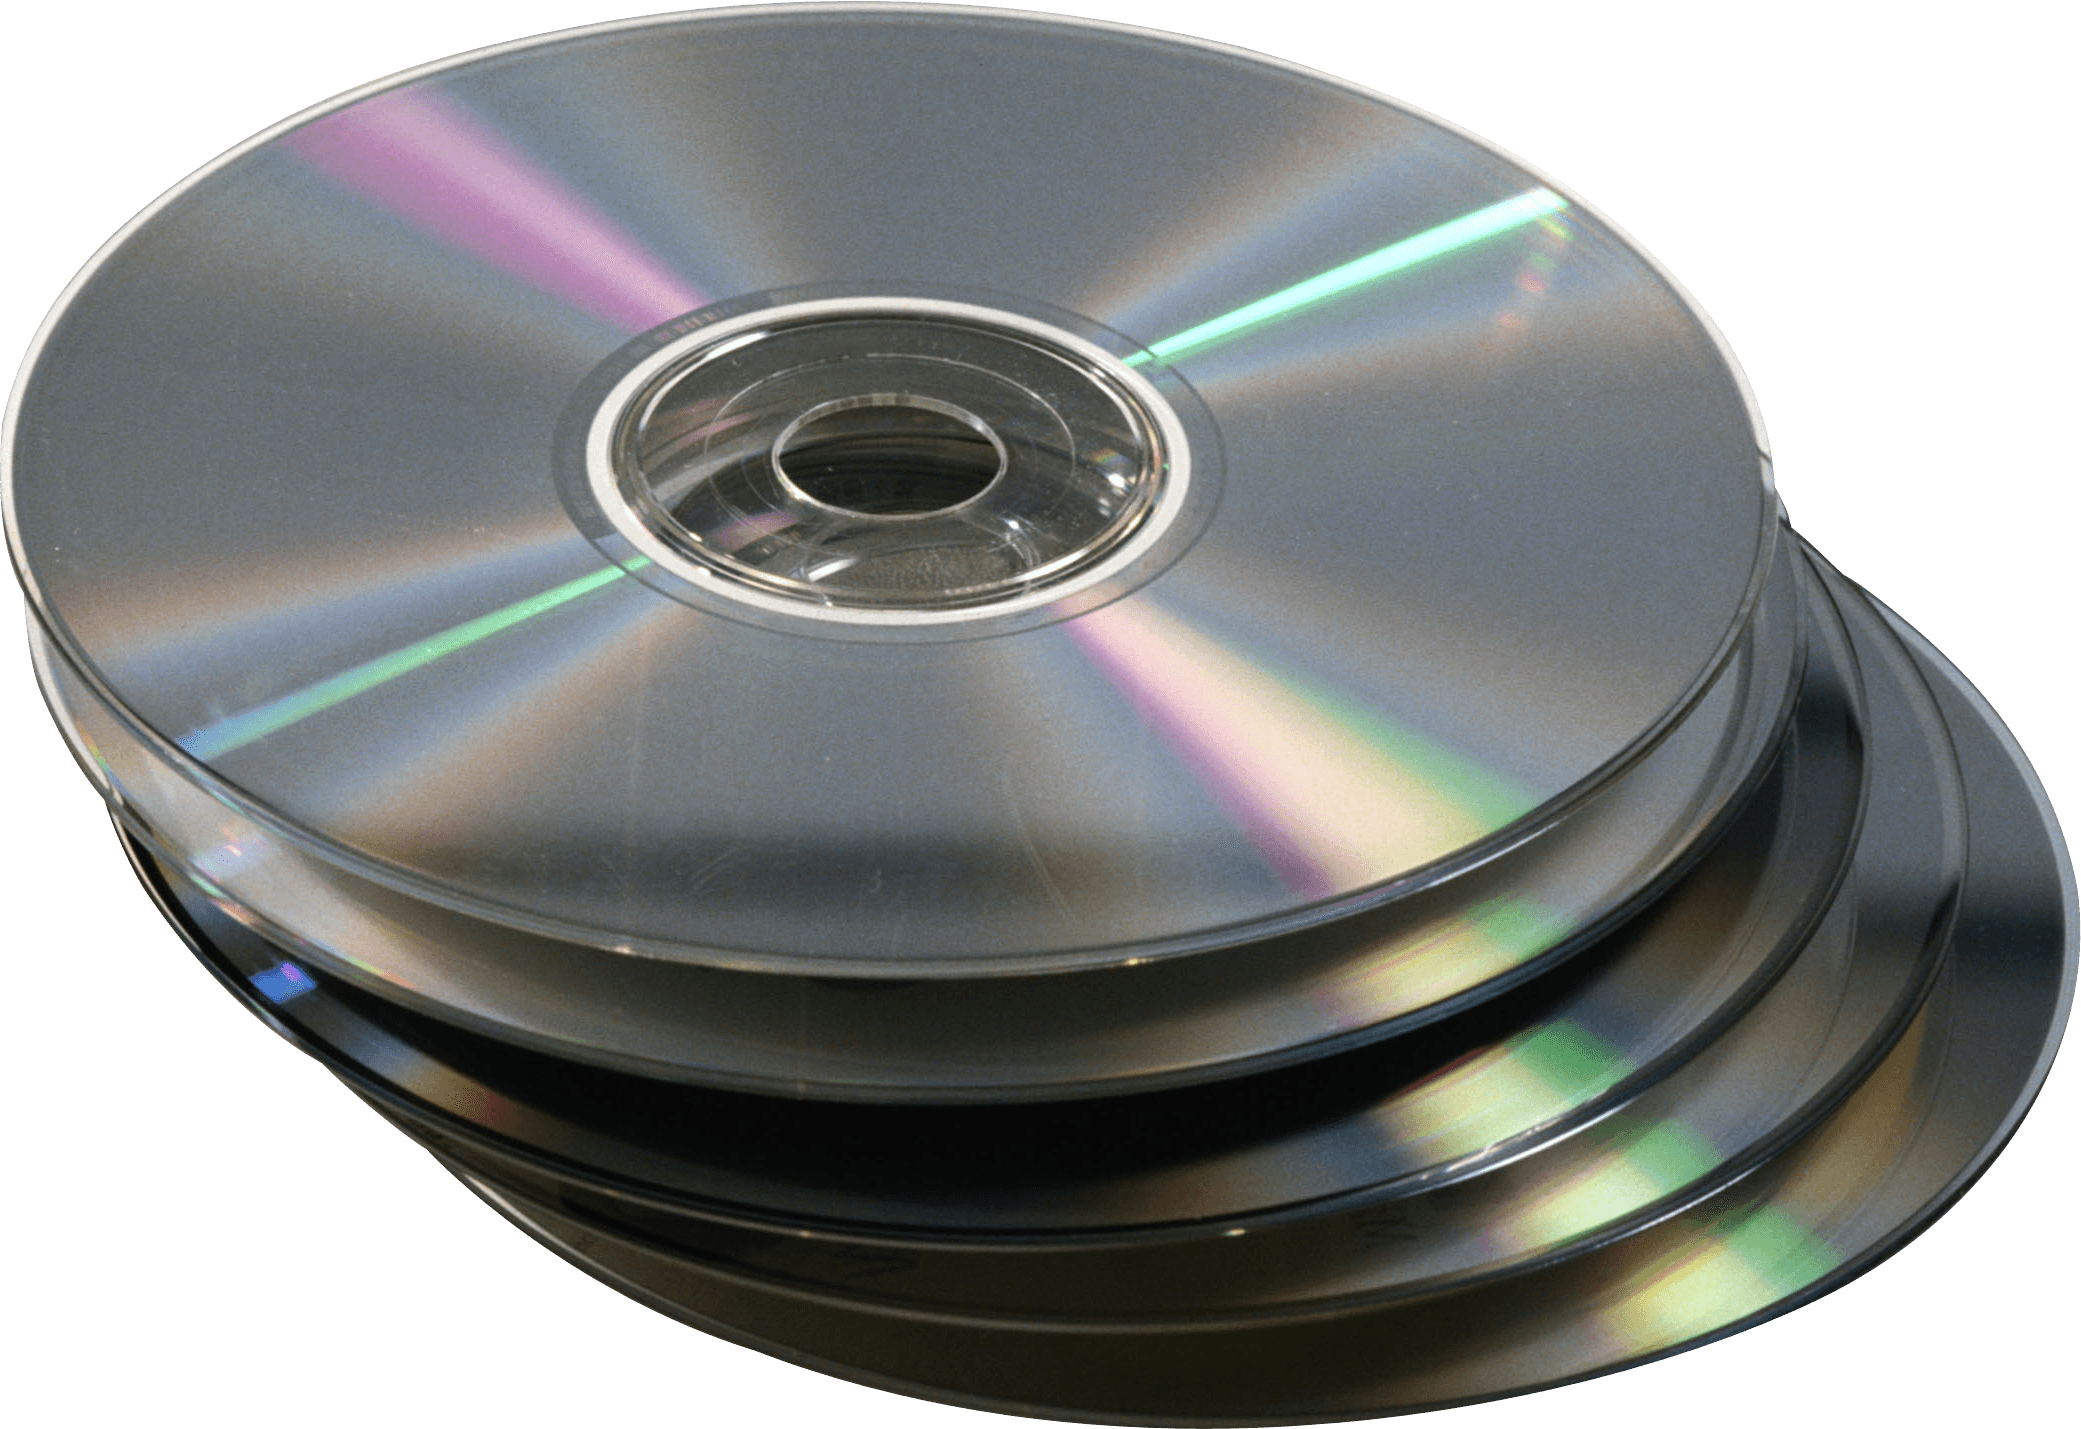
\includegraphics[width=0.45\textwidth]{papers/reedsolomon/images/Compact_Disc}
	}
	\subfigure[]{
		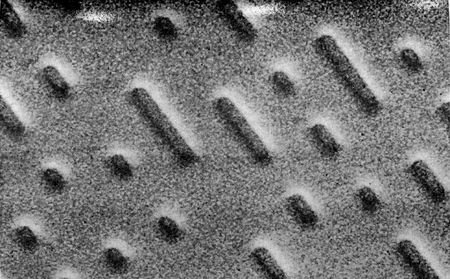
\includegraphics[width=0.45\textwidth]{papers/reedsolomon/images/Compact_Disc_zoomed_in}
	}
	\caption{CDs kamen 1982 auf den Markt. Sie funktionieren durch das Einpressen oder Einbrennen von Punkten und Strichen, die die Daten repräsentieren. Gelesen werden diese wiederum durch die Reflektion eines Lasers an diesen Punkten und Strichen.}
	\label{fig:cd}
\end{figure}
% 
% Funktioniert aber nach einem ganz anderen Prinzip. 
%
%Durch diese doppelte Codierung wird eine äusserst hohe Übertragungssicherheit garantiert.
%
%Dabei steht die Zahl 255 für grösse des Nachrichtenblocks, der die Anzahl 233
%
%
% \textcolor{red}{benötigt das weitere Erklärungen, wie z.b. 255: grösse Nachrichtenblock, 233: anzahl der nutzbaren daten ?} zusammen mit einem konventionellen Faltungscode übertragen. Eine von der Sonde gesendete Nachricht hat eine Blockgrösse von 255 Zeichen, wovon 233 für die Nutzdaten gebraucht werden können. Dieser Code ist somit in der Lage 11 Fehler in einem Nachrichtenblock zu korrigieren. 
%
% Die zwei im Jahre 1977 gestarteten Sonden senden Daten mit der Hilfe eines RS(255,233)-Code für die digitalen Bilder sowie einem konventionellen Faltungscode.
%
%
%mit der Erde mit einem RS(255,233)-Code für die digitalen Bilder sowie einem konventionellen Faltungscode. 


\subsection{CD/DVD}
Compact Discs verwenden sogar zwei ineinander verschachtelte Reed-Solomon-Codes, einen (32,28)-Code und einen (28,24)-Code.
Beide Codes sind in der Lage, Fehler aus dem jeweils anderen gelesenen Block zu korrigieren. Dieses spezielle Zusammenspielen dieser beiden Codes wird auch Cross-interleaved Reed-Solomon-Code (CIRC) genannt.
\index{CIRC}%
\index{Cross-interleaved Reed-Solomon code}%
Diese Vorgehensweise erzielt eine hohe Robustheit gegenüber Produktionsfehlern oder Verschmutzung auf der Disc. Bei CDs sind diese in der Lage, bis zu 4000 fehlerhafte Bits am Stück (ca. $2.5$mm) zu erkennen und zu korrigieren. 

Die Digital Video Disc funktioniert nach dem selben Konzept mit grösseren Codeblöcken. Die DVD verwendet einen (208,192)-Code und einen (182,172)-Code.

%Beide lesen 
% wobei beide Codes auch Fehler aus dem jeweiligen anderen Block korrigieren

\begin{figure}
	\centering
	\subfigure[]{
	
\includegraphics[width=0.4\textwidth]{papers/reedsolomon/images/qrcode_h}
	}
	\subfigure[]{
	
\includegraphics[width=0.4\textwidth]{papers/reedsolomon/images/qrcode_l}
	}
%	\subfigure[]{
%	
\includegraphics[width=0.4\textwidth]{papers/reedsolomon/images/designer_qrcode_ohnelogo}
%	}
%	\subfigure[]{
%	
\includegraphics[width=0.4\textwidth]{papers/reedsolomon/images/designer_qrcode}
%	}
	\caption{Anhand der Grösse würde man darauf schliessen, dass bei (a) mehr Informationen codiert sind als bei (b). Tatsächlich aber beinhalten beide Codes die gleiche Information. Das liegt daran, dass die Fehlerkorrekturfähigkeit von QR-Codes sich in insgesamt vier Levels aufteilen lassen. Das höchste Fehlerkorrektur-Level, das bei (a) angewendet wurde, ist in der Lage, bis zu 30\% der Daten wiederherzustellen. Das kleinste Level schafft etwa 7\%, das in (b) veranschaulicht wird. Da die Grösse also nichts über die Menge an Daten aussagt, könnte es sich bei (a) auch um einen Code mit viel Nutzdaten und kleinem Fehlerkorrektur-Level handeln. Der Unterschied ist von Auge nicht sichtbar.}
	\label{fig:qr}
\end{figure}

\begin{figure}
	\centering
%	\subfigure[]{
%		
\includegraphics[width=0.4\textwidth]{papers/reedsolomon/images/qrcode_h}
%	}
%	\subfigure[]{
%		
\includegraphics[width=0.4\textwidth]{papers/reedsolomon/images/qrcode_l}
%	}
	\subfigure[]{
		
\includegraphics[width=0.4\textwidth]{papers/reedsolomon/images/designer_qrcode_ohnelogo}
	}
	\subfigure[]{
		
\includegraphics[width=0.4\textwidth]{papers/reedsolomon/images/designer_qrcode}
	}
	\caption{Während (a) noch einen unveränderten QR-Code repräsentiert, handelt es sich bei (b) nun um einen Designer-QR-Code. Beide Codes verfügen über einen mittleren Fehlerkorrektur-Level von theoretisch 15\%. Da bei (b) jetzt ein Teil des Codes durch ein Logo verdeckt wird, schränkt sich die Fehlerkorrekturfähigkeit je nach Grösse des verdeckten Teils mehr oder weniger stark ein. Unser Designer-Code in (b) ist nur noch in der Lage, etwa 9\% des Codes zu rekonstruieren.}
	\label{fig:designqr}
\end{figure}

\subsection{QR-Codes}
\index{QR-Code}%
Quick Response Codes oder auch QR-Codes funktionieren nach einem sehr ähnlichen Prinzip wie in unserem Beispiel die Abschnitte \ref{reedsolomon:section:codebsp} - \ref{reedsolomon:section:rekonstruktion}, nur der QR-Code in einem $\mathbb{F}_{256}$ Körper arbeitet.
Die physische Grösse eines Codes ist stark abhängig von der Menge an codierten Daten sowie dem verwendeten Fehlerkorrektur-Level.
Es ist so auf den ersten Blick nicht ersichtlich, wie viel Nutzinformationen ein QR-Code enthält.
Die QR-Codes in Abbildung \ref{fig:qr} zeigen jeweils die gleiche Information mit unterschiedlichem Fehlerkorrektur-Level.
Codes mit einem höheren Korrektur-Level können auch für Designer-Codes zweckentfremdet werden.
\index{Designed-QR-Code}%
Dabei wird z.~B.~das Firmenlogo oder ein Schriftzug über den QR-Code gelegt, ohne dass die Funktion des Codes beeinträchtigt wird. Ein Beispiel dazu ist in Abbildung \ref{fig:designqr} zu finden. 

% 

%So kann auf den ersten Blick nicht 
%
%
% funktionieren nach einem sehr ähnlichen Prinzip wie in unserem Beispiel, nur dass QR-Codes in einem $\mathbb{F}_{256}$ Körper arbeiten. Je nach grösse der Codierung ist der QR-Code im Endeffekt robuster gegen Beschädigungen. Bei Low Level Codes können 7\% der Daten Wiederhergestellt werden, beim High Level Code sind das sogar 30\%. 

		-> geplant

\nocite{reedsolomon:weitz}
\nocite{reedsolomon:informationkommunikation}
%\nocite{reedsolomon:mendezmueller}

\printbibliography[heading=subbibliography]
\end{refsection}
